\documentclass{beamer}
\usetheme{metropolis}           % Use metropolis theme
\usepackage{appendixnumberbeamer}
\usepackage{epigraph}
\usepackage{color}
\usepackage{amsopn}
\usepackage{tabto}

%%% Bibliography
\usepackage[backend=bibtex, style=authoryear]{biblatex}
\AtBeginBibliography{\tiny}
\bibliography{../bibliography.bib}

\setbeamercolor{background canvas}{bg=white}
\setbeamercolor{title}{fg=gray!60}
\setbeamercolor{subtitle}{fg=gray!20}
\setbeamercolor{author}{fg=gray!60}
\setbeamercolor{institute}{fg=gray!20}

\newcommand{\todo}{\alert{TODO}}
\newcommand{\itemBullet}{\scriptsize$\blacksquare$}
\setbeamertemplate{itemize item}{\itemBullet}
\setbeamertemplate{itemize subitem}{\itemBullet}
\setbeamertemplate{itemize subsubitem}{\itemBullet}
\newcommand{\E}{\mathop{\mathbb{E}}}
\DeclareMathOperator*{\argmax}{arg\,max}
\newcommand{\epiParSpace}{\vskip 1.5ex}
\newcommand{\p}{\mathbf{p}}

\title{AlphaZero}
\subtitle{Mastering Chess and Shogi \\
by Self-Play \\ 
with a General Reinforcement Learning Algorithm }
\date{}                         % no dates
\author{Karel Ha \\ article by Google DeepMind}
\institute{AI Seminar, 19\textsuperscript{th} December 2017}

\begin{document}
  {
    \usebackgroundtemplate{
      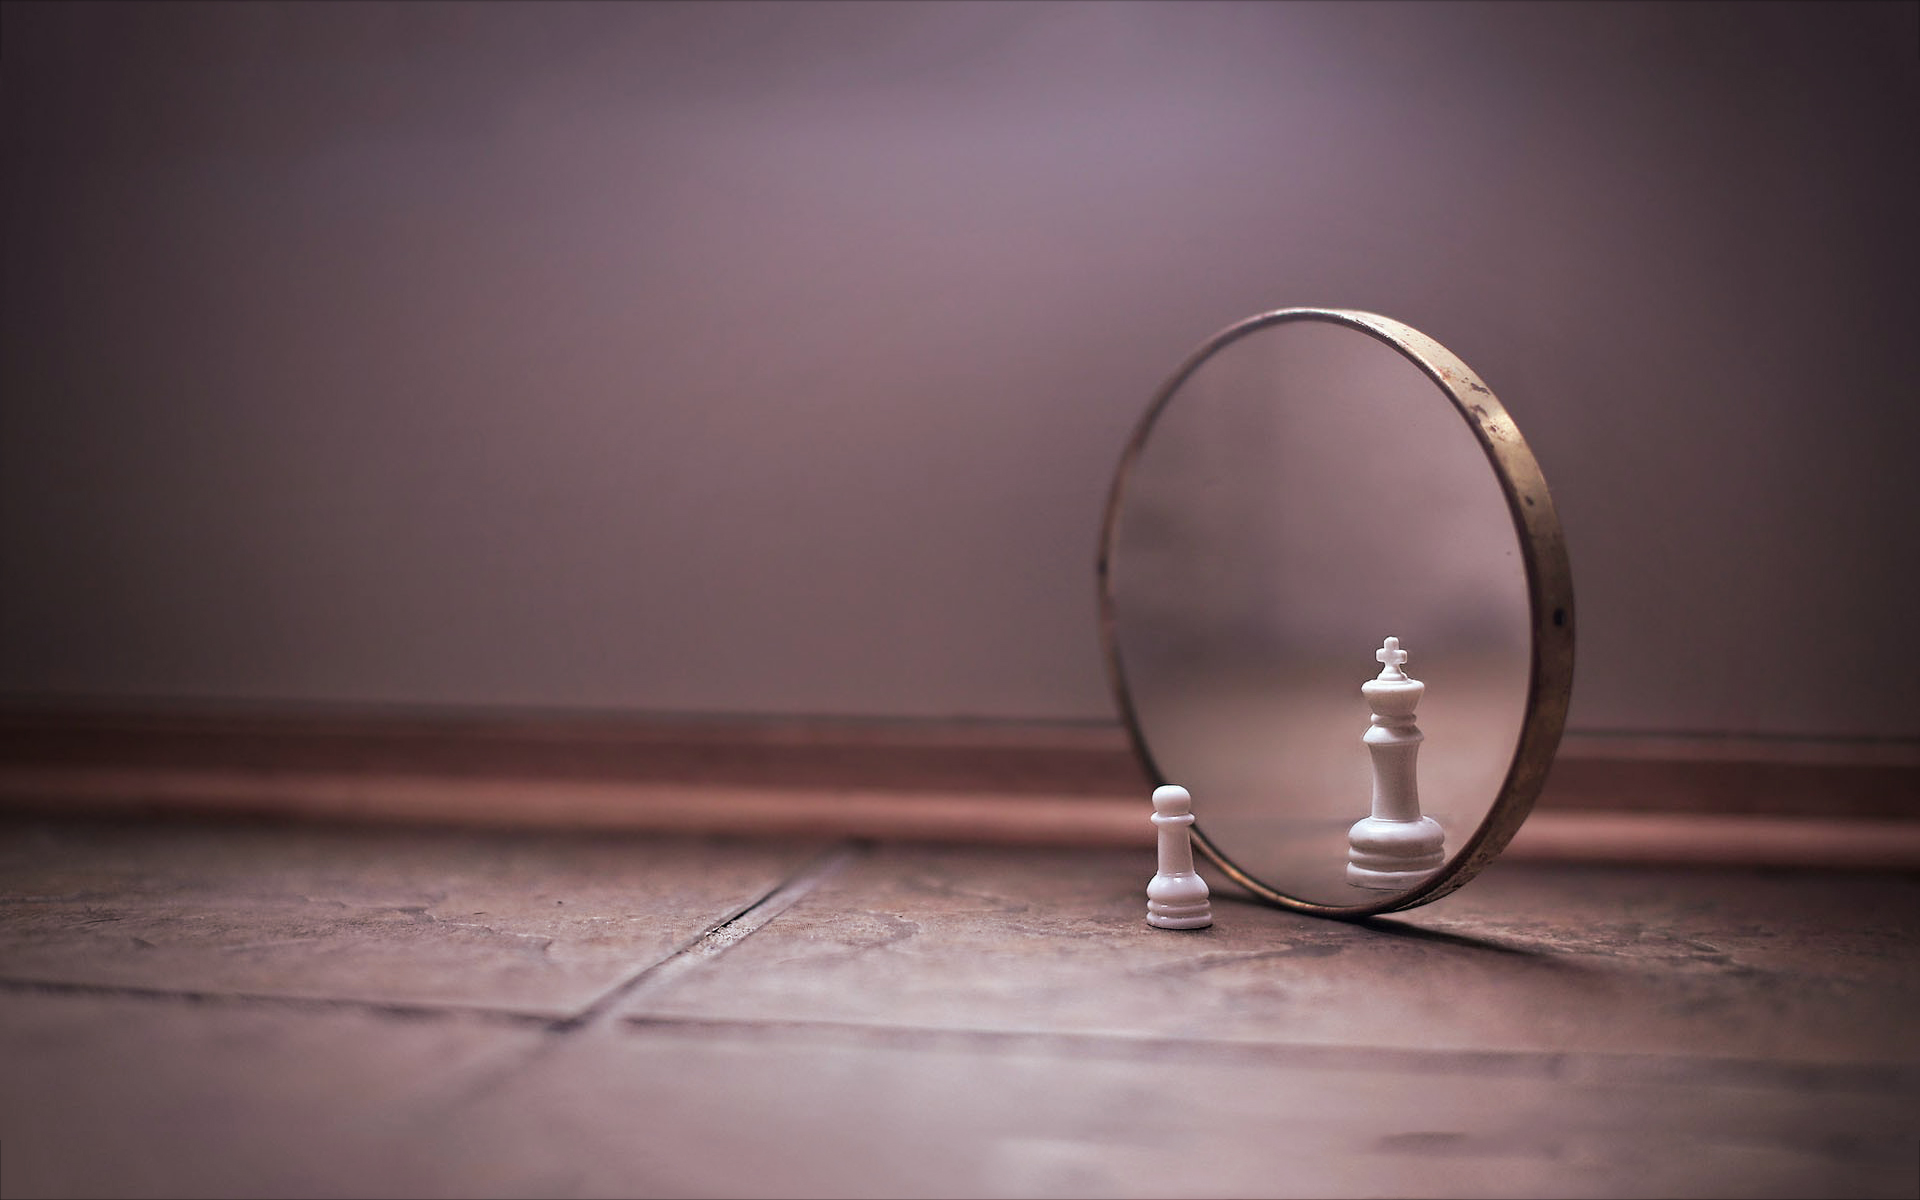
\includegraphics[height=\paperheight]{../img/cover_background.jpg}
    }
    \maketitle
  }

%%%%%%%%%%%%%%%%%%%%%%%%%%%%%%%%%%%%%%%%%%%%%%%%%%%%%%%%%%%%%%%%%%%%%%%%%%%%%%%%

  \section{The Alpha* Timeline}
  {
    \setbeamertemplate{frame footer}{\url{https://en.wikipedia.org/wiki/Fan_Hui}}
    \begin{frame}{Fan Hui}
      \begin{center}
        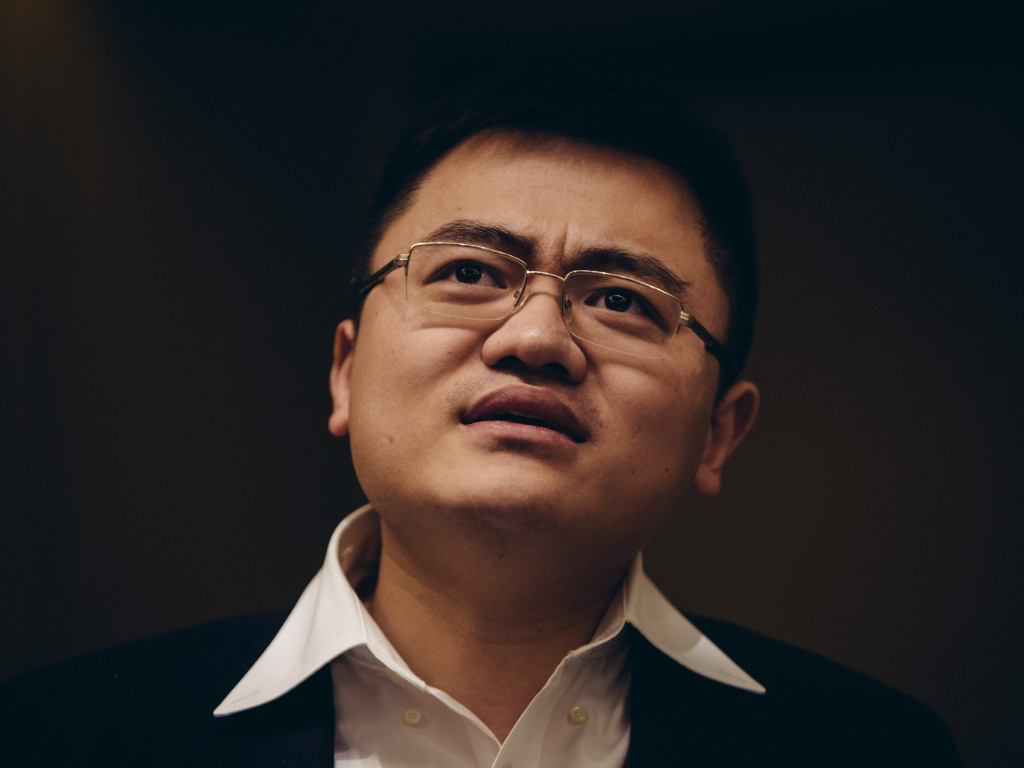
\includegraphics[width=.55\textwidth]{../img/Fan_Hui_profile.jpg}
      \end{center}
      \pause
      \vskip -1.6em
      \begin{itemize}[<+- | alert@+>]
        \item professional 2 dan
        \item European Go Champion in 2013, 2014 and 2015
        \item European Professional Go Champion in 2016 
      \end{itemize}
    \end{frame}
  }

  \begin{frame}{AlphaGo vs. Fan Hui}
    \pause
    \begin{center}
      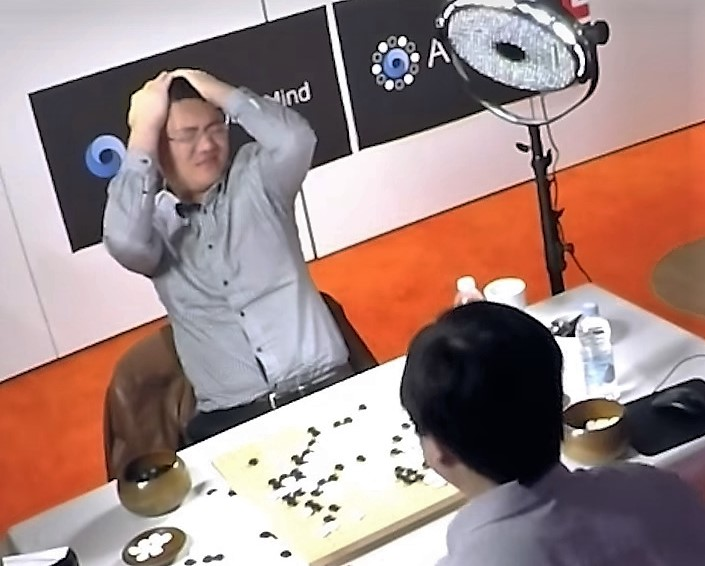
\includegraphics[width=.55\textwidth]{../img/Fan_Hui_loses.jpg}
    \end{center}
    \textbf{AlphaGo won 5:0} in a~formal match on~October 2015.
    \pause

    \vskip -1em
    \epigraph{
      \tiny
      [AlphaGo] is very strong and stable, it seems like a~wall.
      ...
      I know AlphaGo is a~computer, but if no one told me, maybe I would think the player was a~little strange, but a~very strong player, a~real person.
    }{Fan Hui}
  \end{frame}

  {
    \setbeamertemplate{frame footer}{\url{https://en.wikipedia.org/wiki/Lee_Sedol}}
    \begin{frame}{Lee Sedol ``The Strong Stone''}
      \begin{center}
        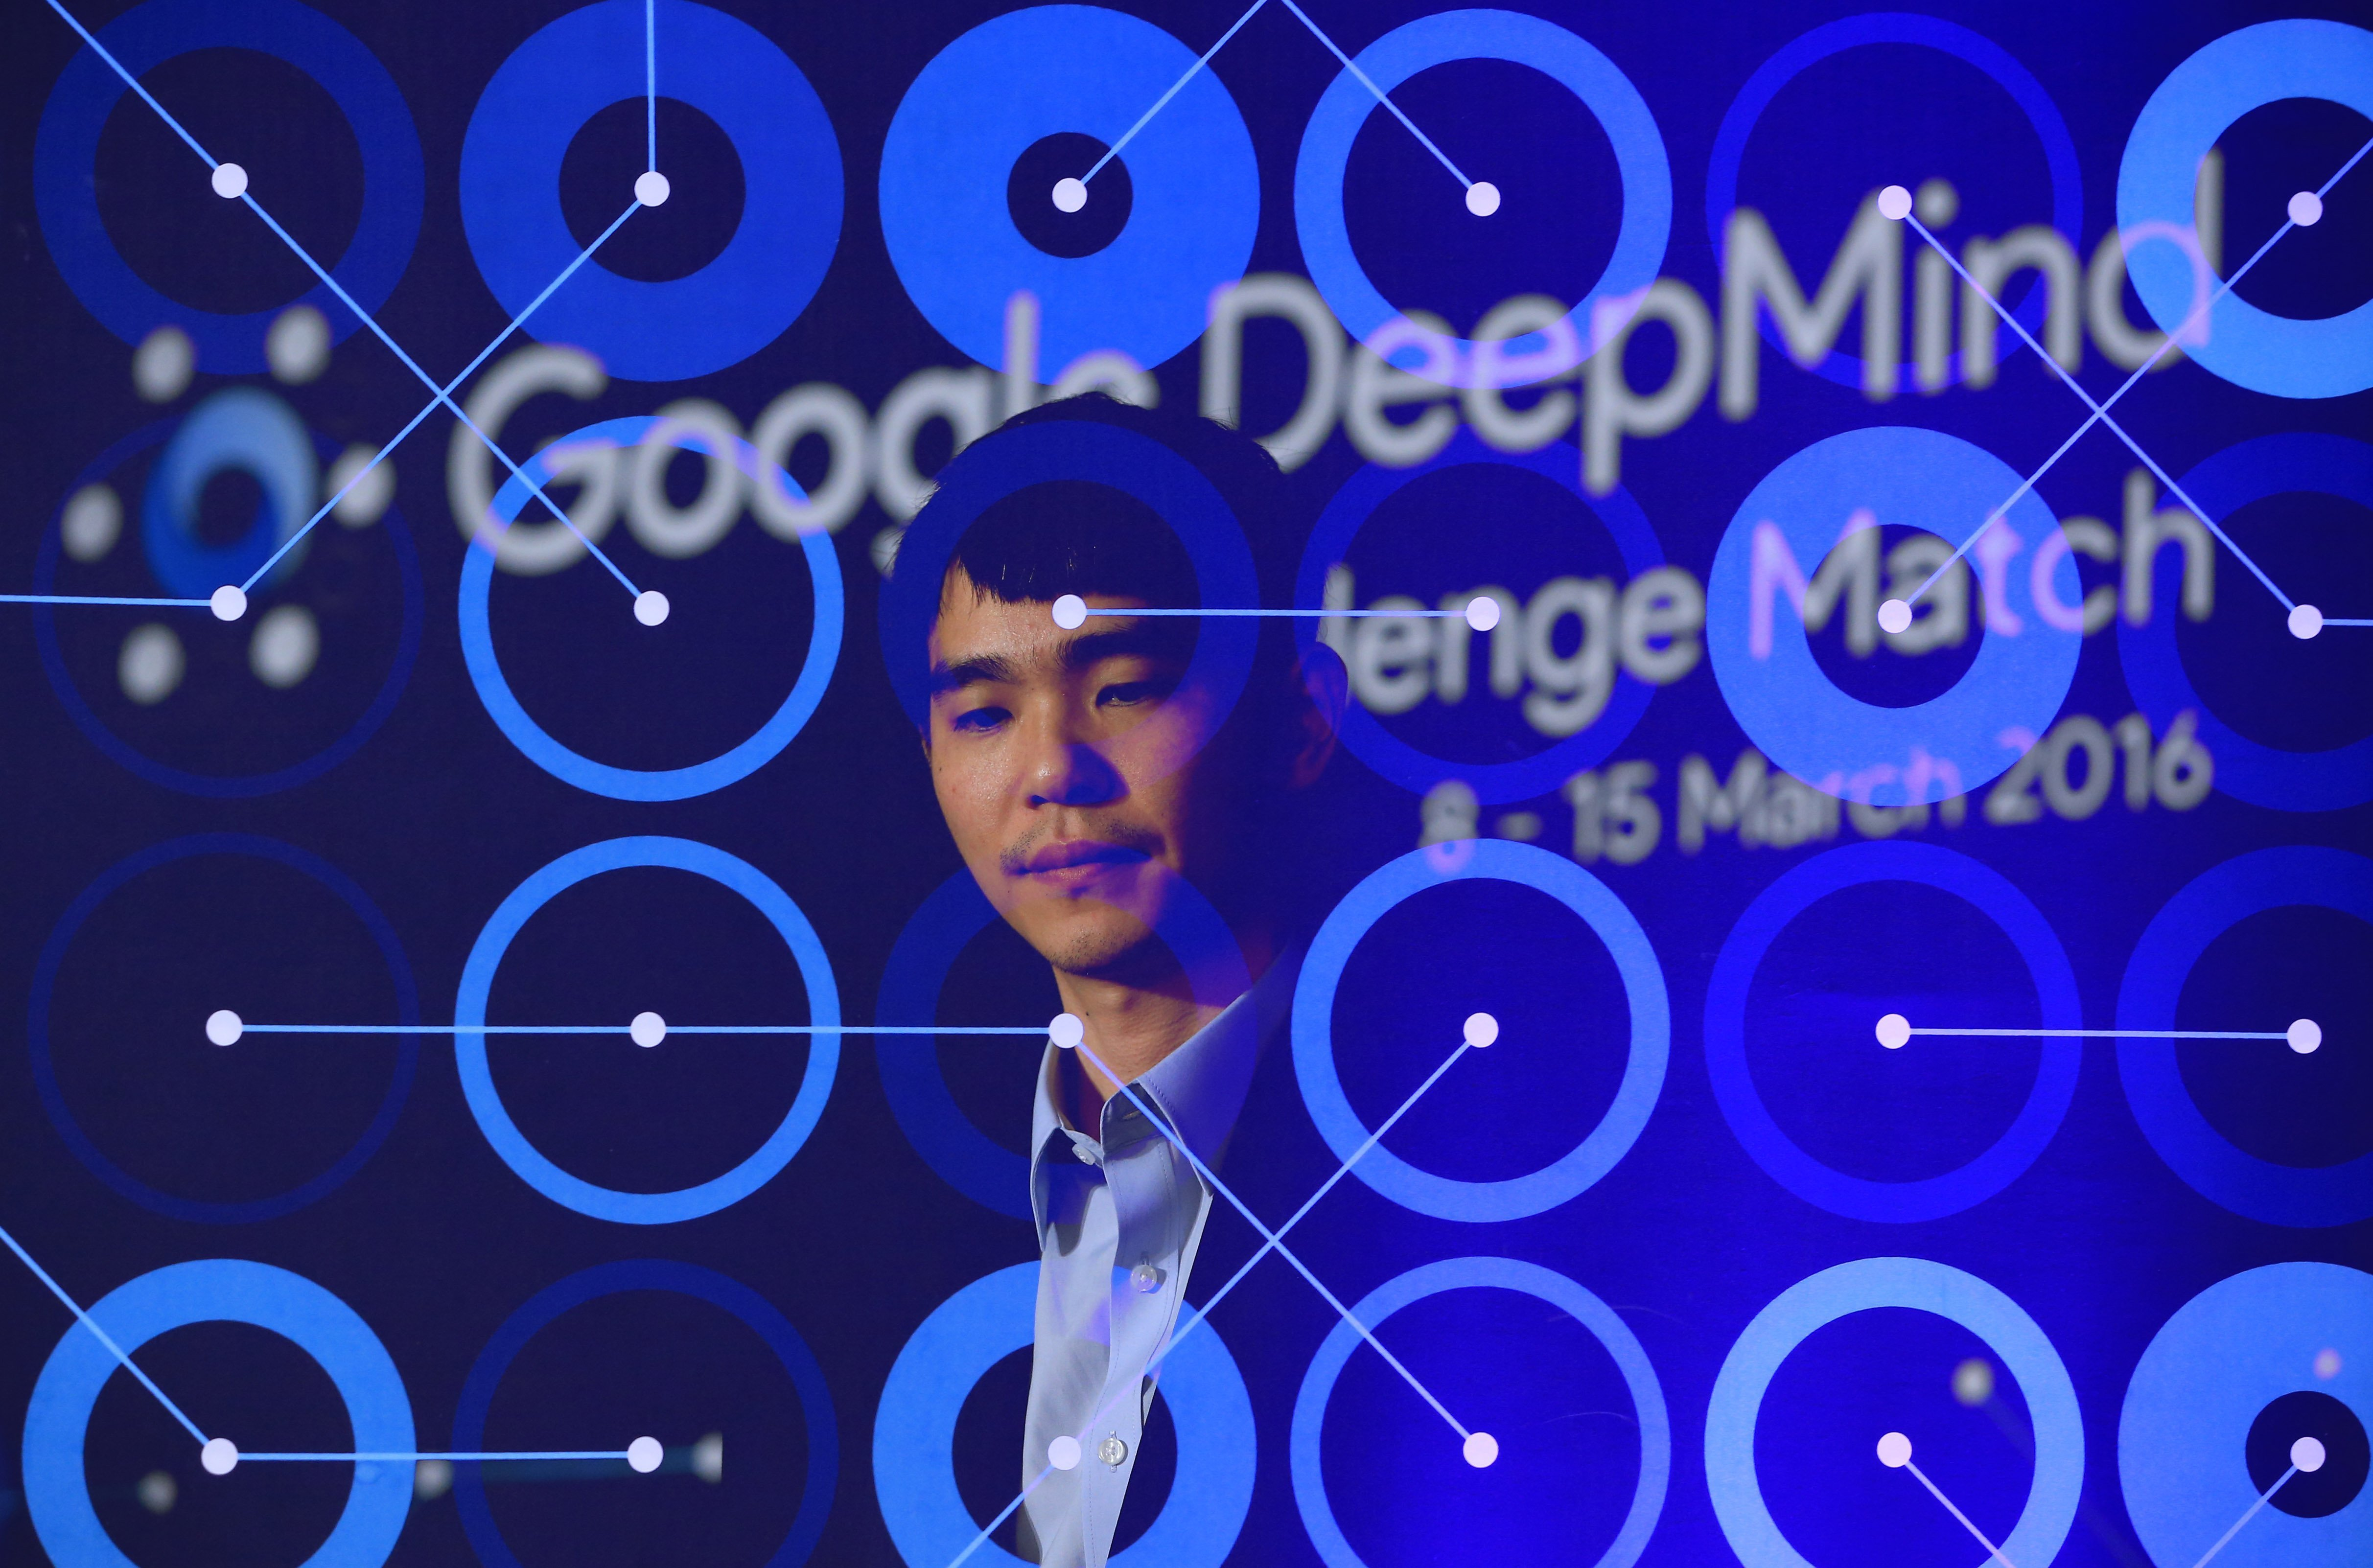
\includegraphics[width=.55\textwidth]{../img/Lee_Sedol_profile_2.jpg}
      \end{center}
      \pause
      \vskip -1.6em
      \begin{itemize}[<+- | alert@+>]
        \item professional 9 dan 
        \item the $2^{nd}$ in international titles
        \item the $5^{th}$ youngest to become a~professional Go player in~South Korean history
        \item Lee Sedol would win 97 out of~100 games against Fan Hui.
        \item ``Roger Federer'' of~Go
      \end{itemize}
    \end{frame}
  }

  {
    \usebackgroundtemplate{
      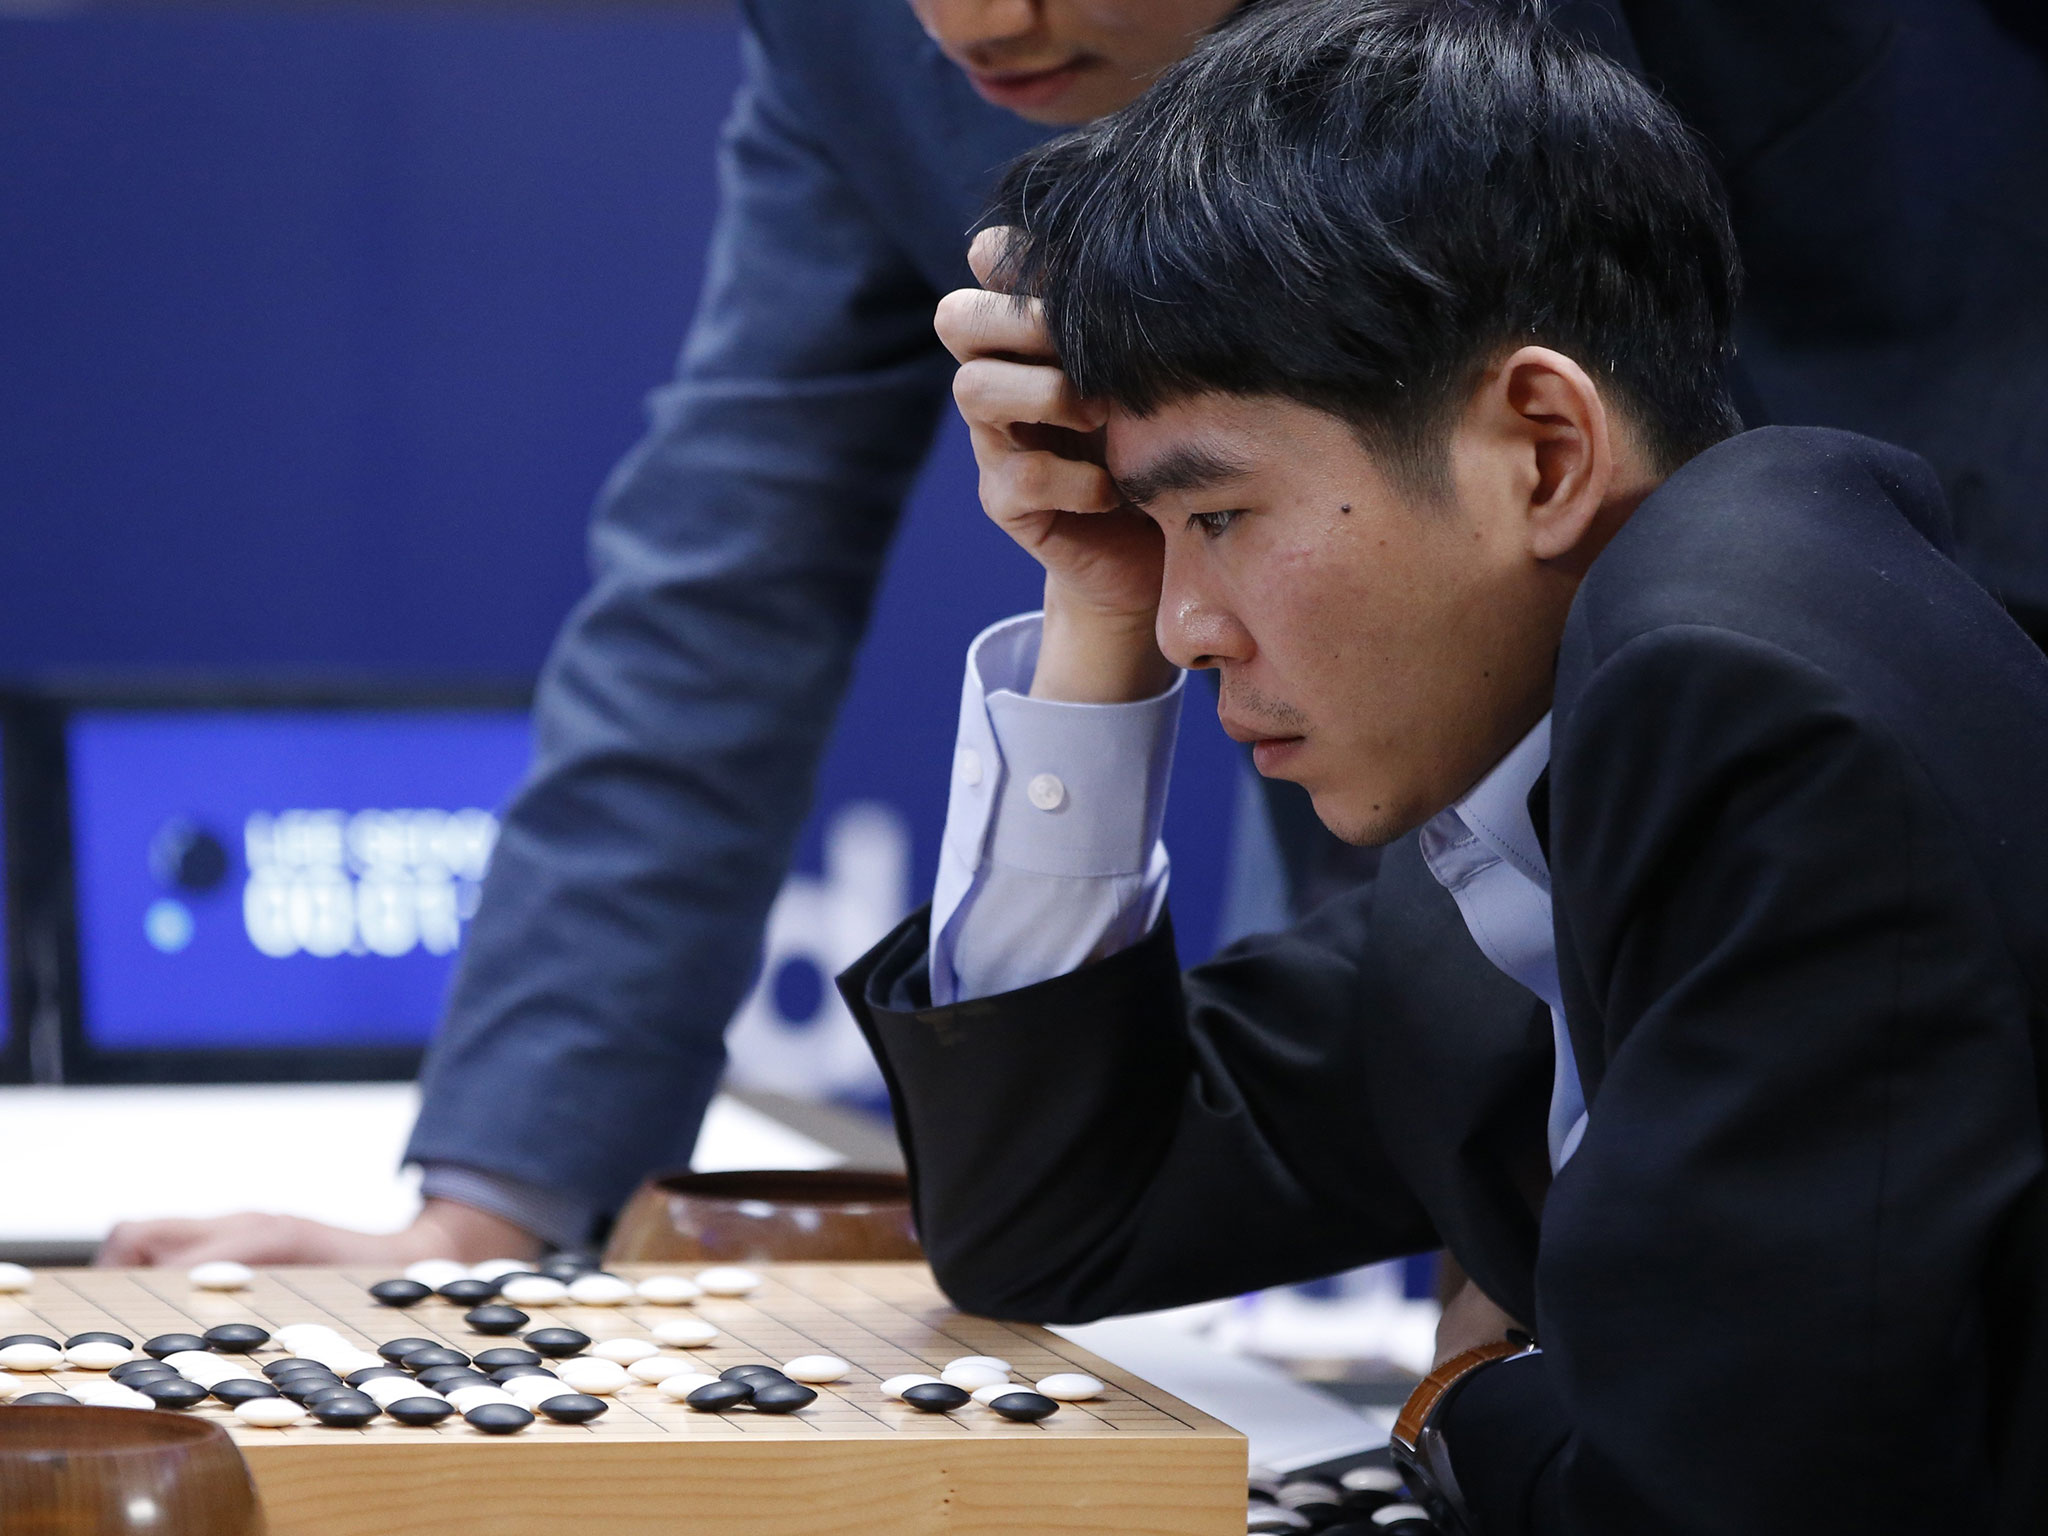
\includegraphics[height=\paperheight]{../img/Lee_Sedol_quotes.jpg}
    }
    \begin{frame}[standout]
      \epigraph{
        \tiny
        I heard Google DeepMind's AI is surprisingly strong and getting stronger, but I am confident that I can win, at least this time.
      }{Lee Sedol}
      \pause

      \epigraph{
        \tiny
        ...even beating AlphaGo by 4:1 may allow the Google DeepMind team to claim its de facto victory and the defeat of him [Lee~Sedol], or even humankind.
      }{interview in JTBC Newsroom}
      \pause
    \end{frame}
  }

  {
    \usebackgroundtemplate{
      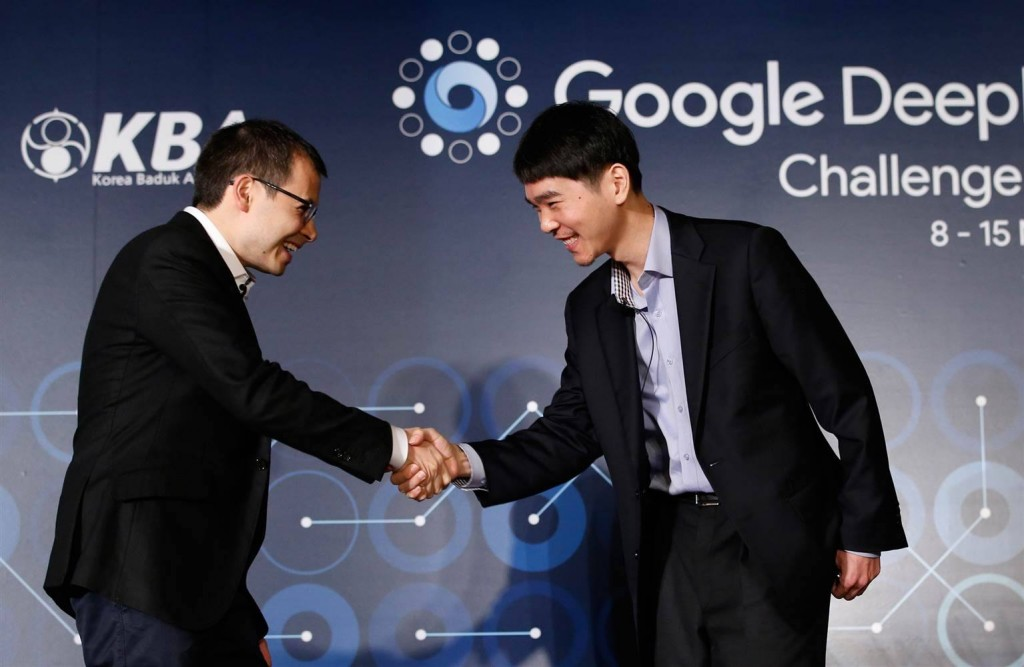
\includegraphics[height=\paperheight]{../img/Lee_Sedol_after_match.jpg}
    }
    \setbeamertemplate{frame footer}{\color{white}\url{https://en.wikipedia.org/wiki/AlphaGo_versus_Lee_Sedol}}
    \begin{frame}{AlphaGo vs. Lee Sedol}
      \pause

      \vskip 1em
      \color{white}
      In March 2016 \textbf{AlphaGo won 4:1} against the legendary Lee Sedol.
      \pause

      AlphaGo won all but the $4^{th}$ game; all games were won by~resignation.
      \pause
    \end{frame}
  }

  {
    \usebackgroundtemplate{
      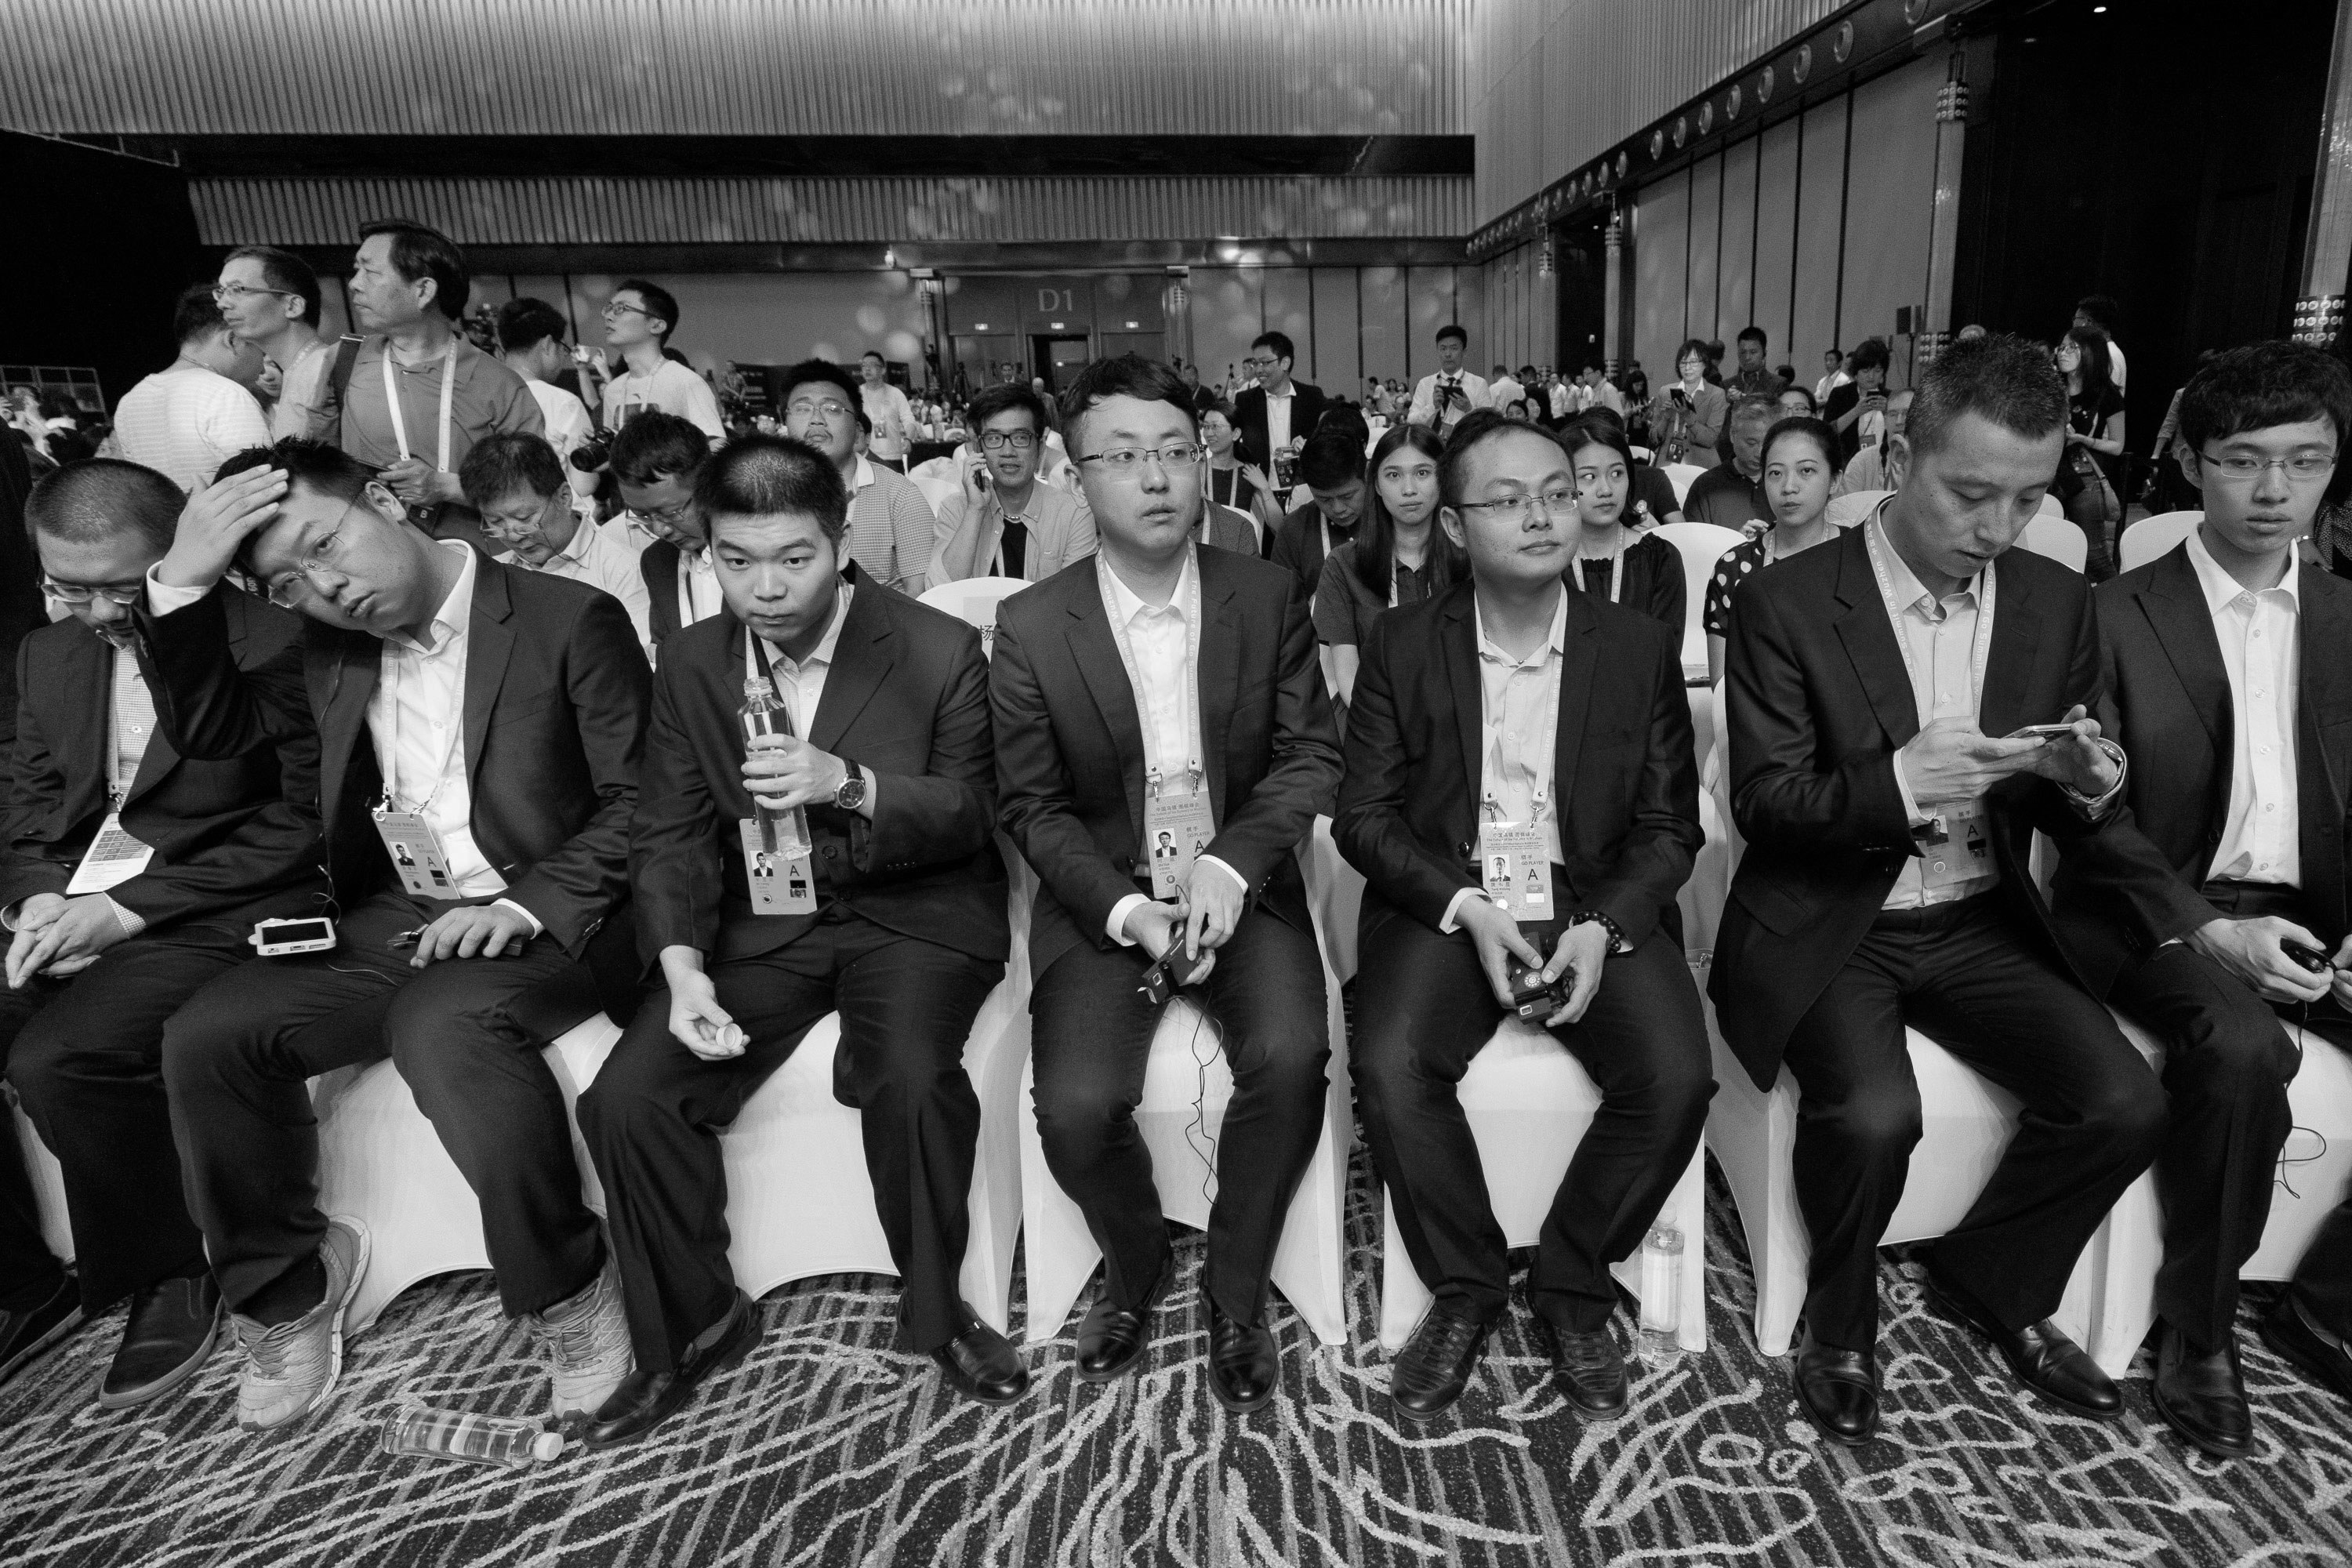
\includegraphics[height=\paperheight]{../img/Go_masters_grayscale.jpg}
    }
    \setbeamertemplate{frame footer}{\color{white}\url{https://deepmind.com/research/alphago/match-archive/master/}}
    \begin{frame}{AlphaGo Master}
      \pause

      \color{white}
      In January 2017, DeepMind revealed that AlphaGo had played a~series of~unofficial online games against some of~the strongest professional Go players under the pseudonyms ``Master'' and ''Magister''.
      \pause

      This AlphaGo was an~improved version of~the AlphaGo that played Lee Sedol in~2016.
      \pause

      Over one week, AlphaGo played 60 online fast time-control games.
      \pause

      \textbf{AlphaGo won this series of games 60:0.}
    \end{frame}
  }

  {
    \setbeamertemplate{frame footer}{\color{black}\url{https://events.google.com/alphago2017/}}

    \usebackgroundtemplate{
      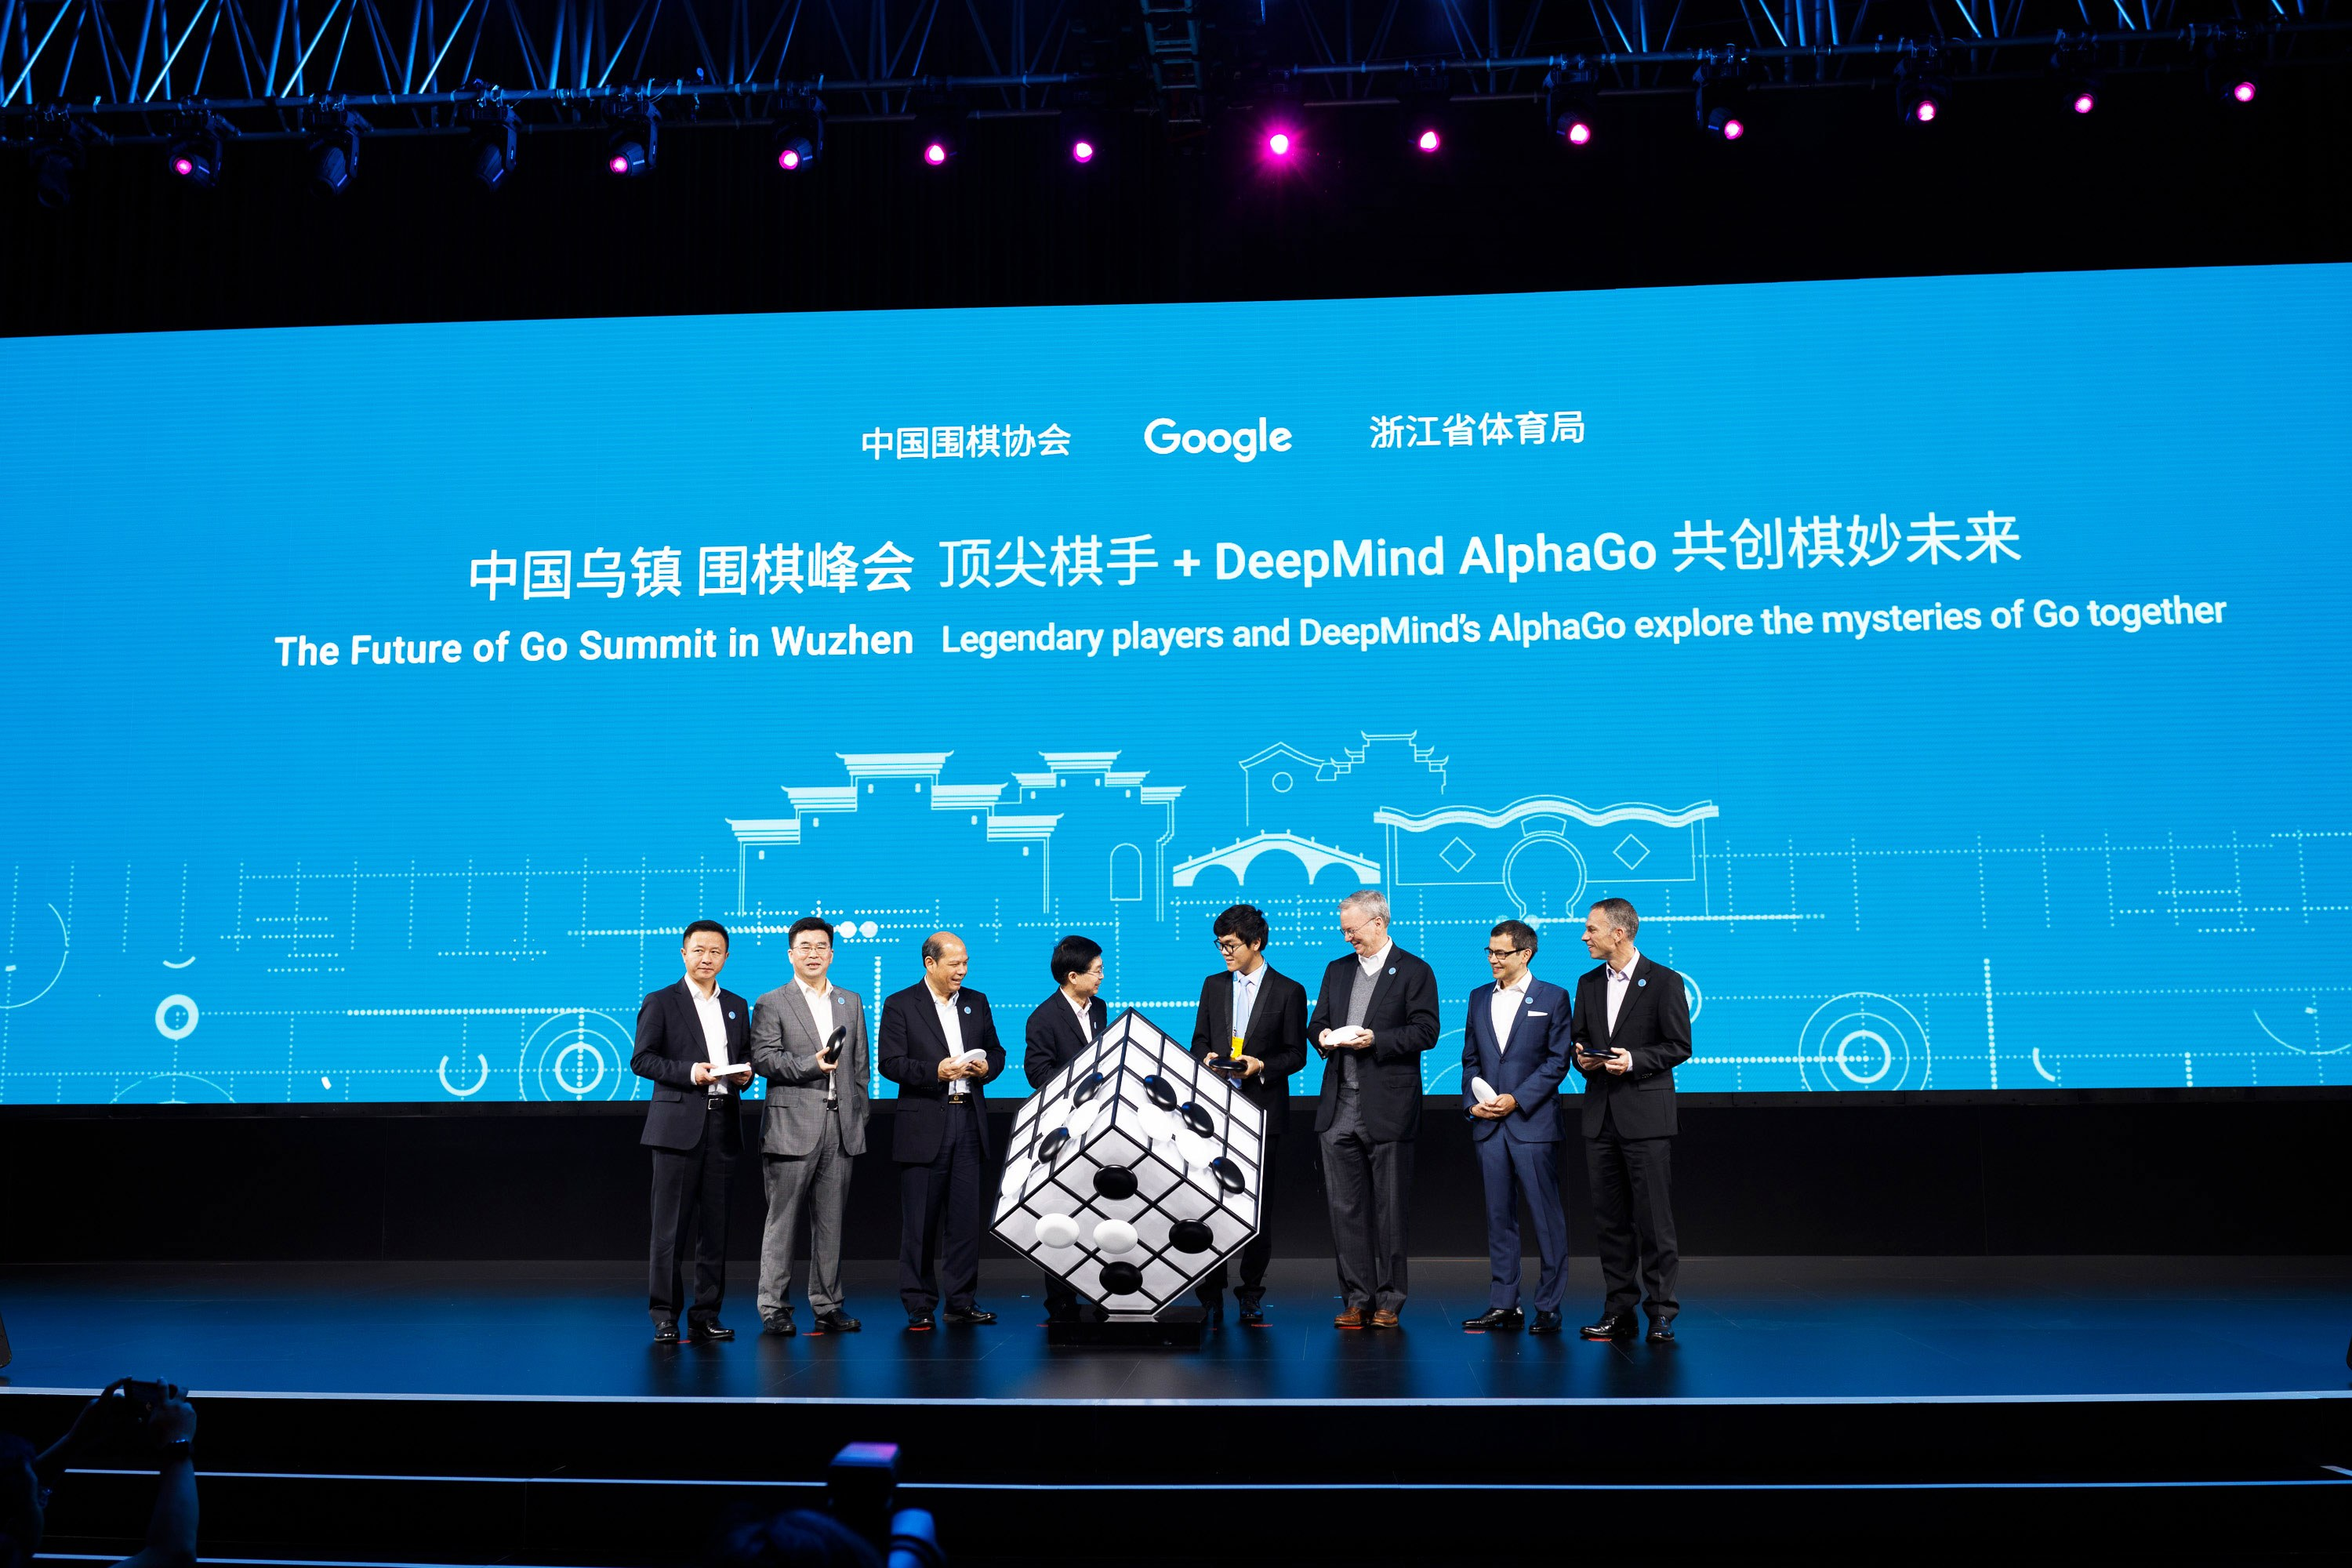
\includegraphics[height=\paperheight]{../img/future_of_Go_summit.jpg}
    }
    \begin{frame}[standout]
    \end{frame}

    \usebackgroundtemplate{
      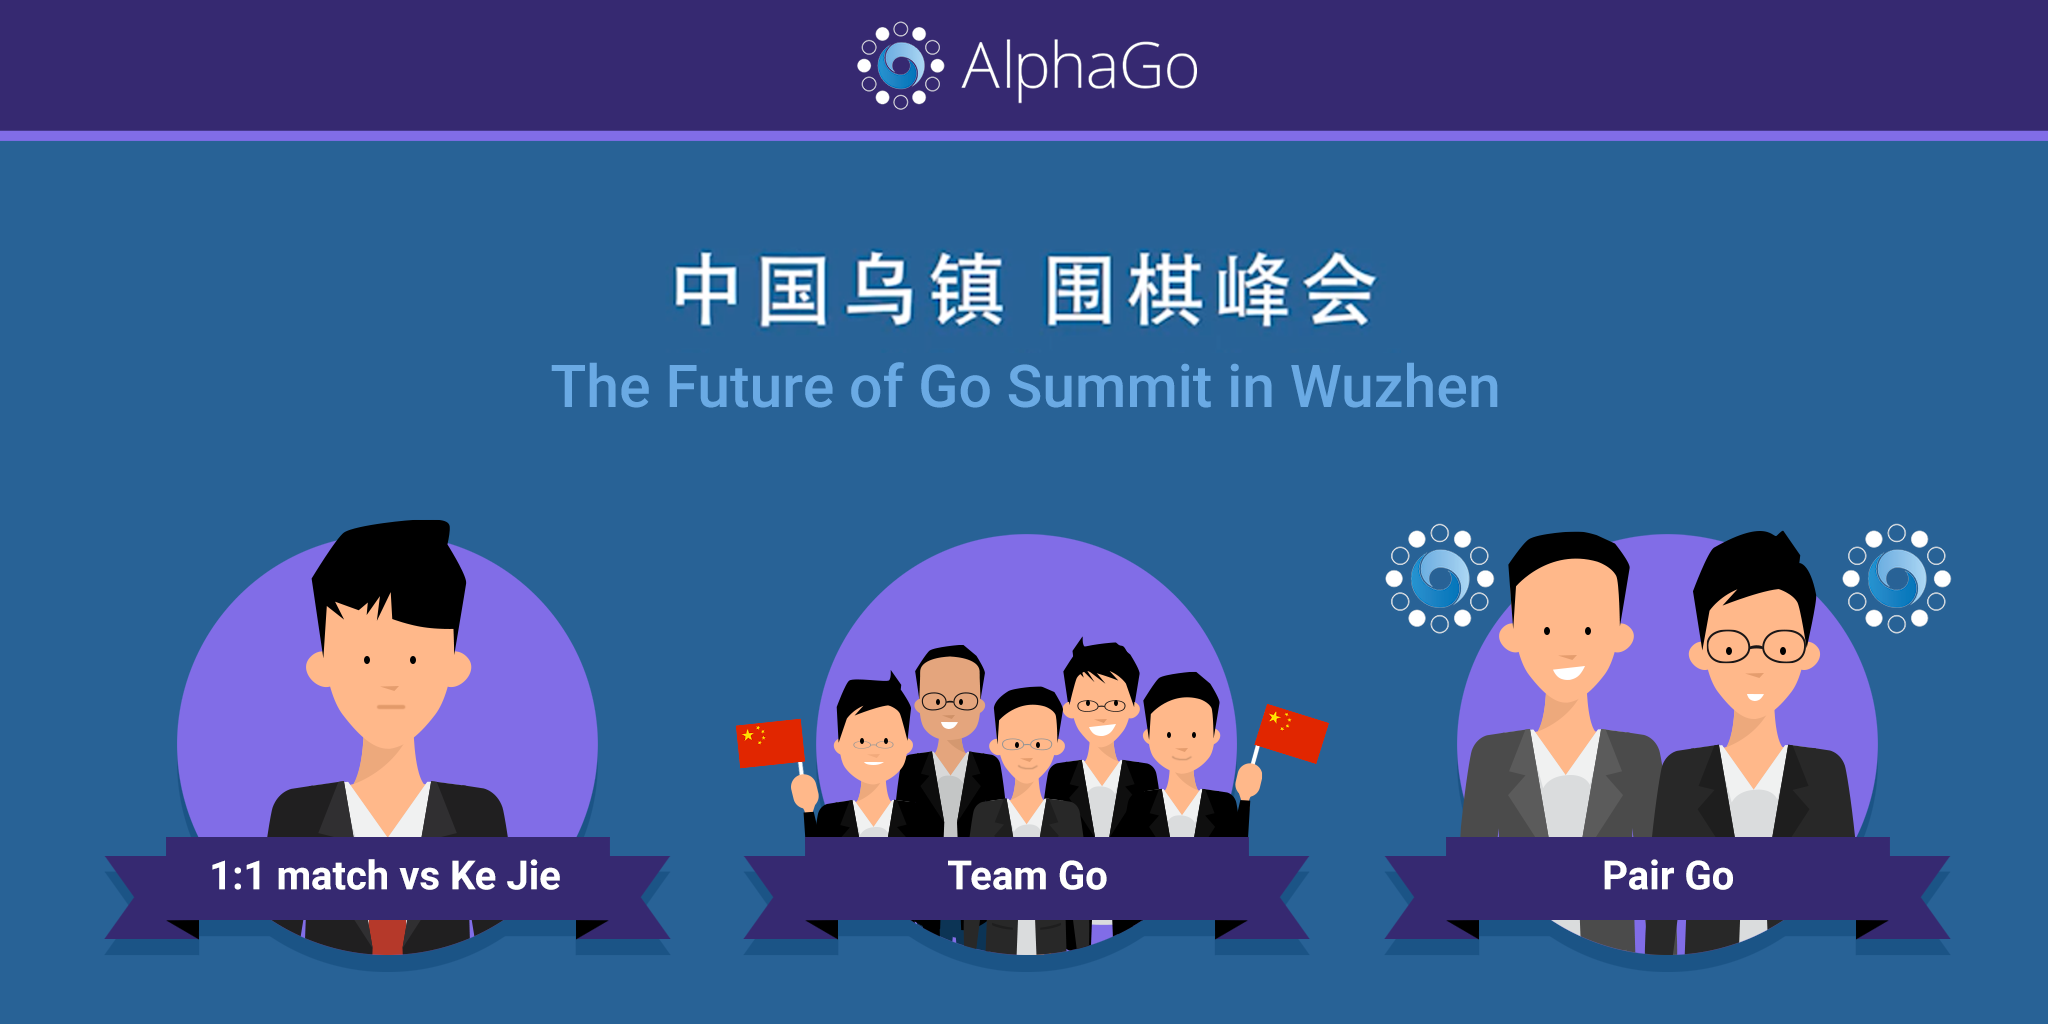
\includegraphics[width=\paperwidth]{../img/future_of_Go_summit_infographics.jpg}
    }
    \begin{frame}
      \vskip .7\textheight

      \pause
      \begin{itemize}[<+- | alert@+>]
        \item 23 May - 27 May 2017 in Wuzhen, China
        \item Team Go vs. AlphaGo \textbf{0:1}
        \item AlphaGo vs. world champion Ke Jie \textbf{3:0}
      \end{itemize}
    \end{frame}
  }

  {
    \usebackgroundtemplate{
      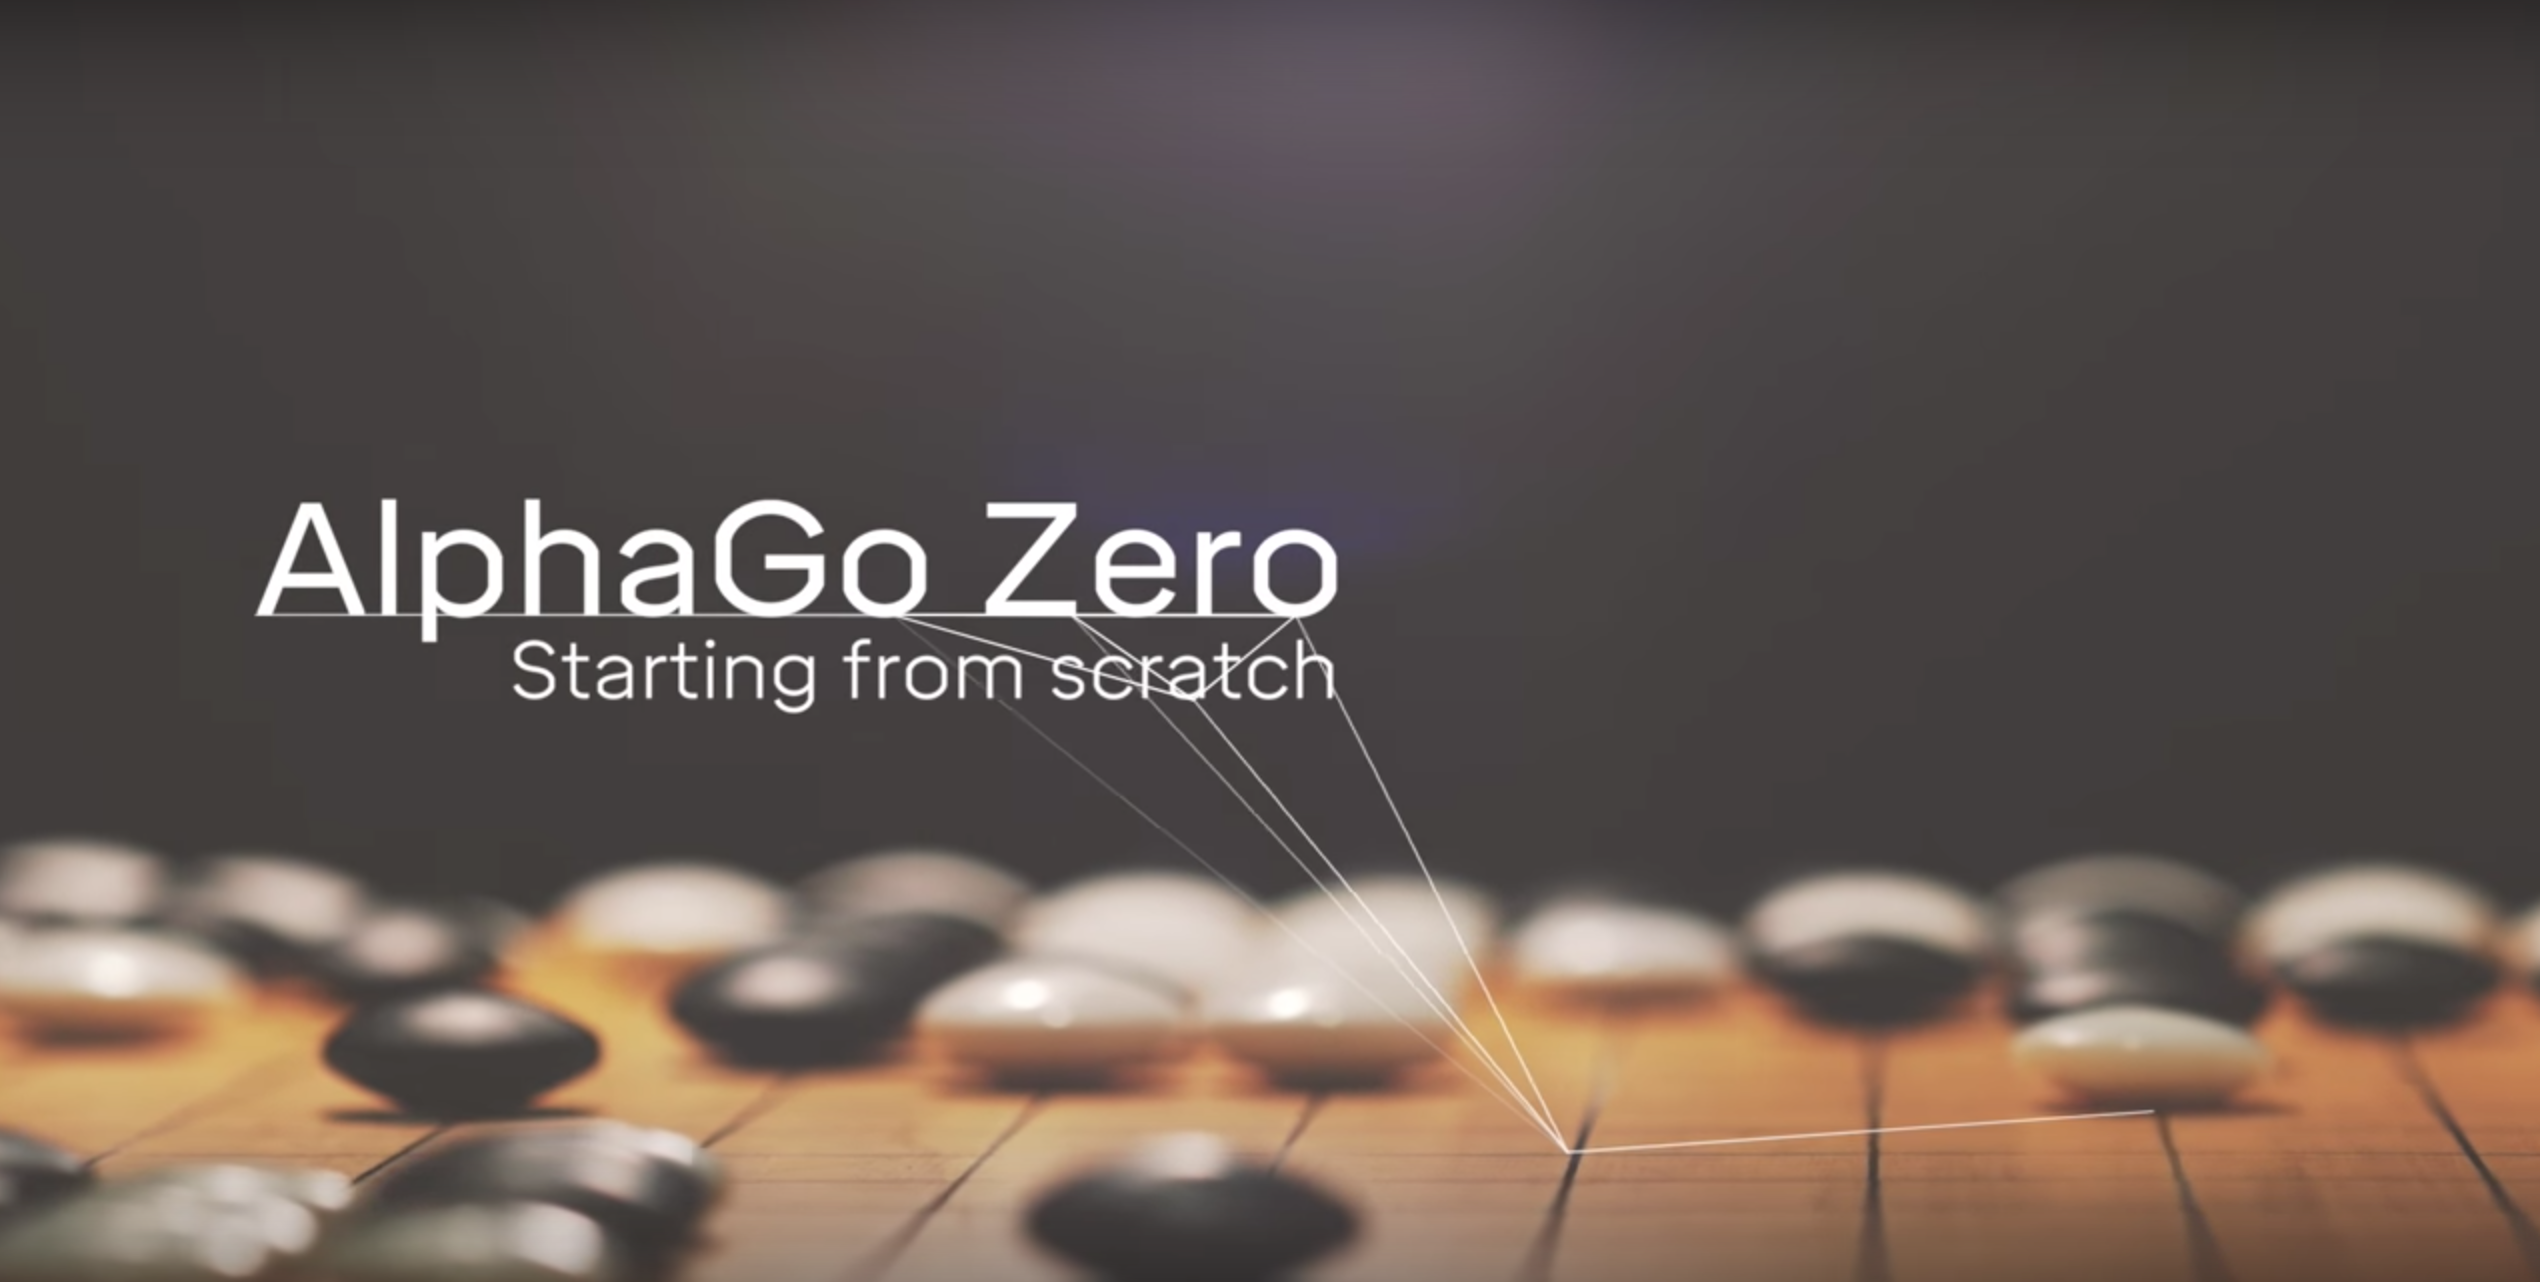
\includegraphics[height=\paperheight]{../img/AlphaGo_Zero.png}
    }
    \begin{frame}[standout]
    \end{frame}
  }

  {
    \usebackgroundtemplate{
      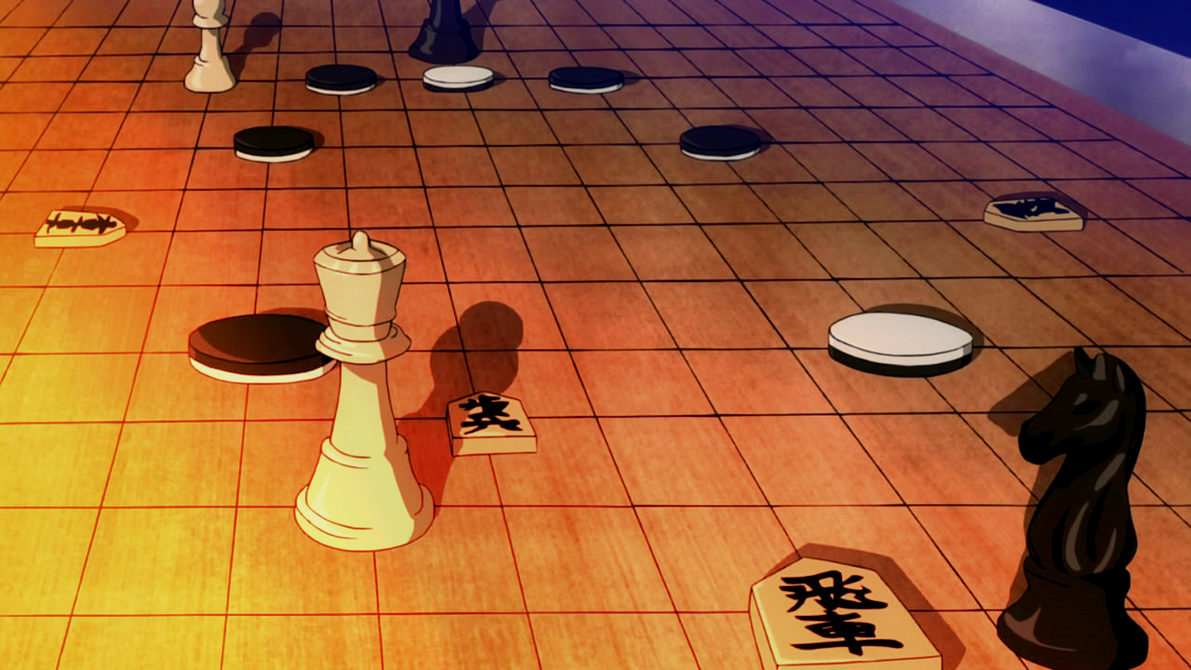
\includegraphics[height=\paperheight]{../img/chess-go-shogi.png}
    }
    \begin{frame}
      \color{black}
      \epigraph{
        AI system that mastered chess, Shogi and Go to ``superhuman levels'' within a~handful of~hours
      }{\Huge AlphaZero}
    \end{frame}
  }

  {
    \usebackgroundtemplate{
      
\includegraphics[height=\paperheight]{../img/deepmind.png}
    }
    \setbeamertemplate{enumerate items}[circle]{\color{white}}
    \begin{frame}[standout]
      \pause
      \begin{enumerate}[<+- | alert@+>]
        \item AlphaGo Fan
        \item AlphaGo Lee
        \item AlphaGo Master
        \item AlphaGo Zero
        \item AlphaZero
      \end{enumerate}
    \end{frame}
  }

%%%%%%%%%%%%%%%%%%%%%%%%%%%%%%%%%%%%%%%%%%%%%%%%%%%%%%%%%%%%%%%%%%%%%%%%%%%%%%%%

  \section{AlphaGo}
  {
    \setbeamertemplate{frame footer}{[\cite{Silver2016mastering}]}

    \begin{frame}{Policy and Value Networks}
      \begin{center}
        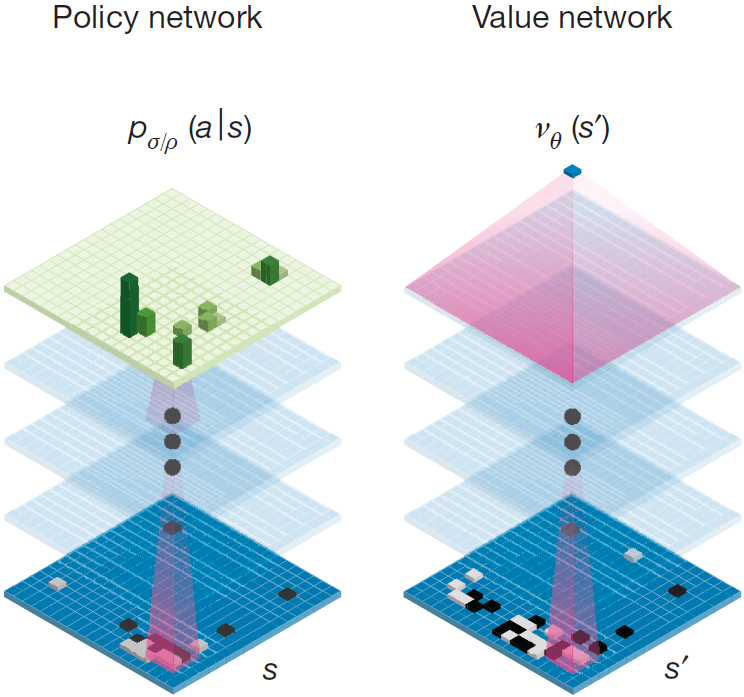
\includegraphics[height=.85\textheight]{../img/policy_and_value_network.png}
      \end{center}
    \end{frame}

    \begin{frame}{Training the (Deep Convolutional) Neural Networks}
      \begin{center}
        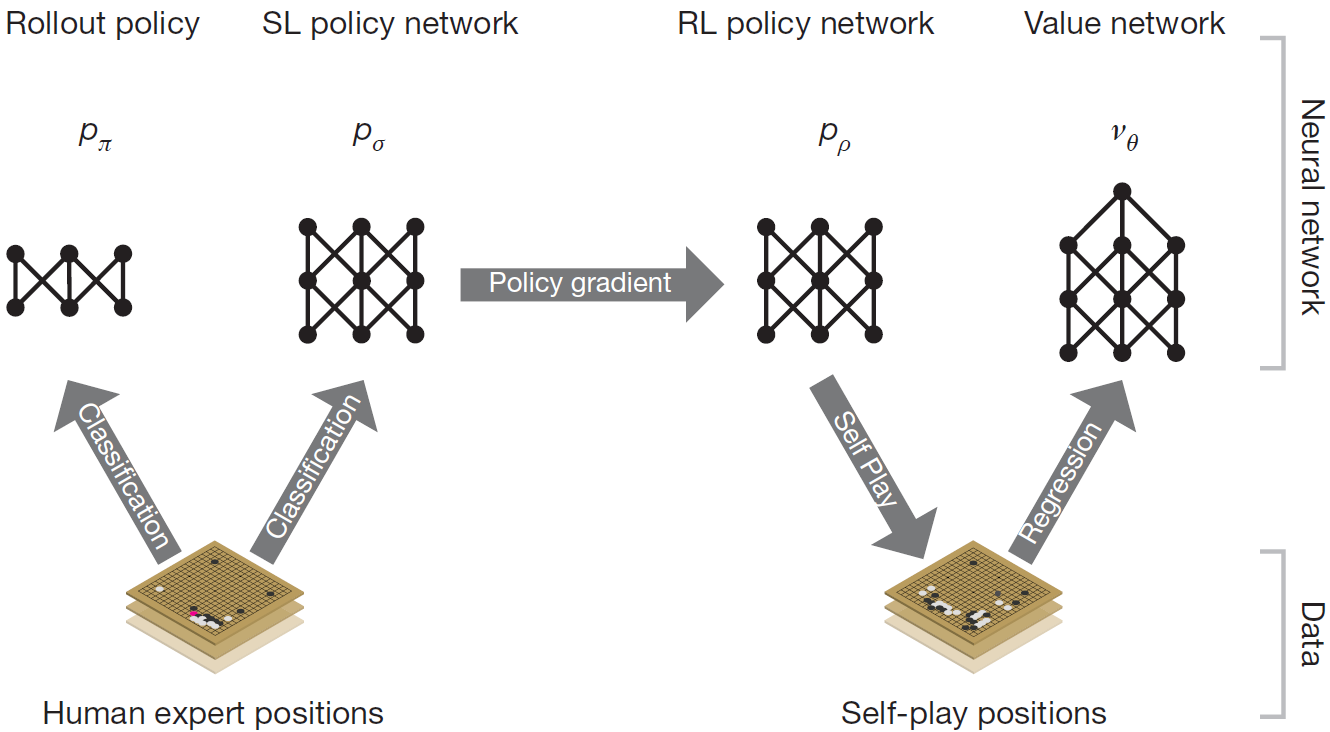
\includegraphics[width=\textwidth]{../img/neural_nets_pipeline.png}
      \end{center}
    \end{frame}
  }

%%%%%%%%%%%%%%%%%%%%%%%%%%%%%%%%%%%%%%%%%%%%%%%%%%%%%%%%%%%%%%%%%%%%%%%%%%%%%%%%

  \section{AlphaGo Zero (AG0)}
  {
    \setbeamertemplate{frame footer}{[\cite{Silver2017AlphaGoZero}]}

    \begin{frame}{AG0: Differences Compared to AlphaGo \{Fan, Lee, Master\}}
      AlphaGo \{Fan, Lee, Master\} $\times$ \alert{AlphaGo Zero}:
      \pause
      \begin{itemize}[<+->]
        \item supervised learning from human expert positions $\times$ \alert{from scratch by self-play reinforcement learning (``tabula rasa'')}
        \item additional (auxialiary) input features $\times$ \alert{only the black and white stones from the board as input features}
        \item separate policy and value networks $\times$ \alert{single neural network}
        \item tree search using also Monte Carlo rollouts $\times$ \alert{simpler tree search using only the single neural network to both evaluate positions and sample moves}
      \end{itemize}
      \pause

      AG0 achieves this via
      \begin{itemize}[<+->]
        \item a~new \alert{reinforcement learning} algorithm
        \item with \alert{lookahead search inside the training loop}
      \end{itemize}
    \end{frame}

    \begin{frame}{AG0: Self-Play Reinforcement Learning}
      \pause
      \begin{center}
        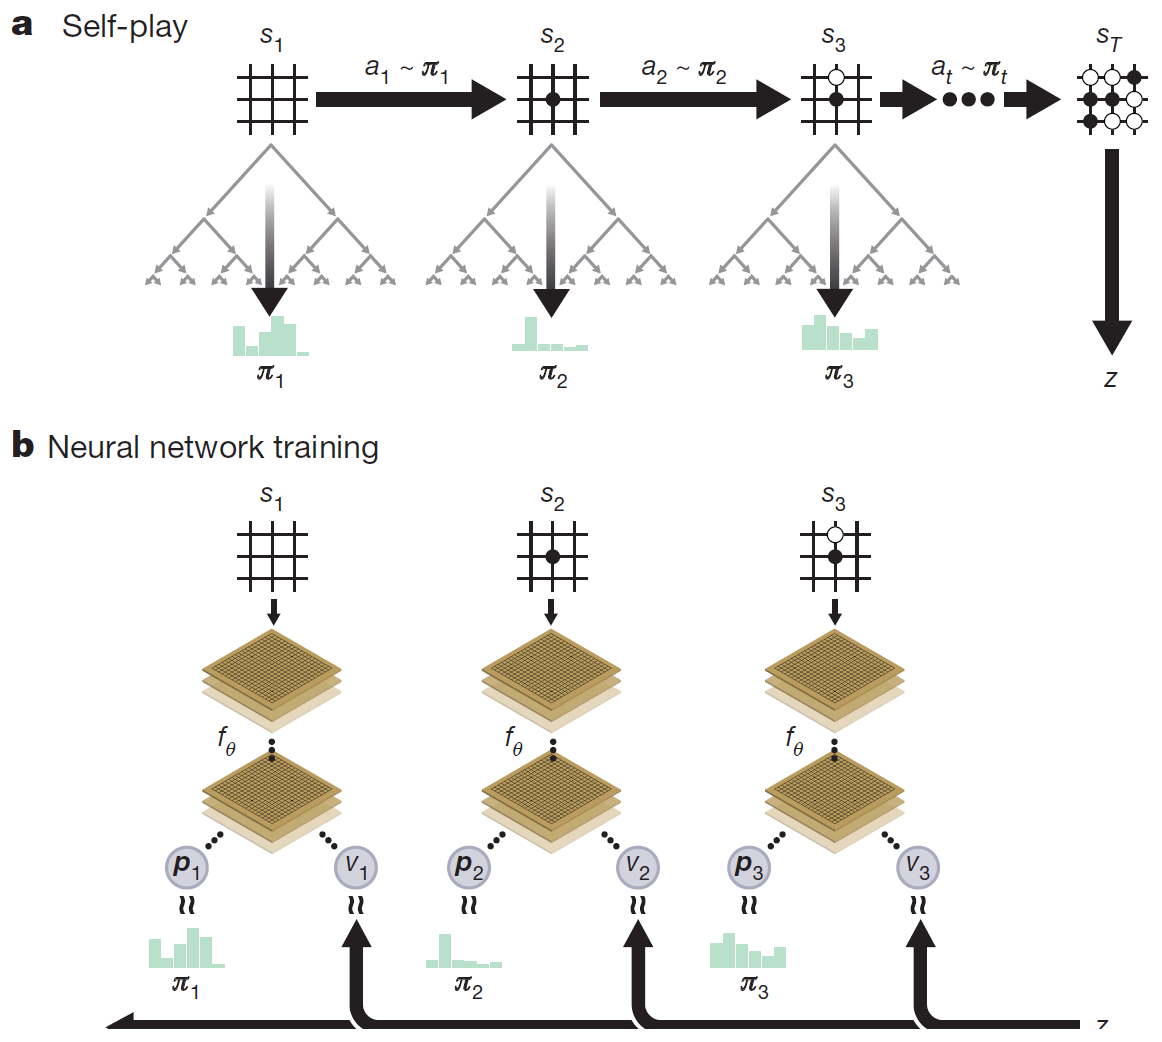
\includegraphics[height=.9\textheight]{../img/AG0-paper/self-play-RL-in-AG0.png}
      \end{center}
    \end{frame}

    \begin{frame}{AG0: Self-Play Reinforcement Learning -- Neural Network}
      deep neural network $f_\theta$ with parameters~$\theta$:
      \pause
      \begin{itemize}[<+- | alert@+>]
        \item input: raw board representation~$s$
        \item output:
          \begin{itemize}[<+- | alert@+>]
            \item move probabilities $\p$
            \item value $v$ of~the board position
            \item $f_\theta(s) = (\p, v)$
          \end{itemize}
        \item specifics:
          \begin{itemize}[<+- | alert@+>]
            \item (20 or 40) residual blocks (of convolutional layers)
            \item batch normalization
            \item rectifier non-linearities
          \end{itemize}
      \end{itemize}
    \end{frame}

    \begin{frame}{AG0: Self-Play Reinforcement Learning -- Steps}
      \begin{enumerate}[<+- | alert@+>]
        \item[0.] random weights $\theta_0$
        \item at each iteration $i > 0$, self-play games are generated:
          \begin{enumerate}[<+- | alert@+>]
            \item[i.] MCTS samples search probabilities $\mathbf{\pi}_t$ based on the neural network from the previous iteration $f_{\theta_{i-1}}$:
              $$\mathbf{\pi}_t = \alpha_{\theta_{i-1}}(s_t)$$
              for each time-step $t = 1, 2, \ldots, T$
            \item[ii.] move is sampled from $\mathbf{\pi}_t$
            \item[iii.] data $(s_t, \mathbf{\pi}_t, z_t)$ for each $t$ are stored for later training
            \item[iv.] new neural network $f_{\theta_{i}}$ is trained in order to minimize the loss
              $$l = (z - v)^2 - \mathbf{\pi}^\top \log \p + c || \theta ||^2$$
          \end{enumerate}
      \end{enumerate}
      \pause
      \vskip -2em
      Loss~$l$ makes $(\p, v) = f_\theta(s)$ more closely match the improved search probabilities and self-play winner $(\mathbf{\pi}, z)$.
    \end{frame}

    \begin{frame}{AG0: Self-Play Reinforcement Learning -- Review}
      \begin{center}
        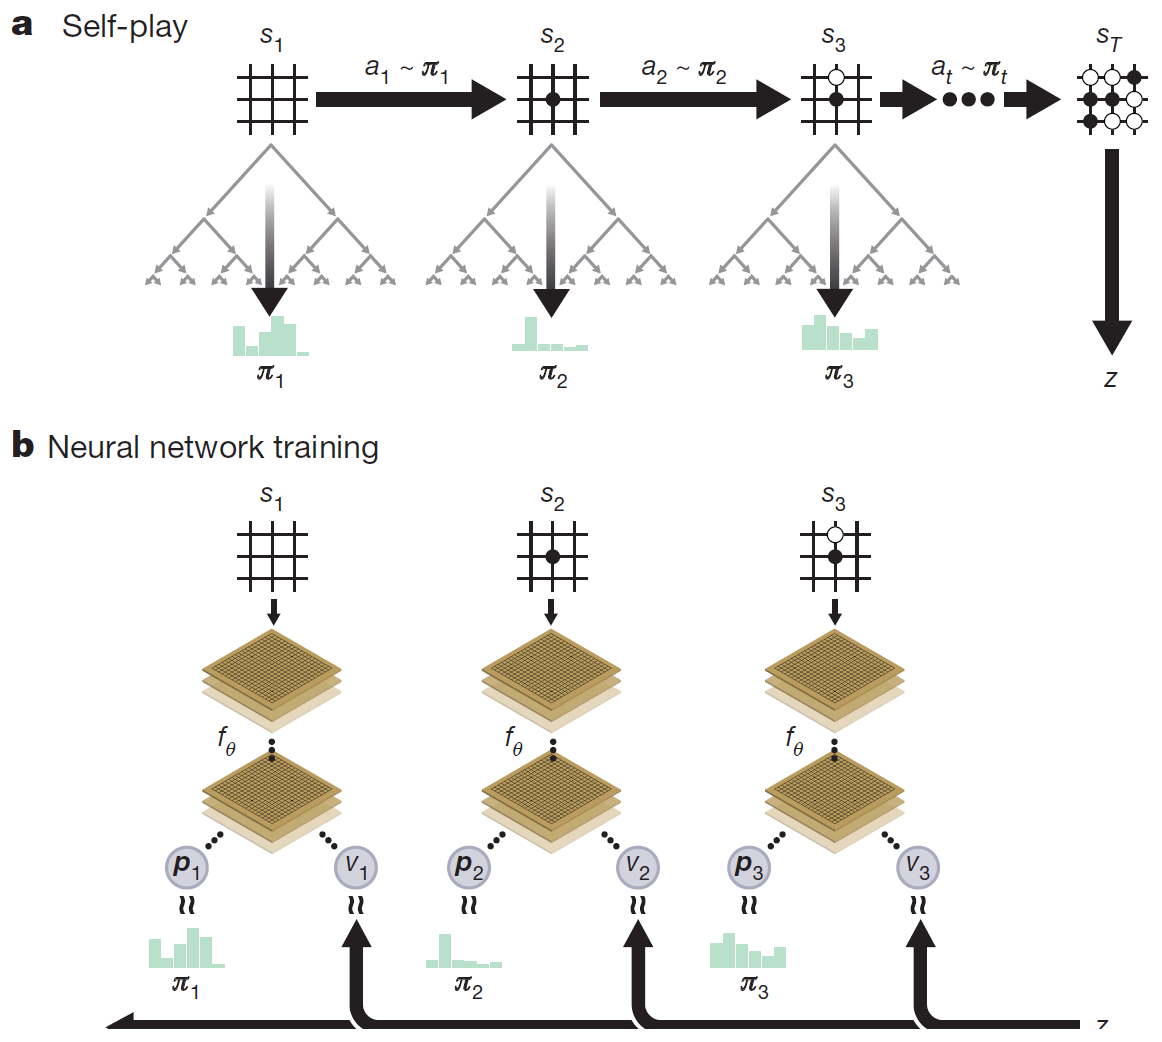
\includegraphics[height=.9\textheight]{../img/AG0-paper/self-play-RL-in-AG0.png}
      \end{center}
    \end{frame}

    \begin{frame}{AG0: Elo Rating over Training Time (RL vs. SL)}
      \begin{center}
        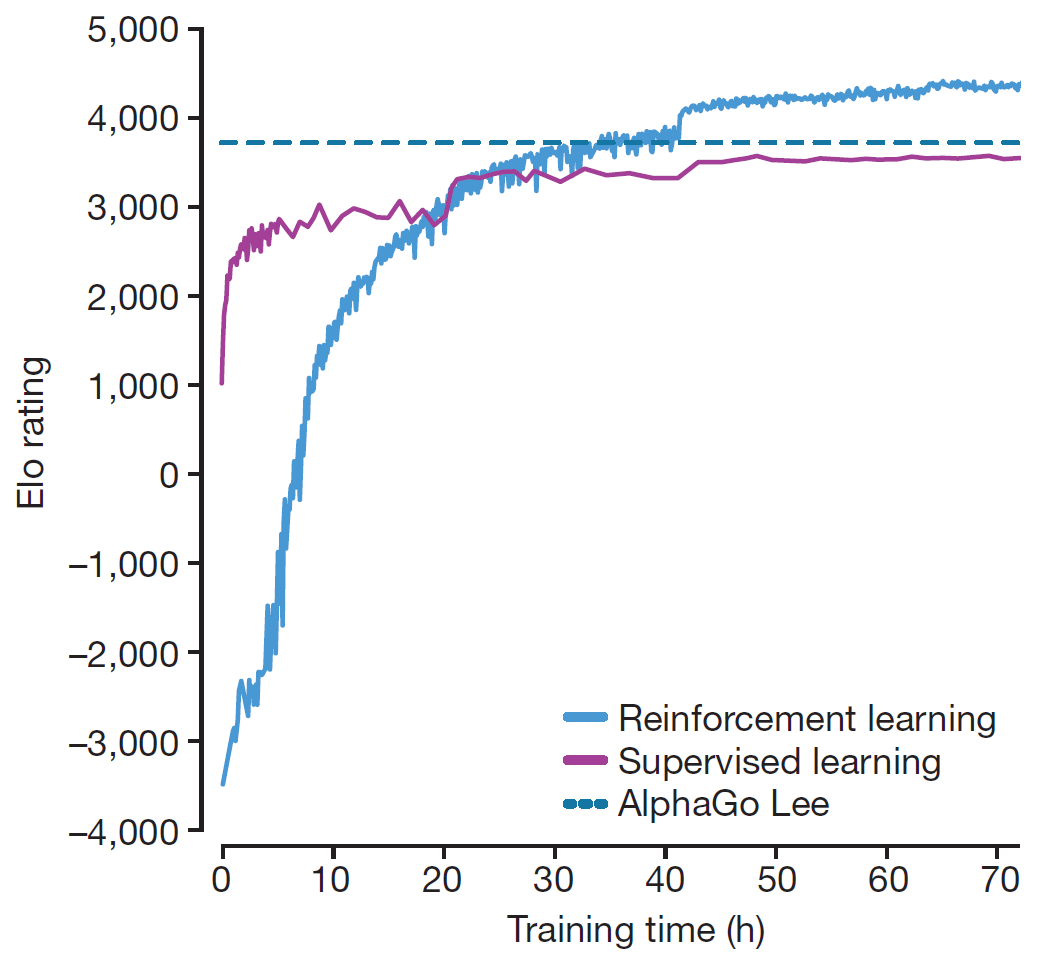
\includegraphics[height=.9\textheight]{../img/AG0-paper/training-time-vs-elo.png}
      \end{center}
    \end{frame}

    \begin{frame}{AG0: Monte Carlo Tree Search (1/2)}
      Monte Carlo Tree Search (MCTS) in AG0:
      \pause

      \begin{center}
        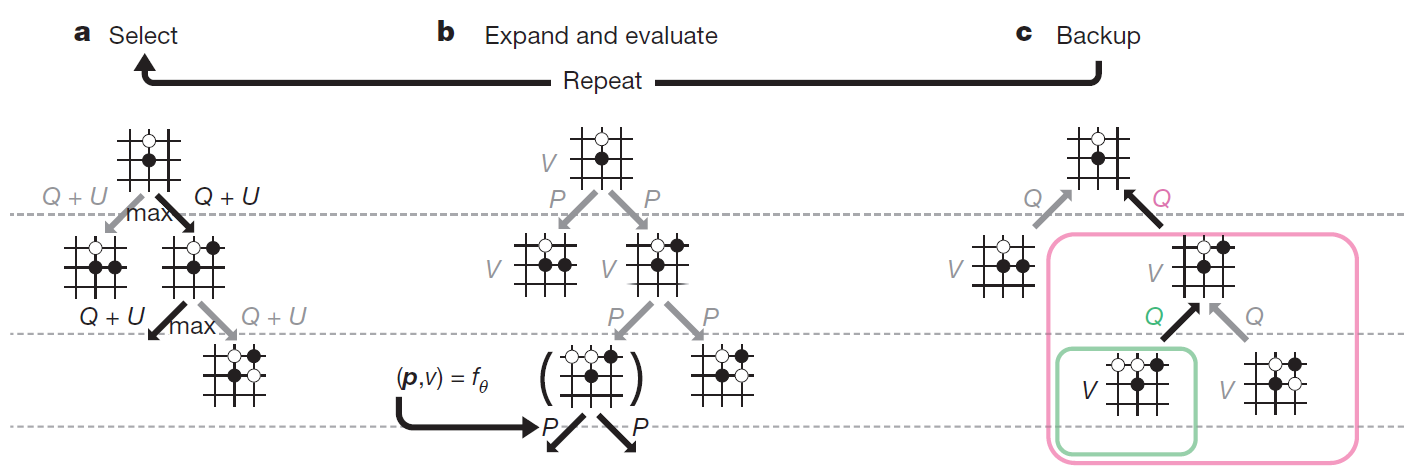
\includegraphics[width=\textwidth]{../img/AG0-paper/MCTS-1.png}
      \end{center}
    \end{frame}

    \begin{frame}{AG0: Monte Carlo Tree Search (2/2)}
      \begin{center}
        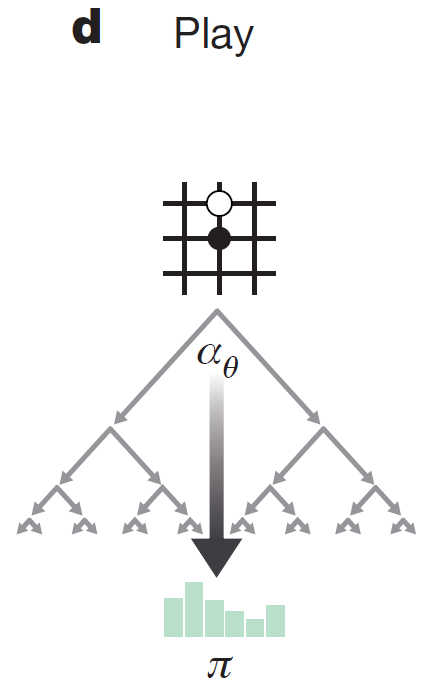
\includegraphics[height=.85\textheight]{../img/AG0-paper/MCTS-2.png}
      \end{center}
    \end{frame}

    \begin{frame}{AG0: Elo Rating over Training Time (AG0 with 40 blocks)}
      \begin{center}
        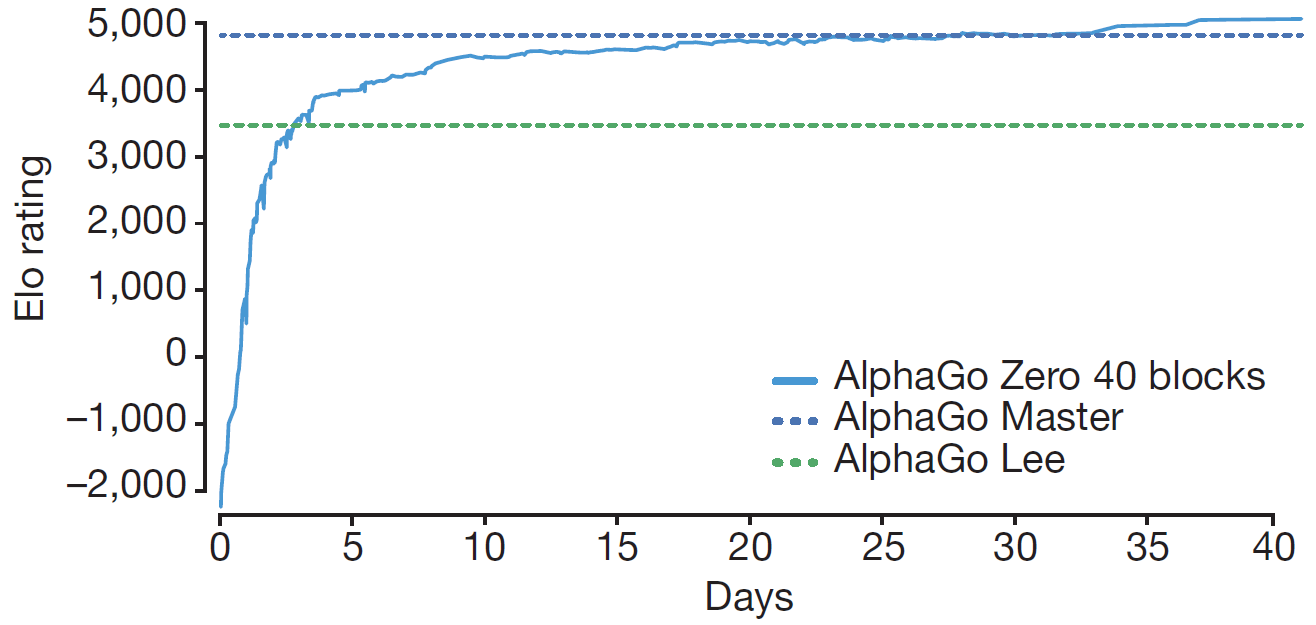
\includegraphics[width=\textwidth]{../img/AG0-paper/AG0-40-elo-vs-training-days.png}
      \end{center}
    \end{frame}

    \begin{frame}{AG0: Tournament between AI Go Programs}
      \begin{center}
        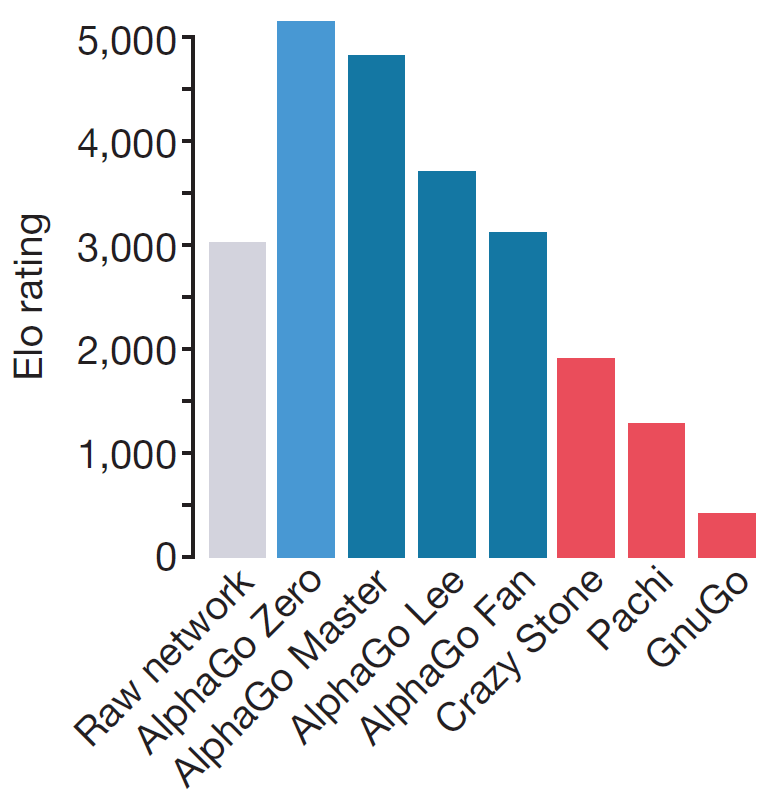
\includegraphics[height=.9\textheight]{../img/AG0-paper/elo-from-tournament.png}
      \end{center}
    \end{frame}

    \begin{frame}{AG0: Comparison of Various Neural Network Architectures}
      \begin{center}
        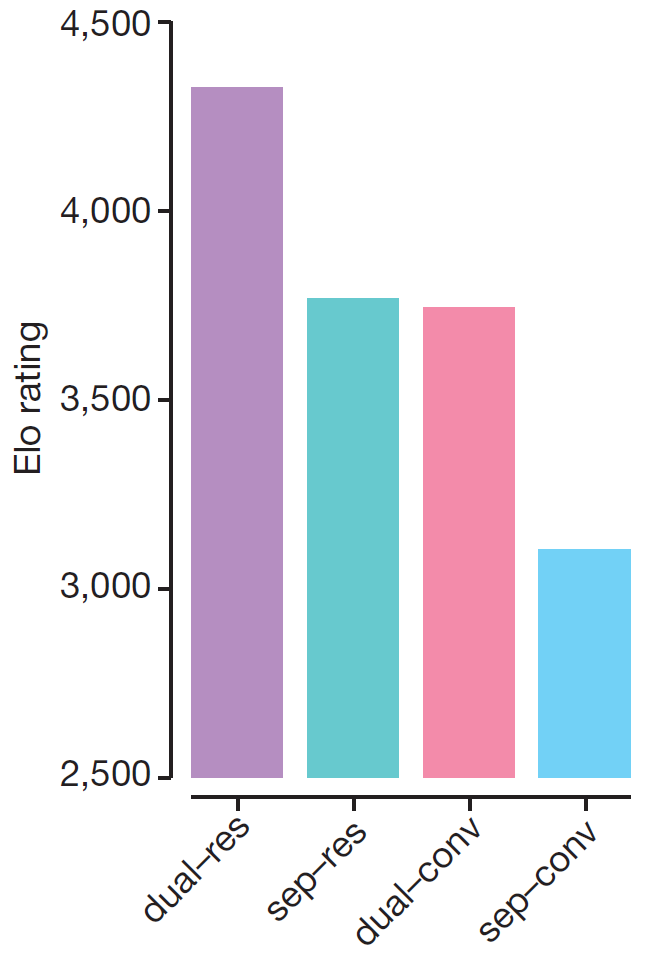
\includegraphics[height=.9\textheight]{../img/AG0-paper/nn-arch-vs-elo.png}
      \end{center}
    \end{frame}

    \begin{frame}{AG0: Discovered Joseki (Corner Sequences)}
      \begin{center}
        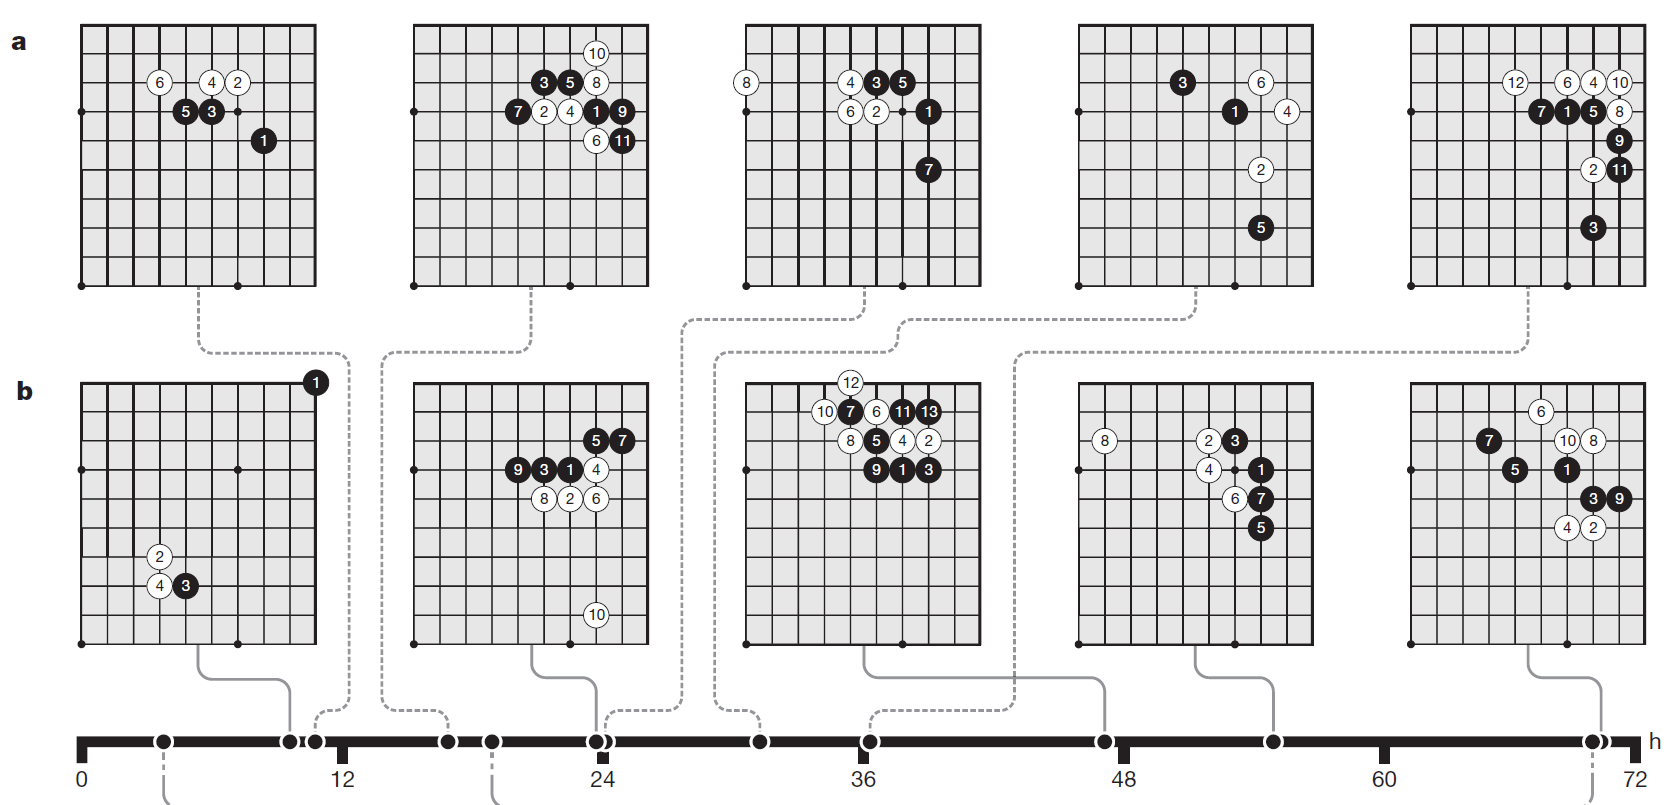
\includegraphics[width=\textwidth]{../img/AG0-paper/discovered-openings.png}
      \end{center}
      \pause

      \begin{description}[<+- | alert@+>]
        \item[a] five human \textit{joseki}
        \item[b] five novel \textit{joseki} variants eventually preferred by AG0
      \end{description}
    \end{frame}

    \begin{frame}{AG0: Discovered Playing Styles}
      \begin{center}
        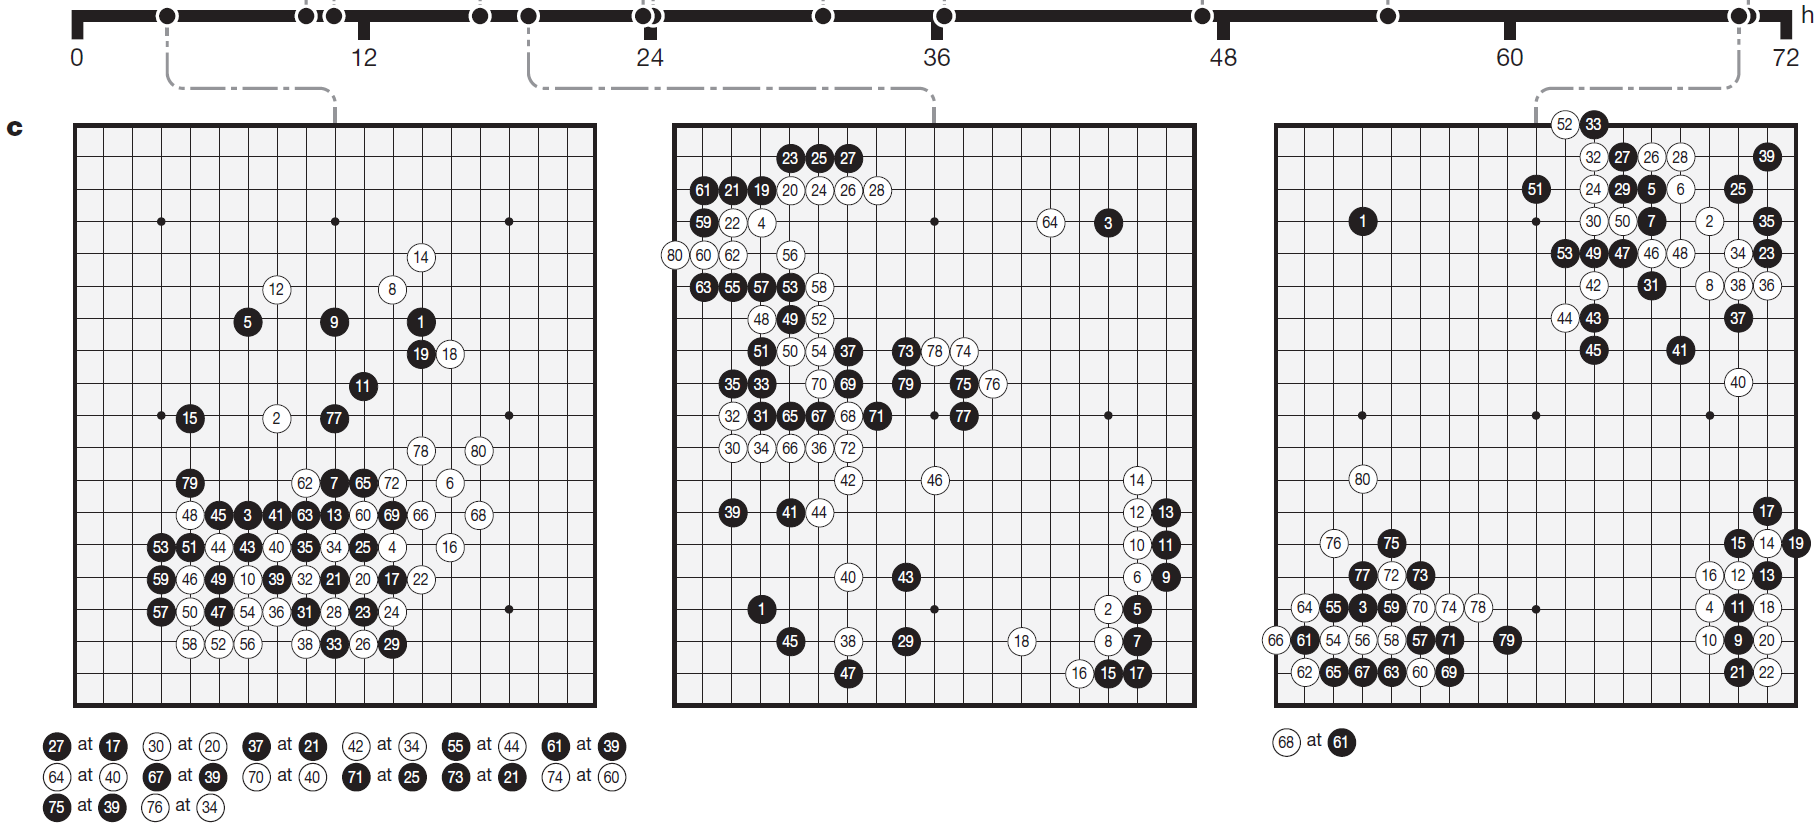
\includegraphics[width=\textwidth]{../img/AG0-paper/playing-styles-discovered-in-time.png}
      \end{center}
      \pause

      \vskip -.5cm
      \begin{description}[<+- | alert@+>]
        \item[at 3 h] greedy capture of stones
        \item[at 19 h] the fundamentals of Go concepts (life-and-death, influence, territory...)
        \item[at 70 h] remarkably balanced game (multiple battles, complicated \textit{ko} fight, a~half-point win for white...)
      \end{description}
    \end{frame}
  }

%%%%%%%%%%%%%%%%%%%%%%%%%%%%%%%%%%%%%%%%%%%%%%%%%%%%%%%%%%%%%%%%%%%%%%%%%%%%%%%%

  \section{AlphaZero}
  {
    \usebackgroundtemplate{
      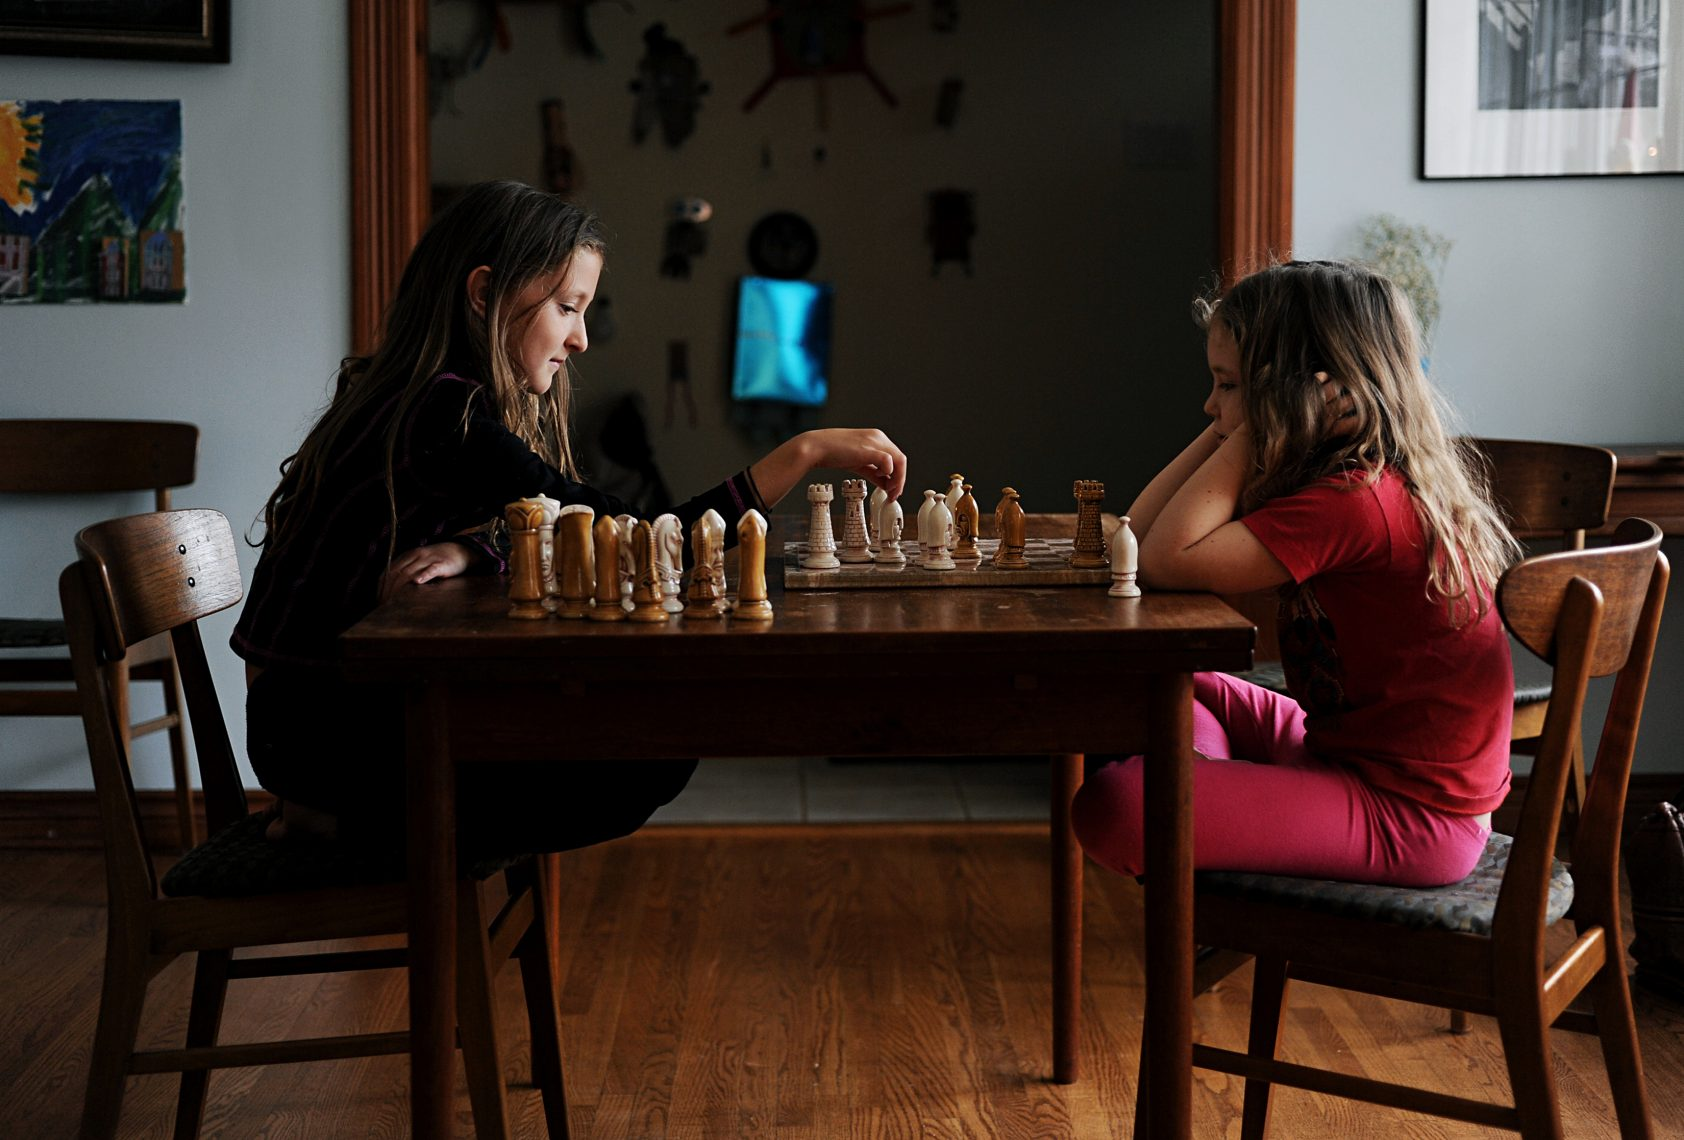
\includegraphics[height=\paperheight]{../img/girls_playing_chess.jpg}
    }
    \begin{frame}[standout]
      \pause
      \vskip .5\textheight

      \epigraph{
        \tiny
        To watch such a~strong programme like Stockfish, against whom most top players would be happy to win even one game out of a~hundred, being completely taken apart is certainly definitive.
      }{Viswanathan Anand}

      \pause
      \epigraph{
        \tiny
        It’s like chess from another dimension.
      }{Demis Hassabis}
    \end{frame}
  }

  {
    \setbeamertemplate{frame footer}{[\cite{Silver2017AlphaZero}]}

    \begin{frame}{AlphaZero: Differences Compared to AlphaGo Zero}
      AlphaGo Zero $\times$ \alert{AlphaZero}:
      \pause
      \begin{itemize}[<+->]
        \item binary outcome (win / loss) $\times$ \alert{expected outcome (including draws or potentially other outcomes)}
        \item board positions transformed before passing to neural networks (by randomly selected rotation or reflection) $\times$ \alert{no data augmentation}
        \item games generated by the best player from previous iterations (margin of 55~\%) $\times$ \alert{continual update using the latest parameters (without the evaluation and selection steps)}
        \item hyper-parameters tuned by Bayesian optimisation $\times$ \alert{reused the same hyper-parameters without game-specific tuning}
      \end{itemize}
    \end{frame}

    \begin{frame}{AlphaZero: Openings Discovered by the Self-Play (1/2)}
      \begin{center}
        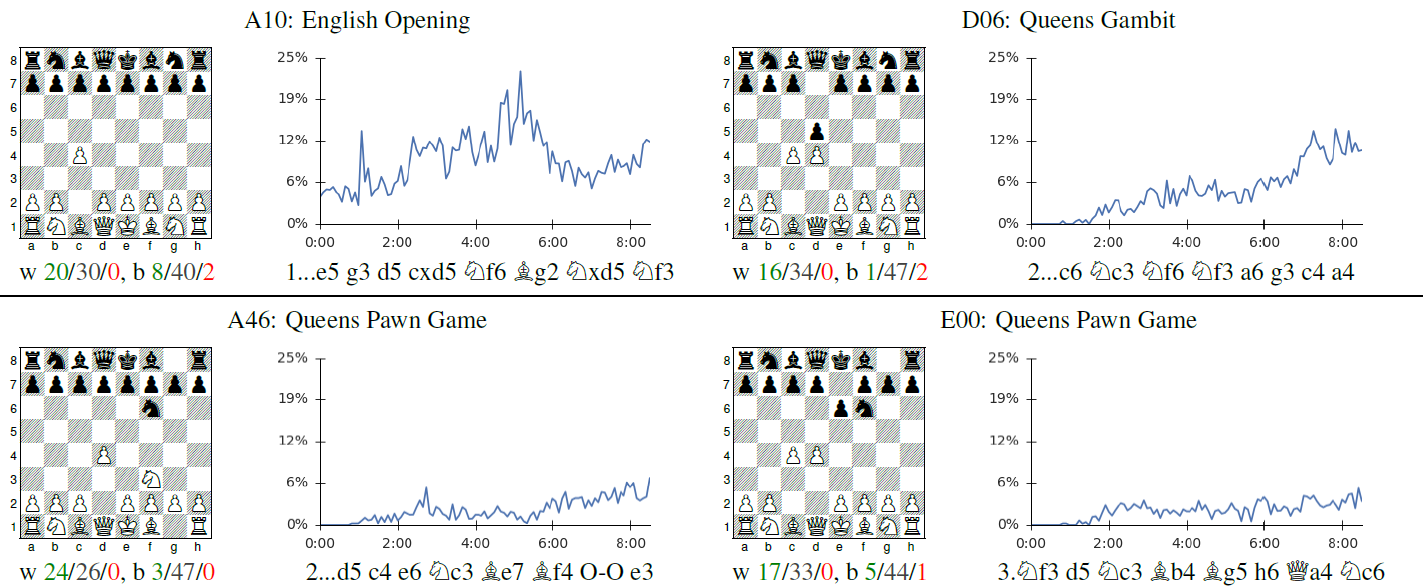
\includegraphics[width=\textwidth]{../img/AlphaZero-paper/openings-1.png}
      \end{center}
    \end{frame}

    \begin{frame}{AlphaZero: Openings Discovered by the Self-Play (2/2)}
      \begin{center}
        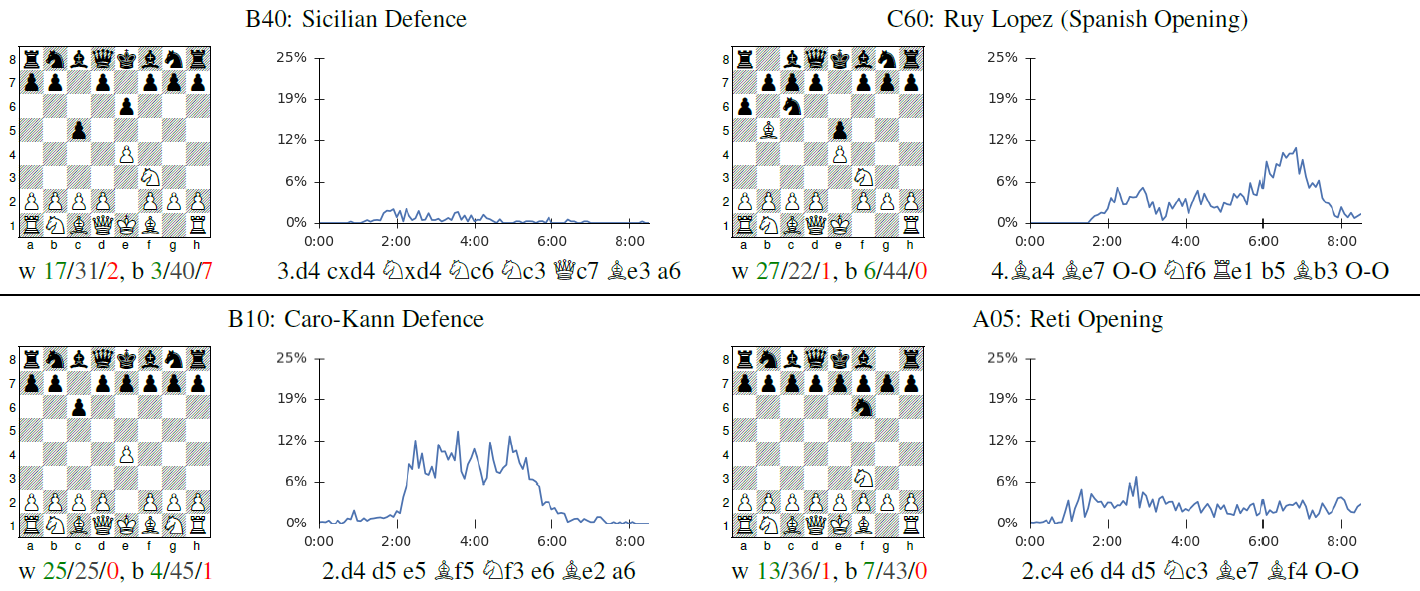
\includegraphics[width=\textwidth]{../img/AlphaZero-paper/openings-2.png}
      \end{center}
    \end{frame}

    \begin{frame}{AlphaZero: Elo Rating over Training Time}
      \begin{center}
        \pause
        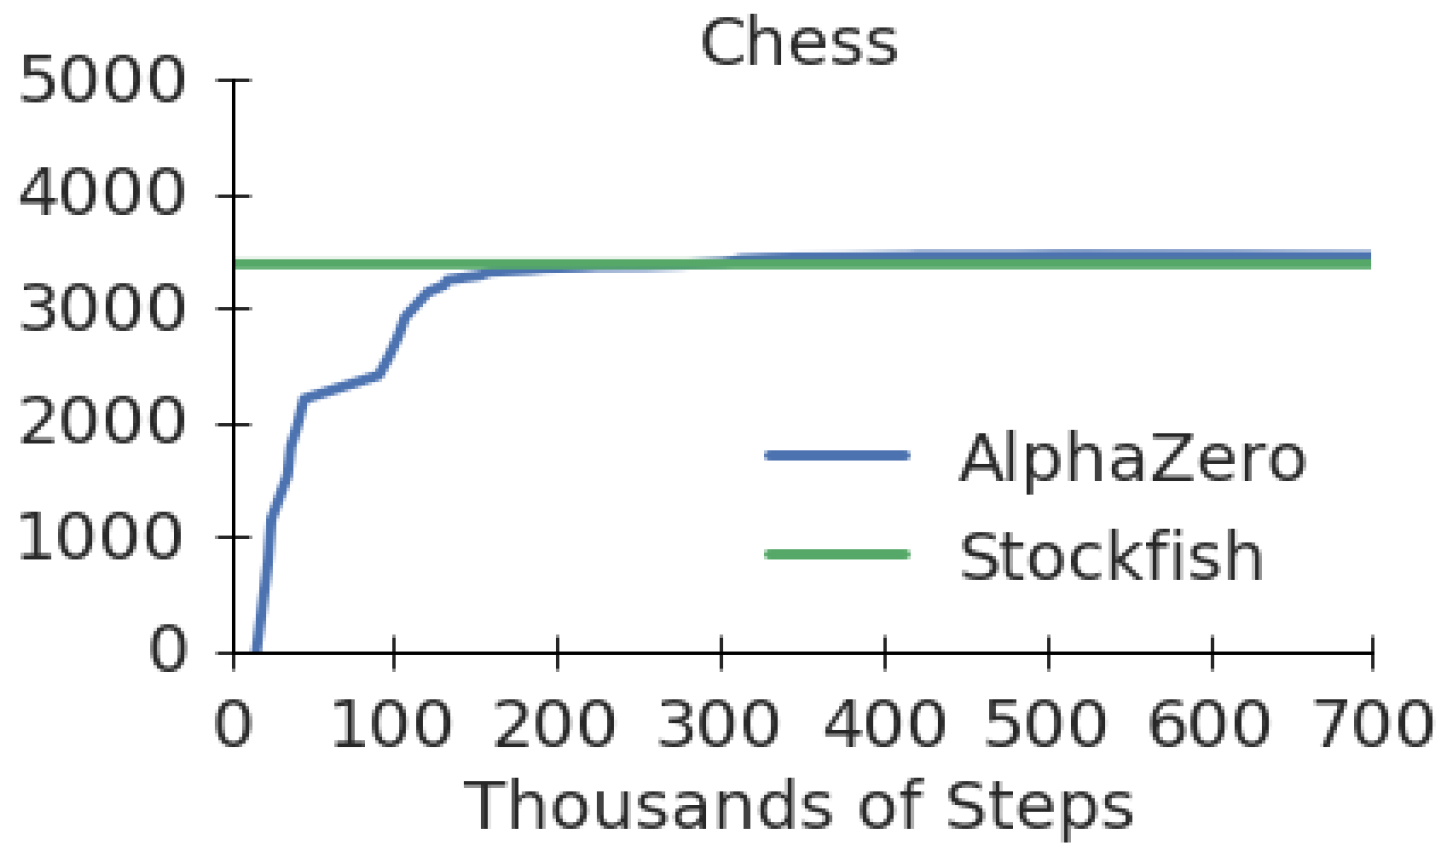
\includegraphics[width=.5\textwidth]{../img/AlphaZero-paper/elo-vs-training-chess.png}
        \pause
        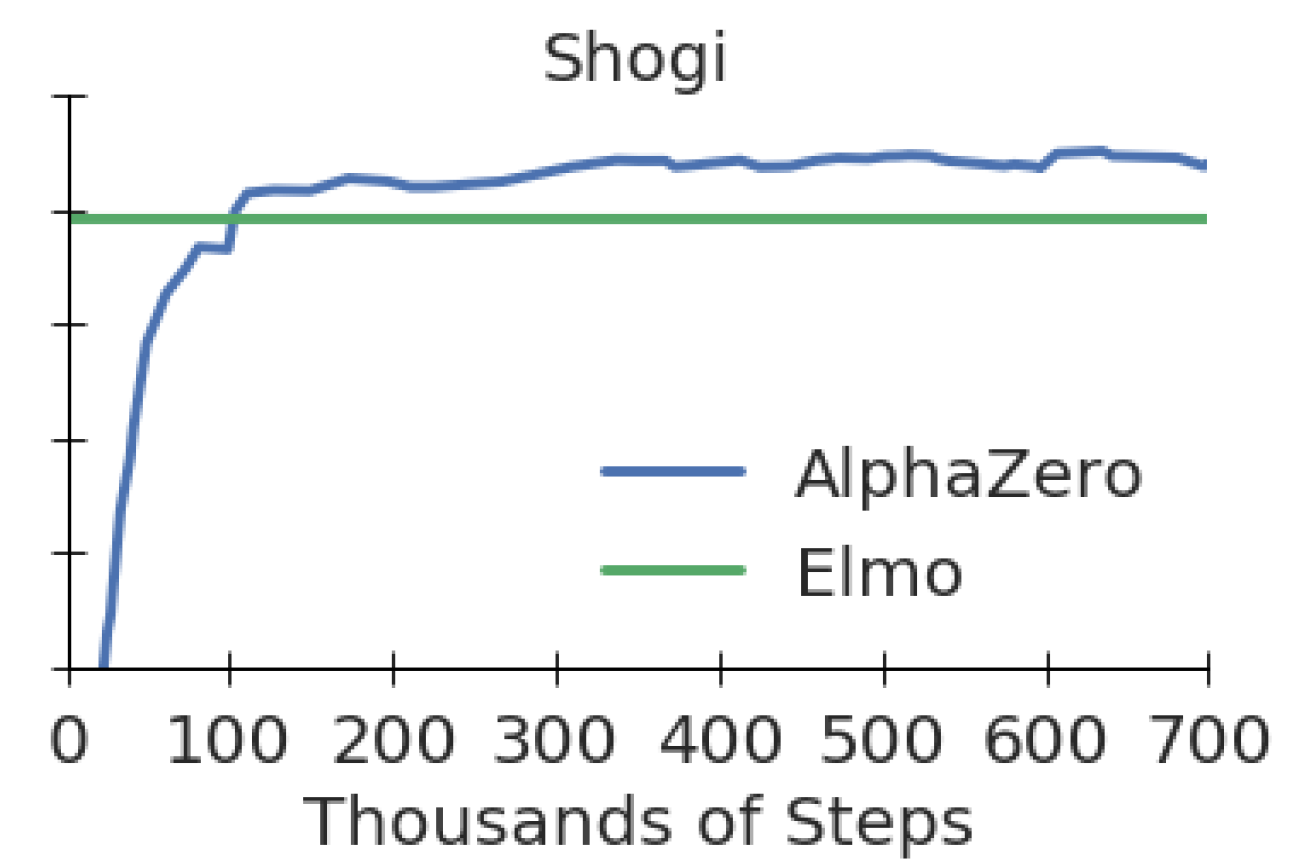
\includegraphics[width=.5\textwidth]{../img/AlphaZero-paper/elo-vs-training-shogi.png}

        \pause
        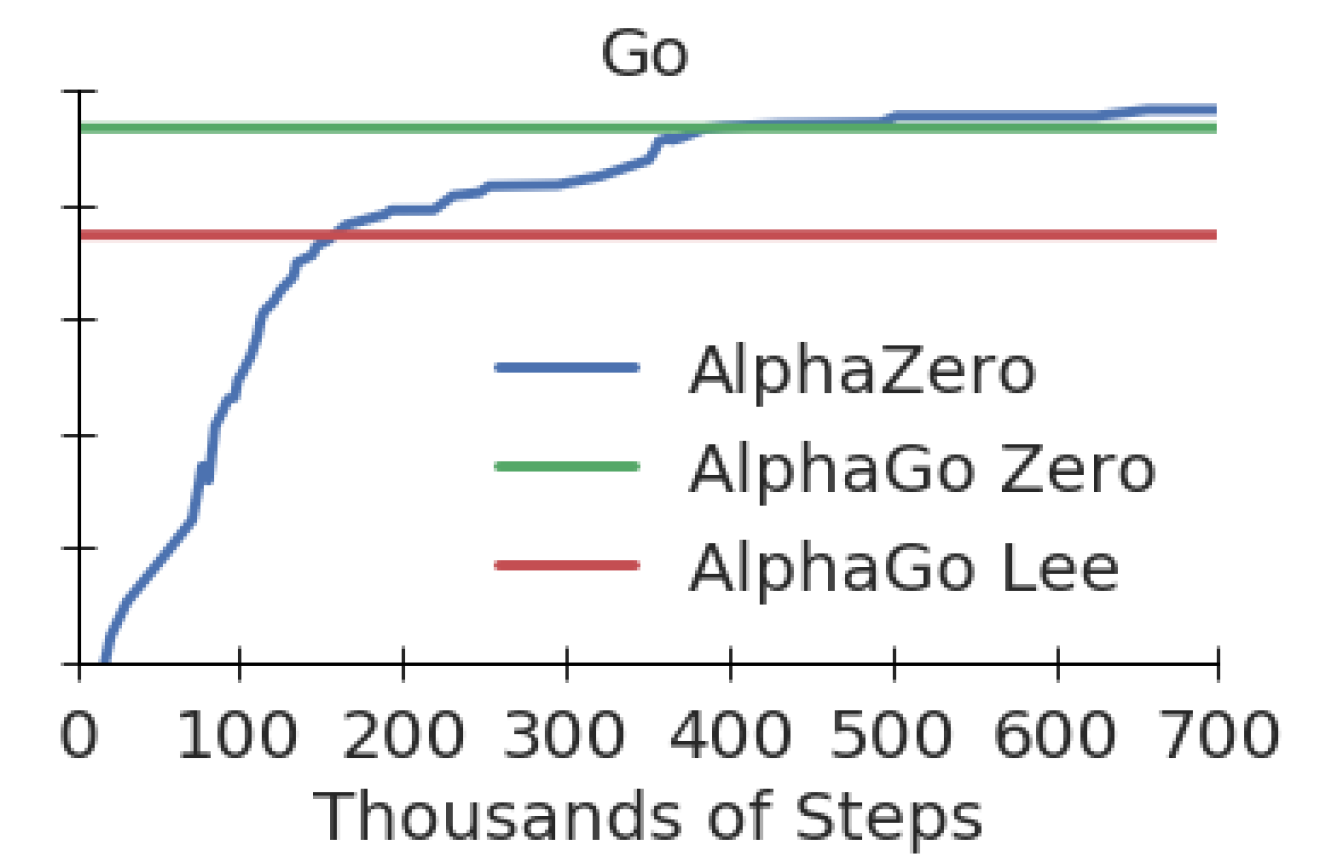
\includegraphics[height=.4\textheight]{../img/AlphaZero-paper/elo-vs-training-go.png}
      \end{center}
    \end{frame}

    \begin{frame}{AlphaZero: Tournament between AI Programs}
      \begin{center}
        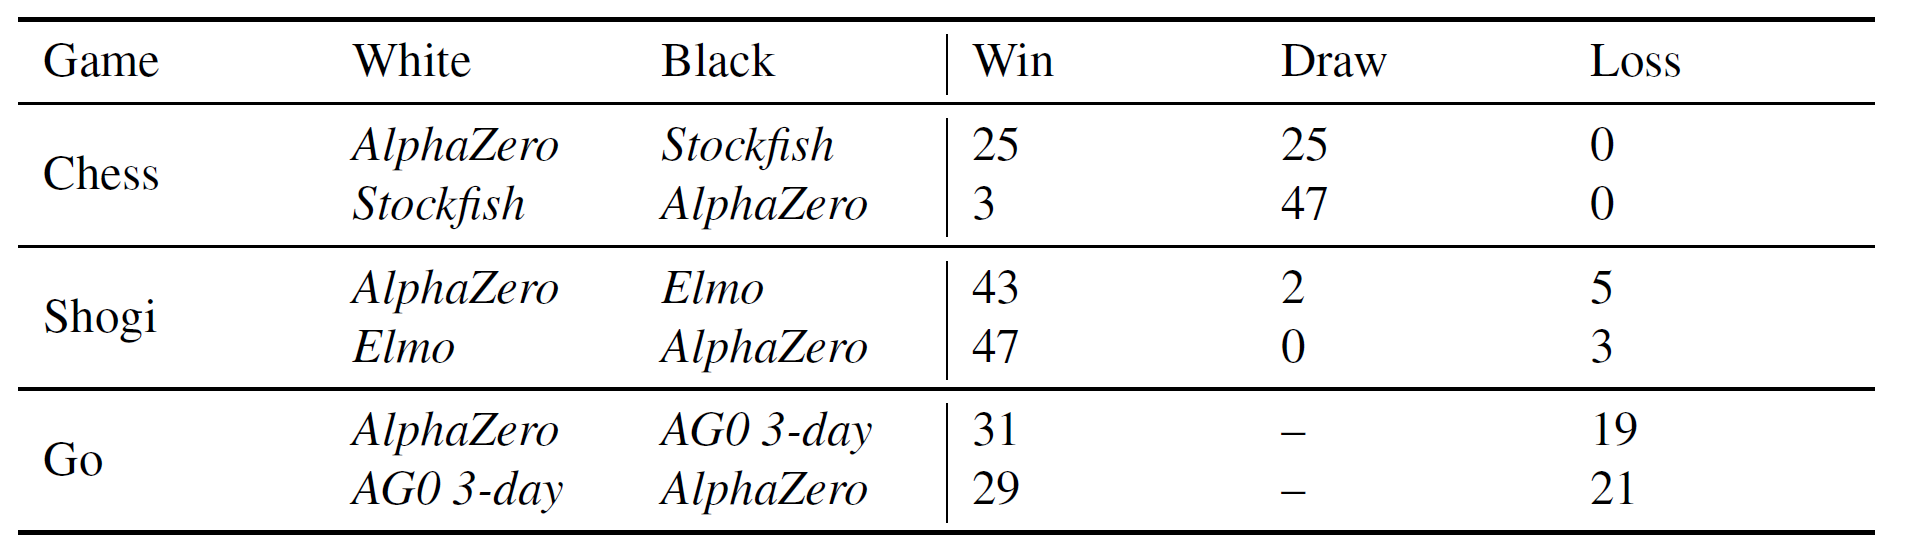
\includegraphics[width=\textwidth]{../img/AlphaZero-paper/tournament-evaluation.png}
      \end{center}

      {\tiny (Values are given from AlphaZero's point of~view.)}
    \end{frame}

    \begin{frame}{AlphaZero: Statistics of Training}
      \begin{center}
        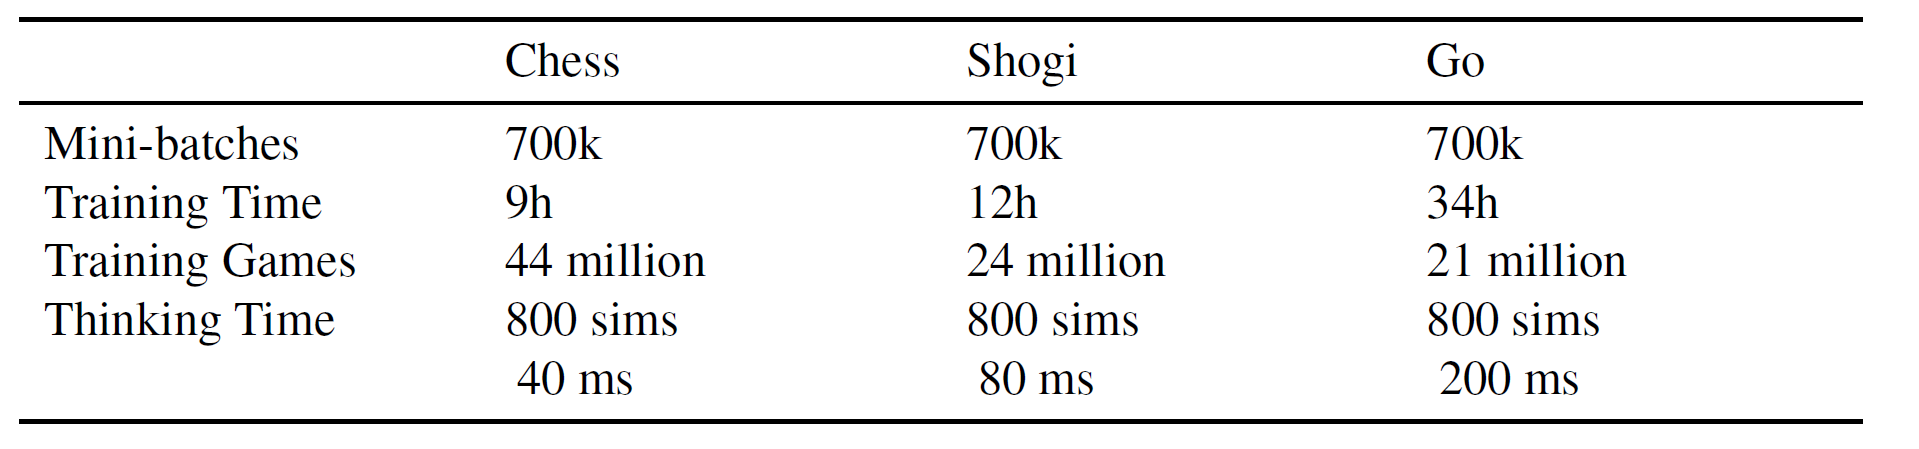
\includegraphics[width=\textwidth]{../img/AlphaZero-paper/statistics-of-AlphaZero-training.png}
      \end{center}
    \end{frame}

    \begin{frame}{AlphaZero: Evaluation Speeds}
      \begin{center}
        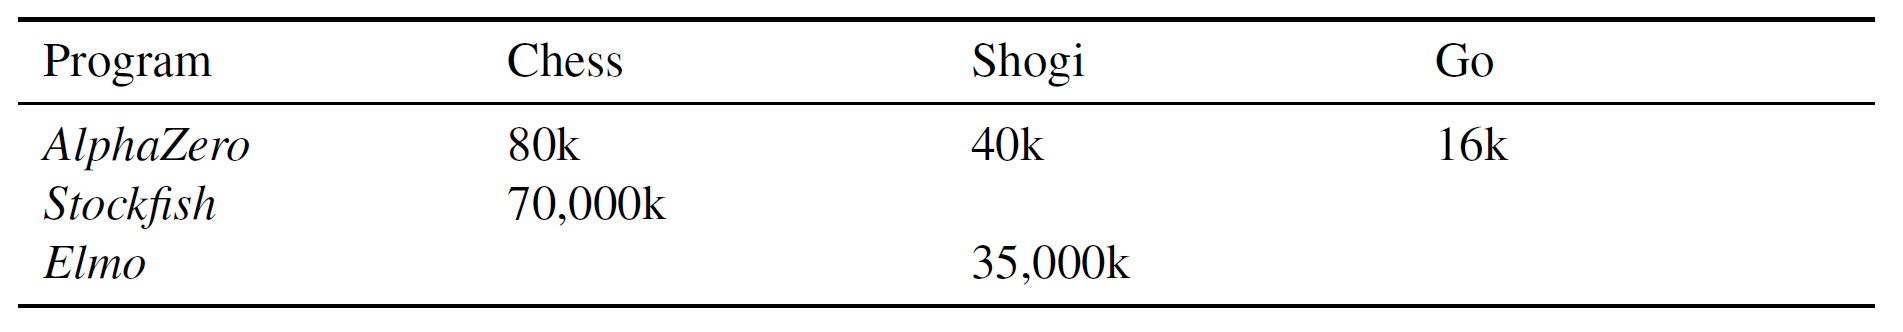
\includegraphics[width=\textwidth]{../img/AlphaZero-paper/evaluation-speed-of-AlphaZero.png}
      \end{center}
    \end{frame}
  }

  \begin{frame}[standout]
    \begin{center}
      Thank you!

      Questions?
    \end{center}
  \end{frame}

  \begin{frame}[standout]
    Backup Slides
  \end{frame}

  {
    \setbeamertemplate{frame footer}{[\cite{Silver2017AlphaZero}]}

    \begin{frame}{Input Features of AlphaZero's Neural Networks}
      \begin{center}
        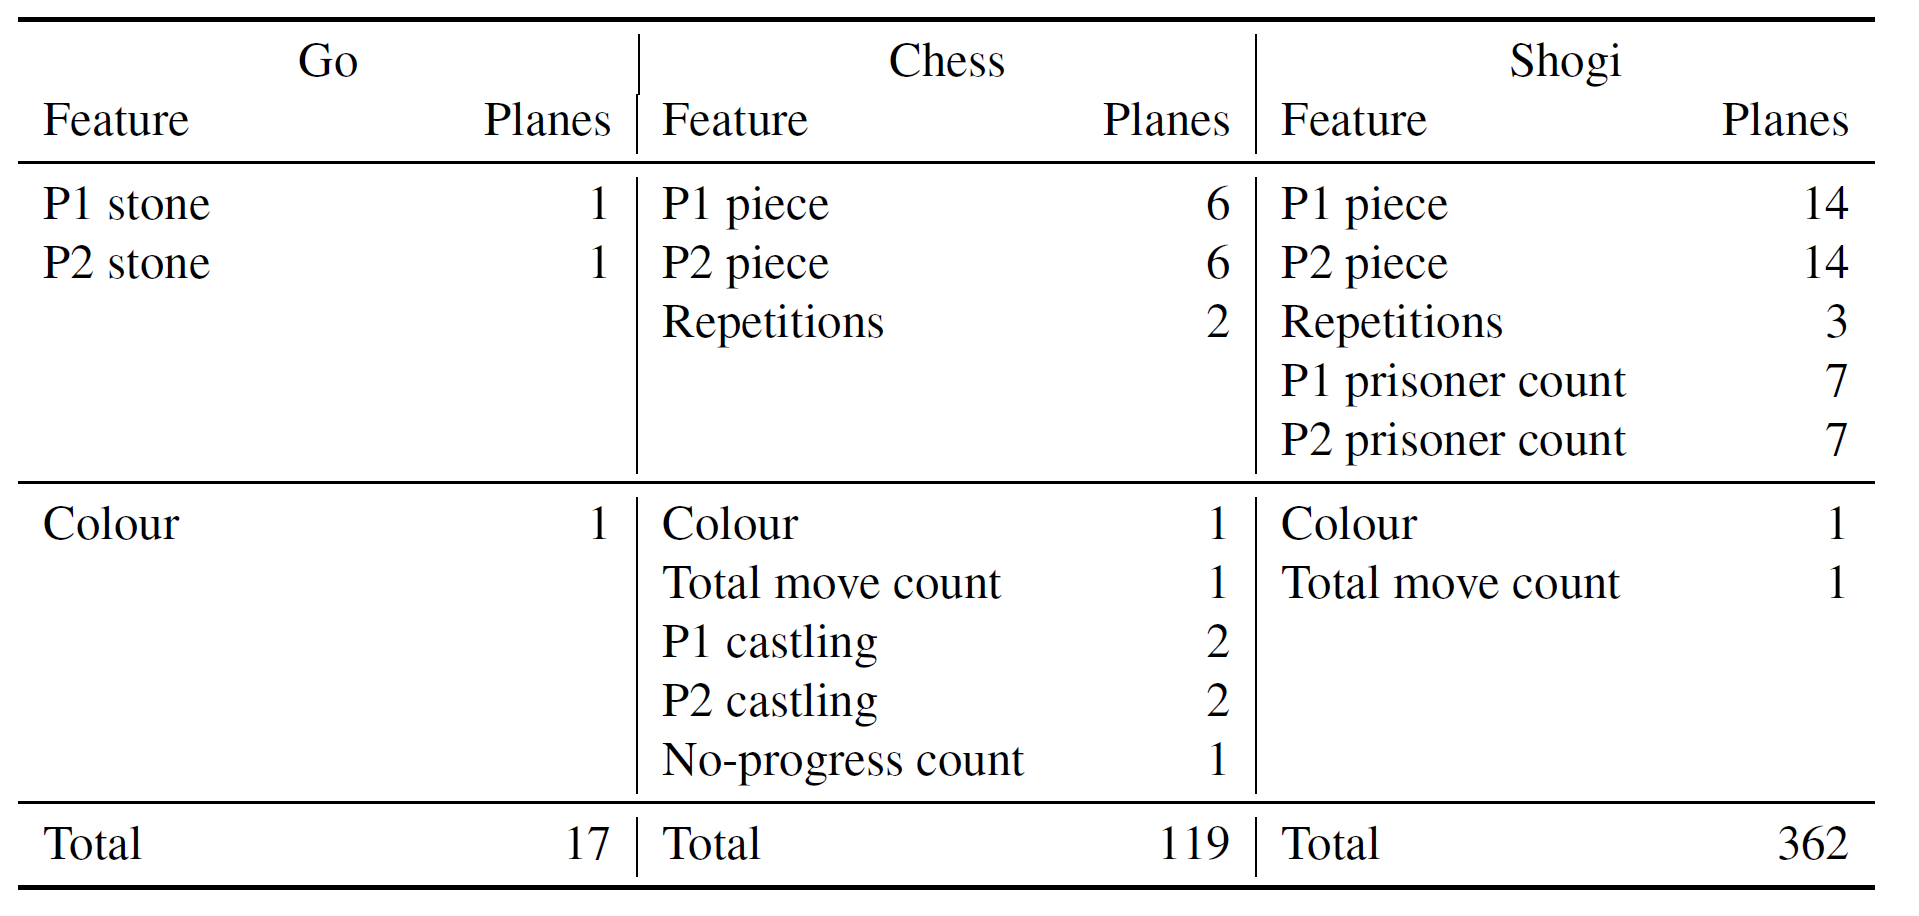
\includegraphics[width=\textwidth]{../img/AlphaZero-paper/input-features.png}
      \end{center}
    \end{frame}

    \begin{frame}{Scalability When Compared to Other Programs}
      \begin{center}
        \pause
        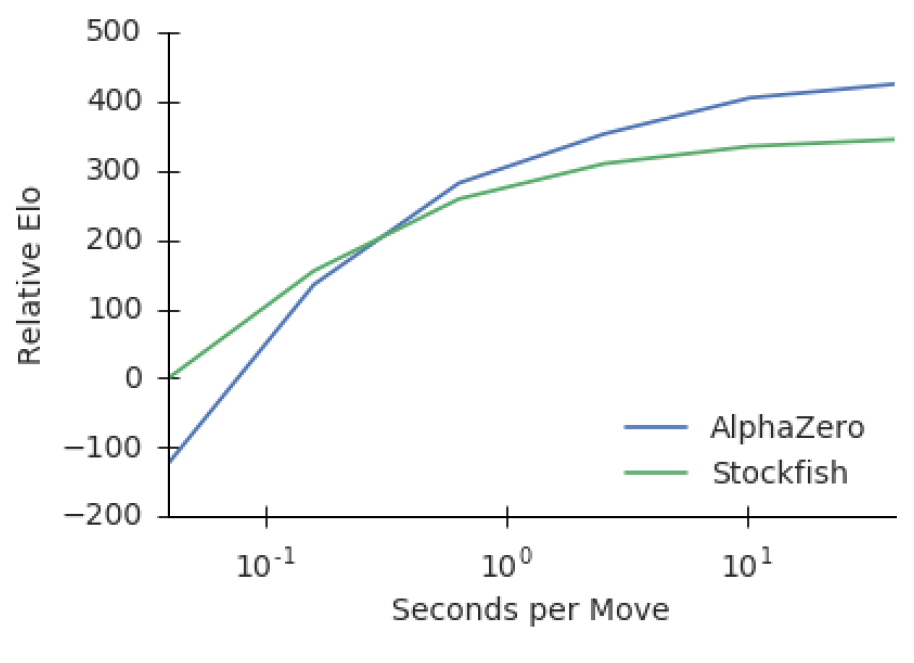
\includegraphics[height=.45\textheight]{../img/AlphaZero-paper/scalability-against-stockfish.png}

        \pause
        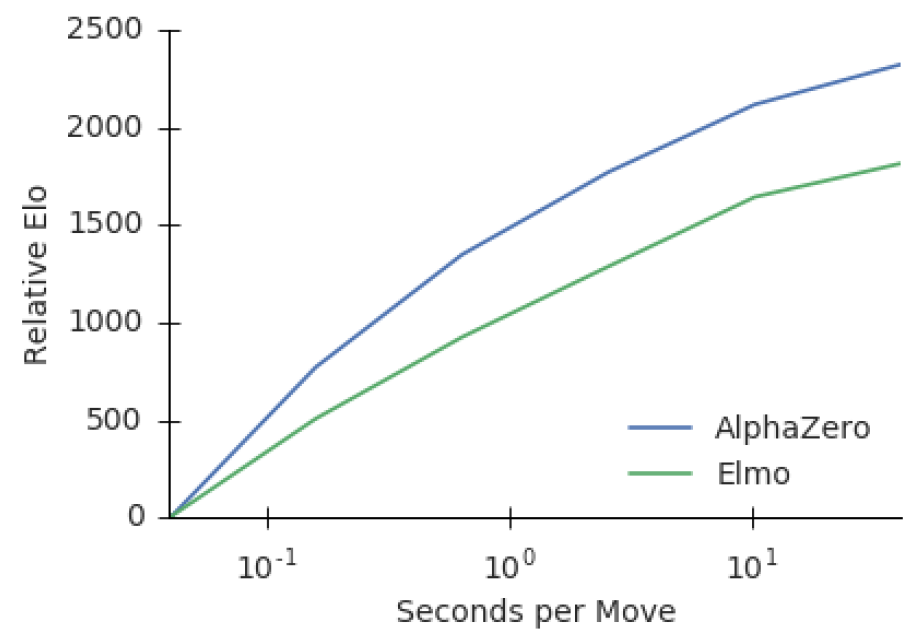
\includegraphics[height=.45\textheight]{../img/AlphaZero-paper/scalability-against-elmo.png}
      \end{center}
    \end{frame}
  }

%%%%%%%%%%%%%%%%%%%%%%%%%%%%%%%%%%%%%%%%%%%%%%%%%%%%%%%%%%%%%%%%%%%%%%%%%%%%%%%%
% LEGACY SLIDES (from AlphaGo-presentation)
%%%%%%%%%%%%%%%%%%%%%%%%%%%%%%%%%%%%%%%%%%%%%%%%%%%%%%%%%%%%%%%%%%%%%%%%%%%%%%%%

  \begin{frame}[standout]
    Legacy Slides
  \end{frame}

  \section{Why AI?}

  \begin{frame}{Applications of AI}
    \begin{itemize}[<+- | alert@+>]
      \item spam filters
      \item recommender systems (Netflix, YouTube)
      \item predictive text (Swiftkey)
      \item audio recognition (Shazam, SoundHound)
      \item self-driving cars
    \end{itemize}
  \end{frame}

  {
    \setbeamertemplate{frame footer}{[1] \cite{GatysEB15a} [2] \cite{LiW16}}
    \begin{frame}{Artistic-Style Painting (1/2)}
      \begin{center}
        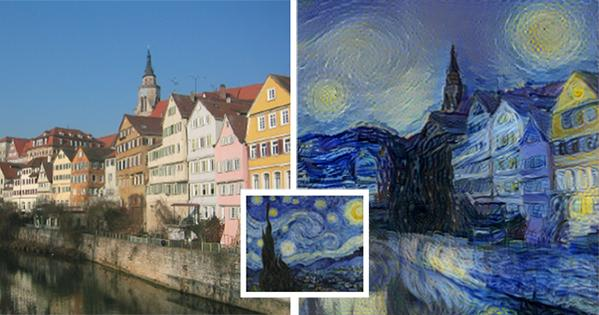
\includegraphics[height=.4\textheight]{../img/art_Van_Gogh.jpg}
        \pause

        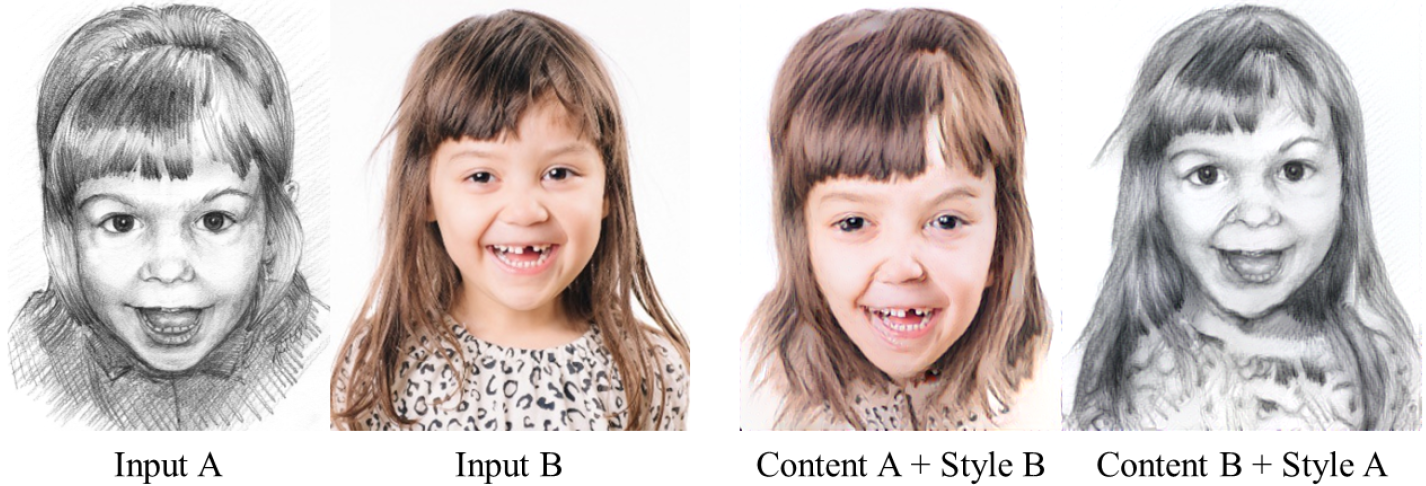
\includegraphics[height=.44\textheight]{../img/art_girl.png}
      \end{center}
    \end{frame}
  }

  {
    \setbeamertemplate{frame footer}{\cite{Champandard2016semantic}}
    \begin{frame}{Artistic-Style Painting (2/2)}
      \begin{center}
        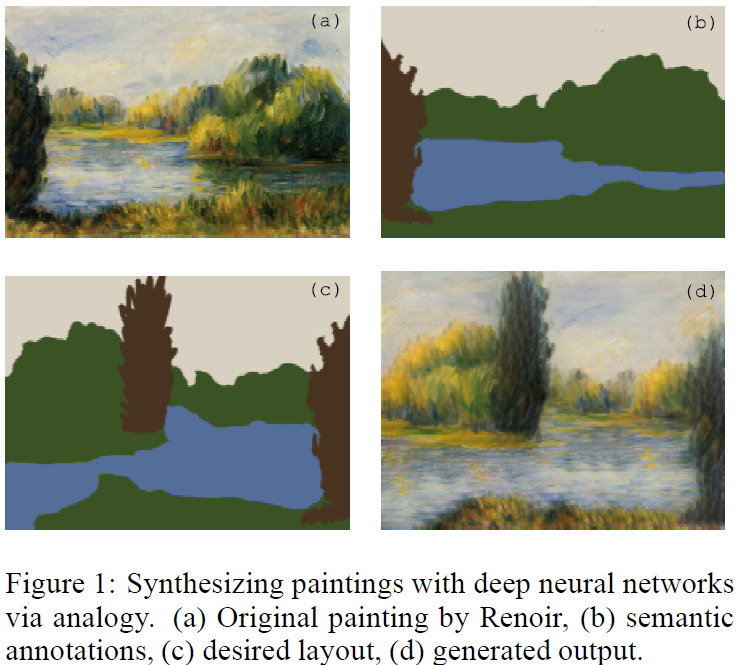
\includegraphics[height=.86\textheight,keepaspectratio]{../img/doodle_AI.png}
      \end{center}
    \end{frame}
  }

  {
    \setbeamertemplate{frame footer}{\cite{Karpathy15}}
    \begin{frame}{\alert{C Code} Generated Character by Character}
      \begin{center}
        \vskip -1.1ex
        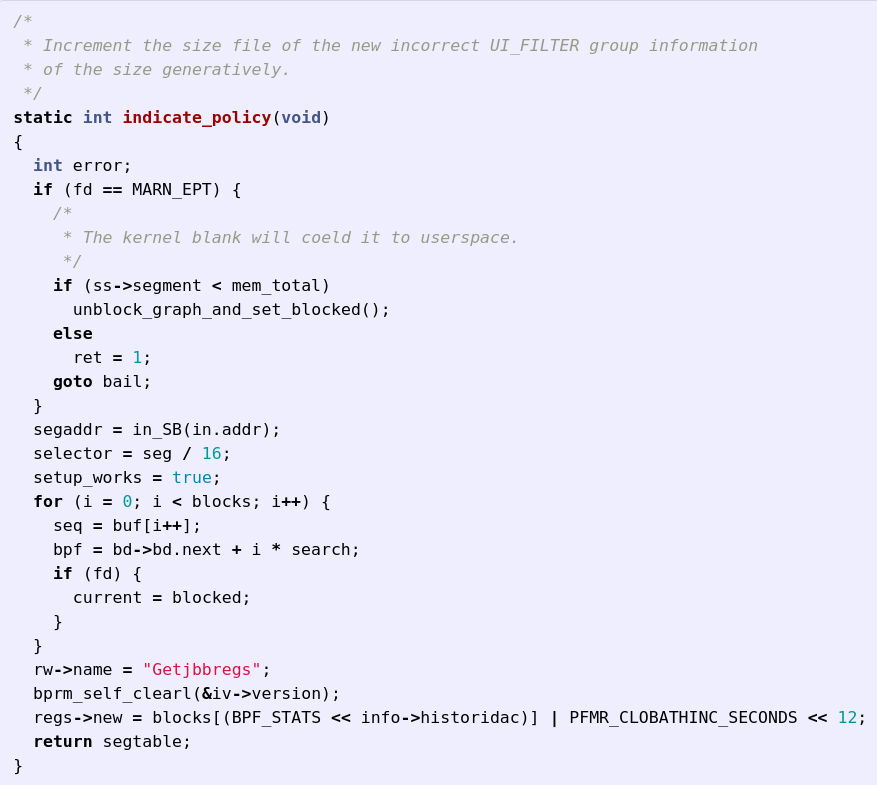
\includegraphics[height=.89\textheight, keepaspectratio]{../img/generating_c.png}
      \end{center}
    \end{frame}

    \begin{frame}{\alert{Algebraic Geometry} Generated Character by Character}
      \begin{center}
        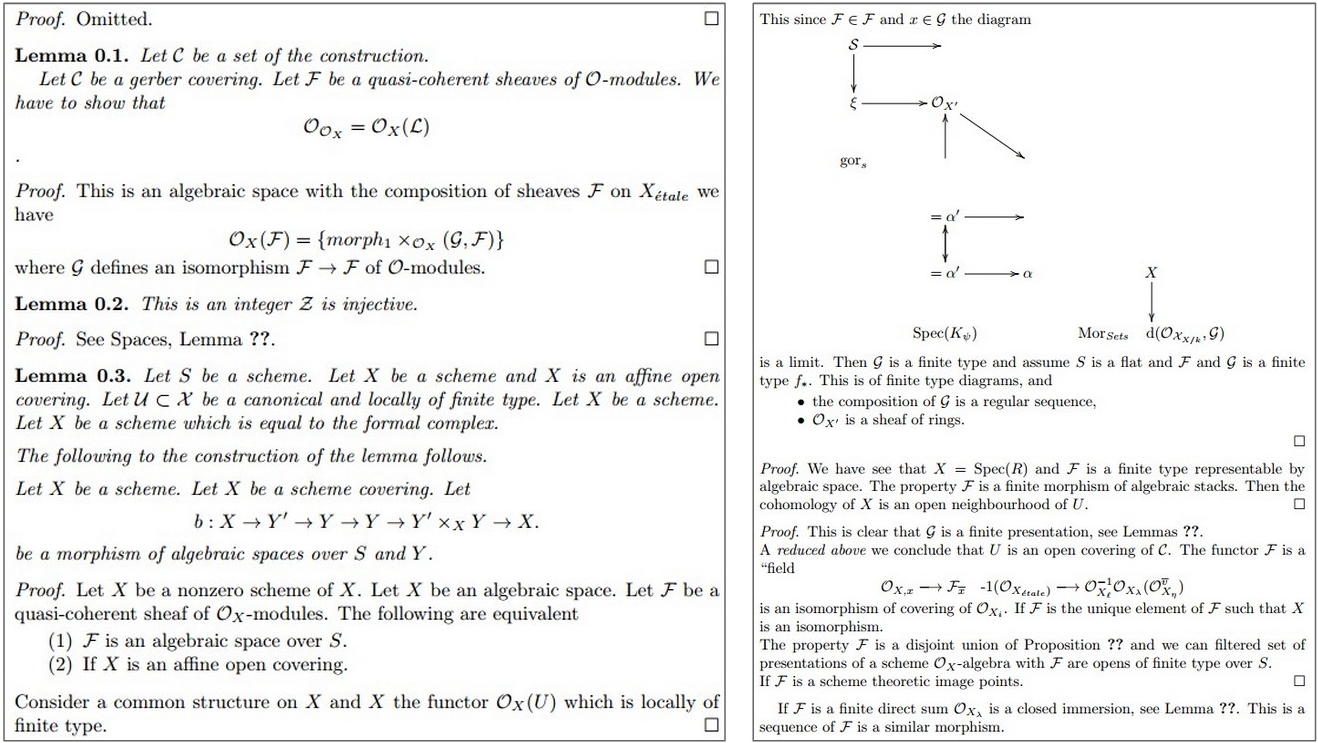
\includegraphics[width=\textwidth, height=\textheight, keepaspectratio]{../img/generating_latex.png}
      \end{center}
    \end{frame}
  }

  {
    \usebackgroundtemplate{%
      \tikz[overlay,remember picture] \node[opacity=1.0, at=(current page.center)] {
         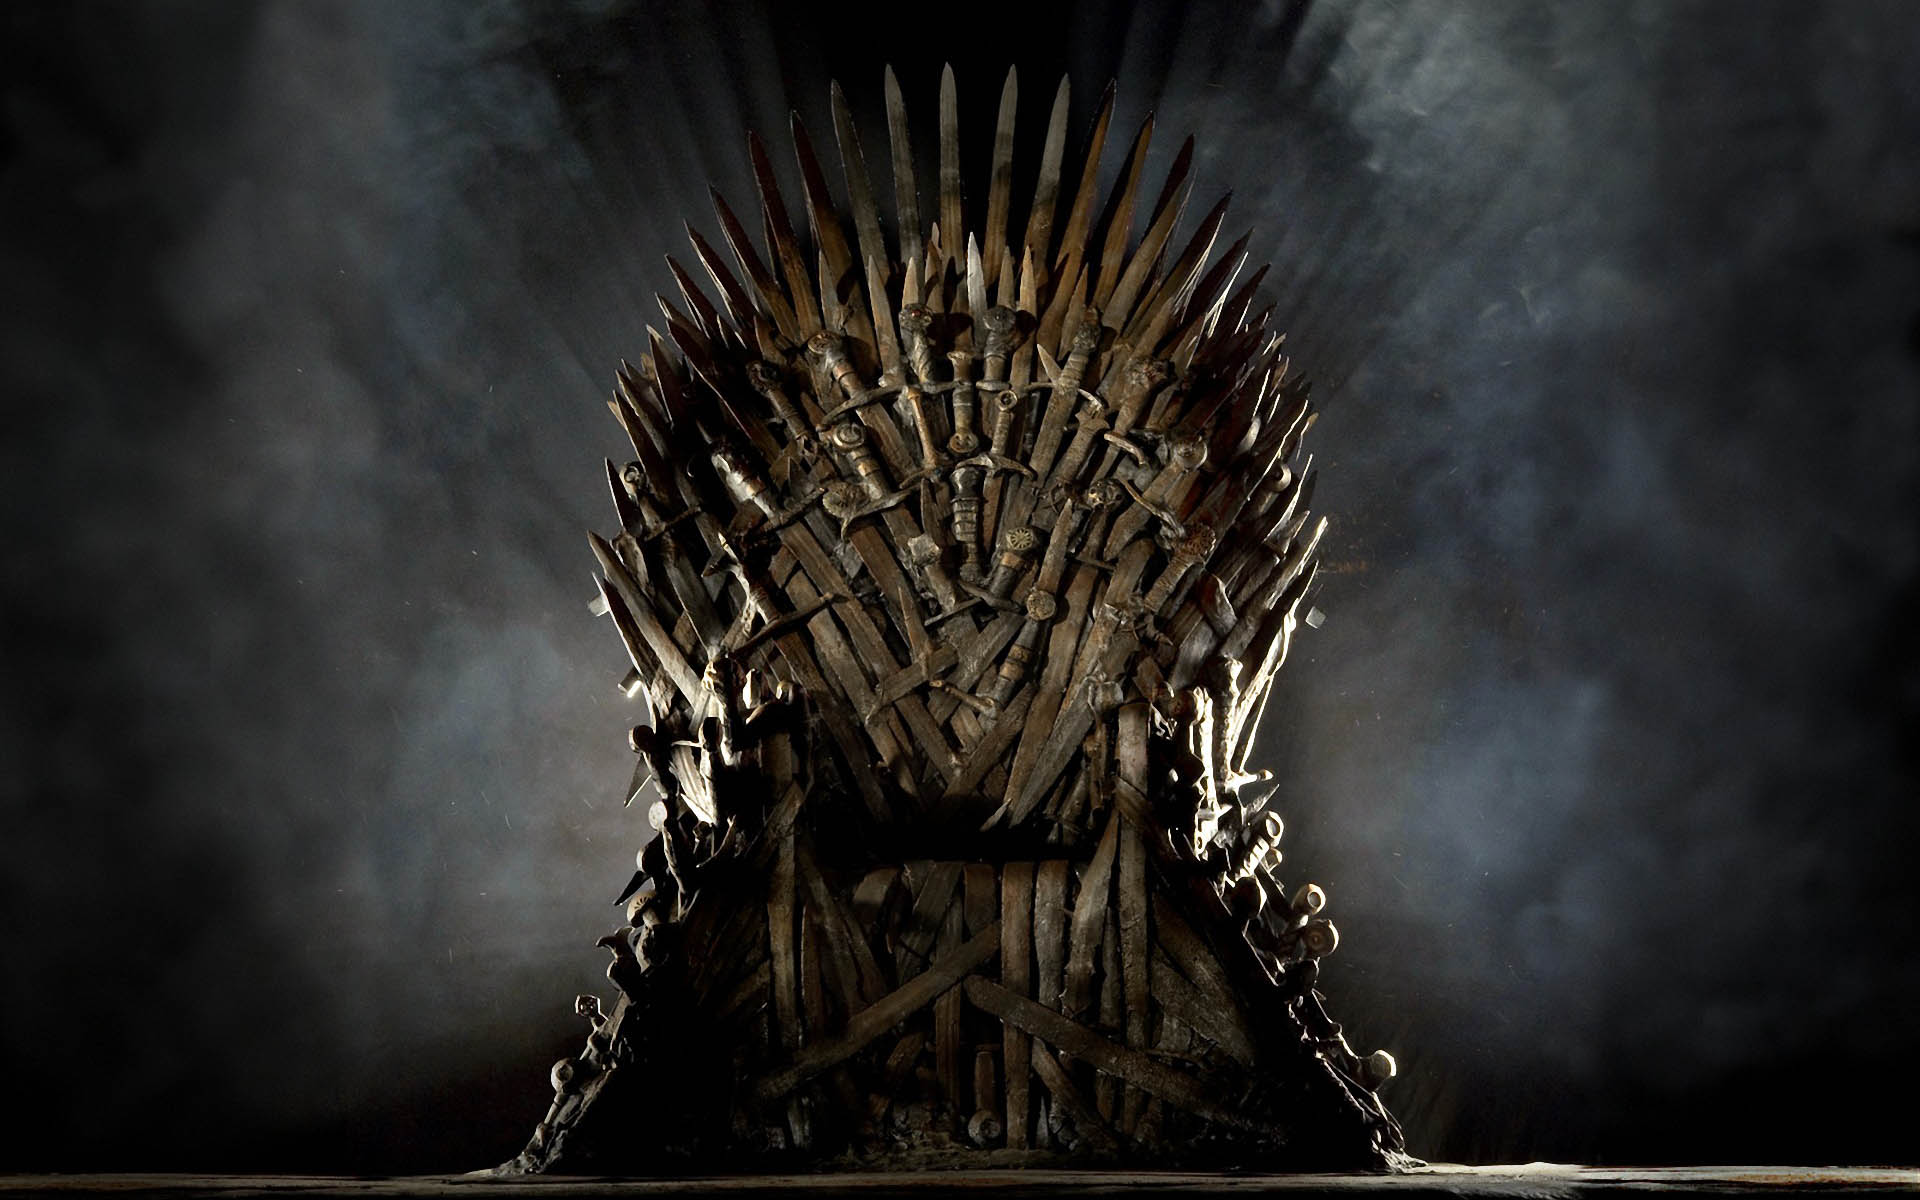
\includegraphics[height=\paperheight, keepaspectratio]{../img/Game_of_Thrones.jpg}
       };
    }
    \setbeamertemplate{frame footer}{\url{http://pjreddie.com/darknet/rnns-in-darknet/}}
    \begin{frame}[standout]
      \vskip -1em
      \tabto{-0.6cm}
      \mbox{\alert{Game of Thrones} Generated Character by Character}
      \pause

      \epigraph{
        \tiny
        JON
        \epiParSpace
        He leaned close and onions, barefoot from his shoulder.
        ``I am not a purple girl,'' he said as he stood over him.
        ``The sight of you sell your father with you a little choice.''
        \epiParSpace
        ``I say to swear up his sea or a boy of stone and heart, down,'' Lord Tywin said.
        ``I love your word or her to me.''
      }{Darknet (on Linux)}
      \pause
      \vskip -1.5em
      \epigraph{
        \tiny
        JON
        \epiParSpace
        Each in days and the woods followed his king.
        ``I understand.''
        \epiParSpace
        ``I am not your sister Lord Robert?''
        \epiParSpace
        ``The door was always some cellar to do his being girls and the Magnar of Baratheon, and there were thousands of every bite of half the same as though he was not a great knight should be seen, and not to look at the Redwyne two thousand men.''
      }{Darknet (on OS X)}
    \end{frame}
  }

  {
    \setbeamertemplate{frame footer}{\cite{DeepDrumpf}}
    \usebackgroundtemplate{
      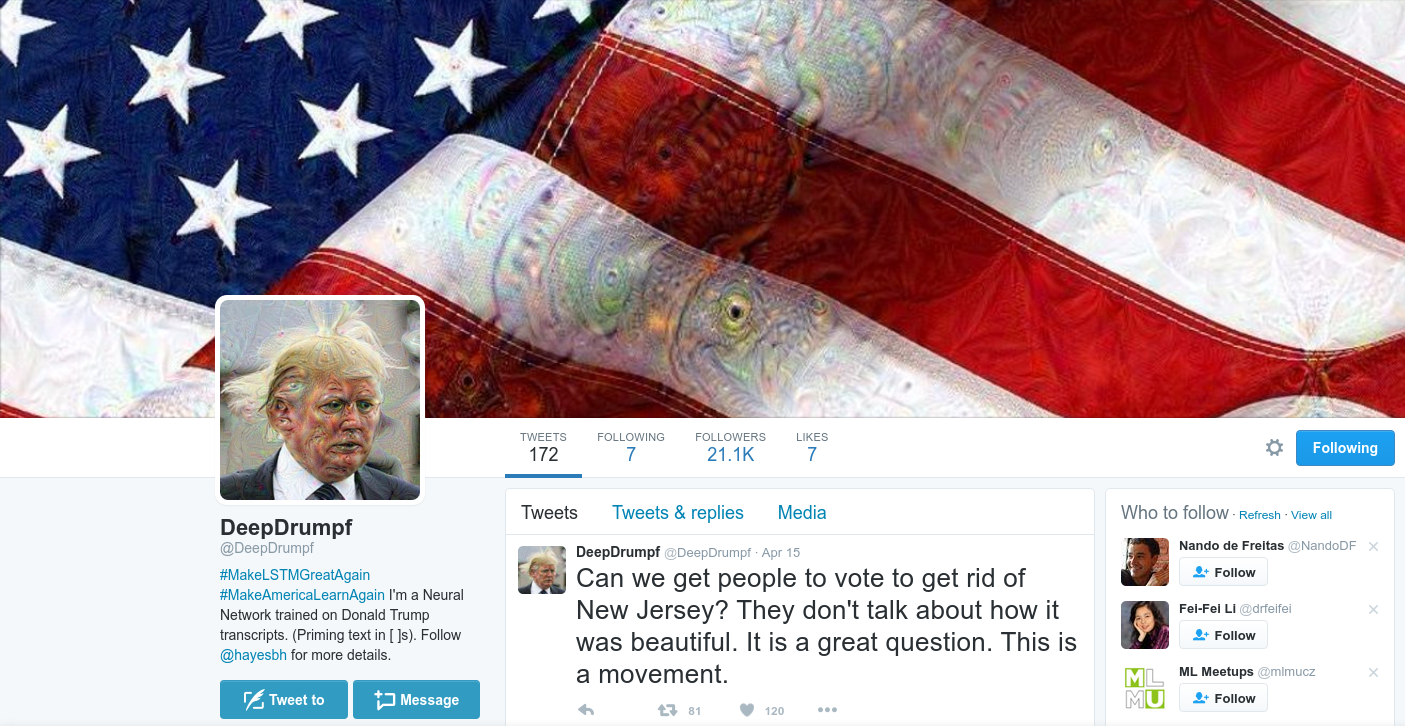
\includegraphics[height=\paperheight, width=\paperwidth, keepaspectratio]{../img/DeepDrumpf_zoomed_in.png}
    }

    \begin{frame}{DeepDrumpf: a~Twitter bot / neural network which learned the~language of Donald Trump from his speeches}
      \pause

      \vskip 5.25cm
      \begin{itemize}[<+- | alert@+>]
          \tiny
        \item We've got nuclear weapons that are obsolete.
          I'm going to create jobs just by making the worst thing ever.
        \item The biggest risk to the world, is me, believe it or not.
        \item I am what ISIS doesn't need.
        \item I'd like to beat that \href{https://twitter.com/hillaryclinton}{@HillaryClinton}.
          She is a horror.
          I told my supporter Putin to say that all the time.
          He has been amazing.
        \item I buy Hillary, it's beautiful and I'm happy about it.
      \end{itemize}
    \end{frame}
  }

  {
    \setbeamertemplate{frame footer}{\cite{Mnih2015human}}
    \begin{frame}{Atari Player by Google DeepMind}
      \begin{center}
        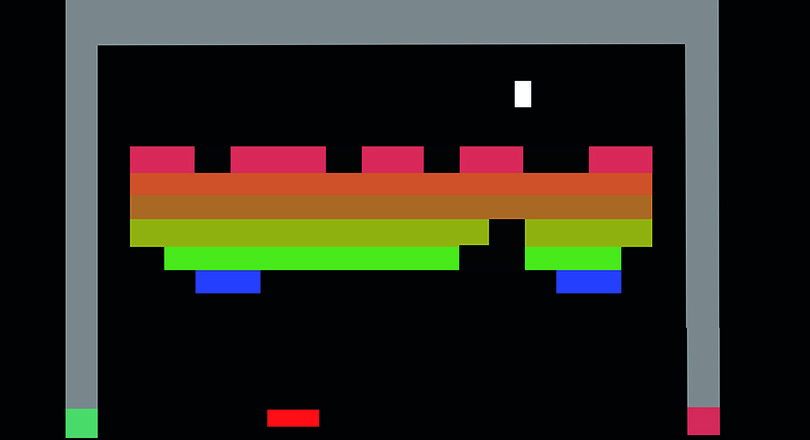
\includegraphics[width=\textwidth, height=\textheight, keepaspectratio]{../img/atari_breakout.jpg}

        \url{https://youtu.be/0X-NdPtFKq0?t=21m13s}
      \end{center}
    \end{frame}
  }

  {
    \setbeamertemplate{frame footer}{\color{gray}\url{https://xkcd.com/1002/}}
    \begin{frame}[standout]
      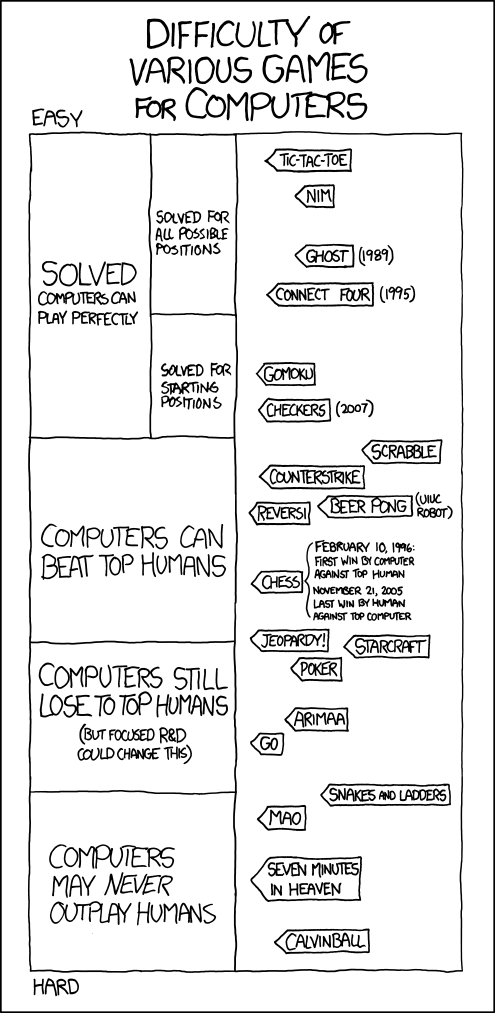
\includegraphics[height=\paperheight]{../img/game_AIs.png}
    \end{frame}
  }

  {
    \setbeamertemplate{frame footer}{\cite{Bowling2015heads}}
    \begin{frame}{Heads-up Limit Hold’em Poker Is Solved!}
      \begin{center}
        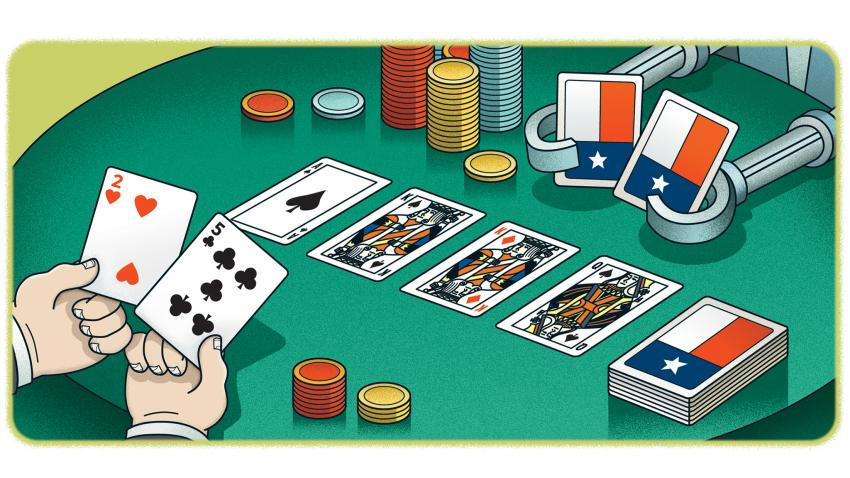
\includegraphics[width=\textwidth, keepaspectratio]{../img/limit_holdem_poker.jpg}
        \pause

        \textbf{Cepheus} \url{http://poker.srv.ualberta.ca/} \\
        {\tiny 0.000986 big blinds per game on expectation}
      \end{center}
    \end{frame}
  }

%%%%%%%%%%%%%%%%%%%%%%%%%%%%%%%%%%%%%%%%%%%%%%%%%%%%%%%%%%%%%%%%%%%%%%%%%%%%%%%%

  \section{Basics of Machine Learning}

  {
    \setbeamertemplate{frame footer}{\color{gray} \url{https://dataaspirant.com/2014/09/19/supervised-and-unsupervised-learning/}}
    \begin{frame}[standout]
      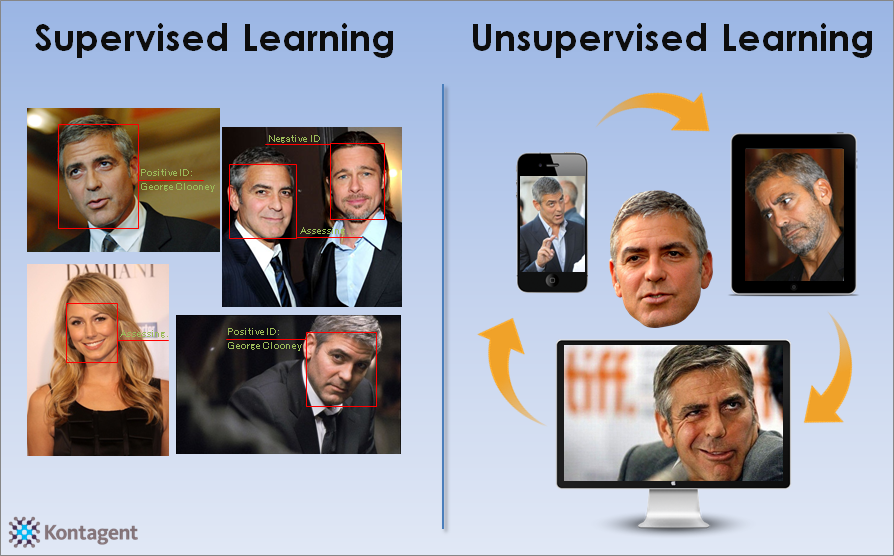
\includegraphics[width=\textwidth]{../img/SL_vs_UL_George_Clooney.png}
    \end{frame}
  }

  {
    \setbeamertemplate{frame footer}{\url{http://www.nickgillian.com/}}
    \begin{frame}{Supervised Learning (SL)}
      \begin{center}
        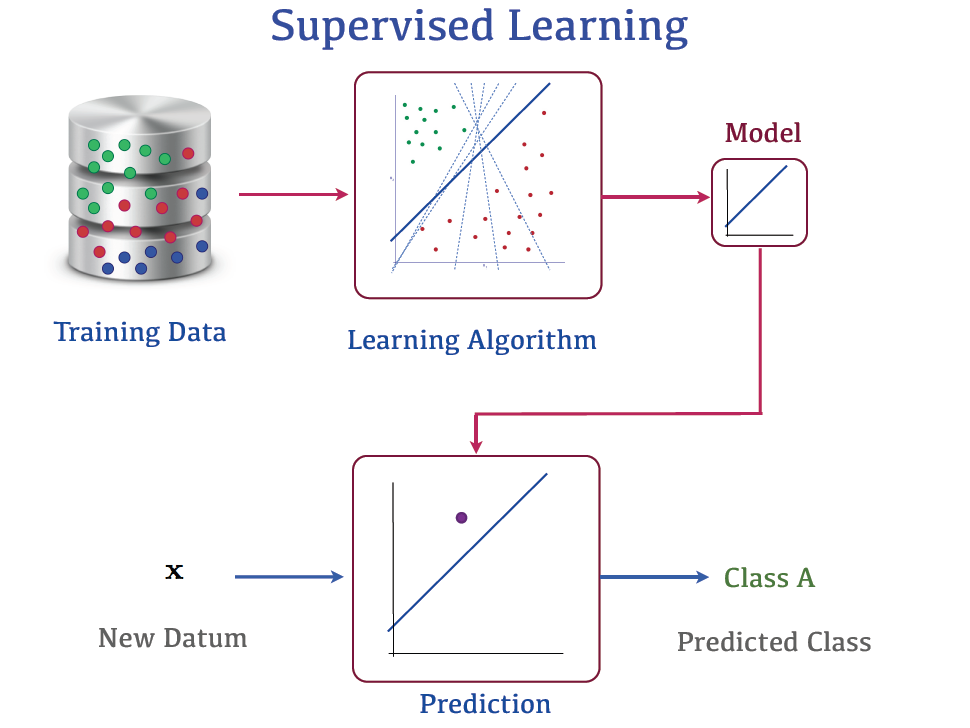
\includegraphics[height=.6\textheight]{../img/SL_workflow.png}
      \end{center}
      \pause

      \begin{enumerate}[<+- | alert@+>]
          \tiny
        \item data collection: Google Search, Facebook ``Likes'', Siri, Netflix, YouTube views, LHC collisions, \textbf{KGS Go Server}...
        \item training on~\textbf{training set}
        \item testing on~\textbf{testing set}
        \item deployment
      \end{enumerate}
      \pause
    \end{frame}
  }

  \begin{frame}[standout]{Regression}
    \pause
    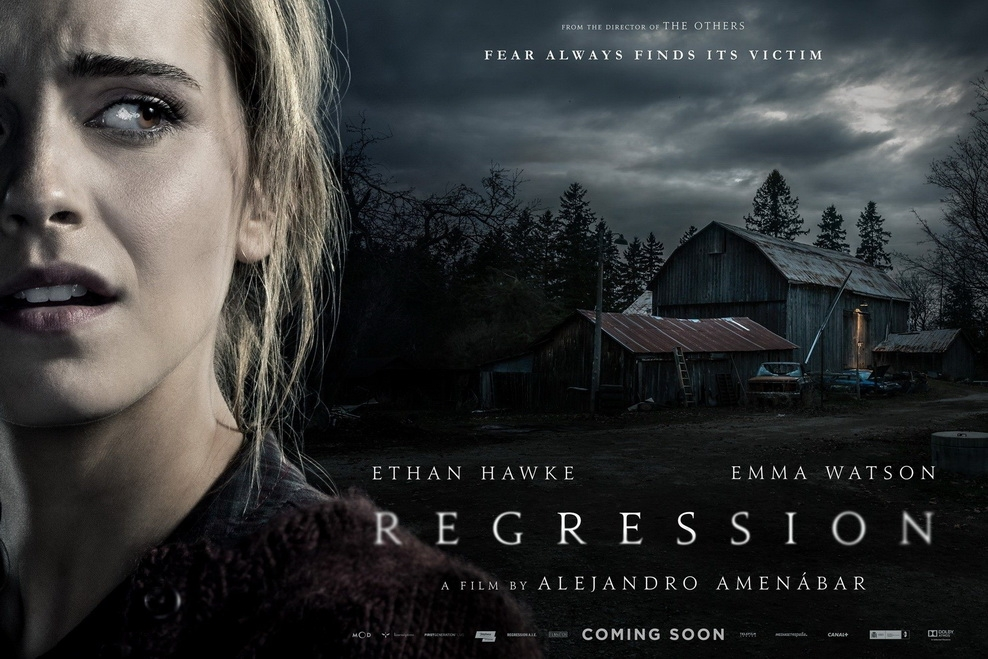
\includegraphics[width=\textwidth]{../img/regression_movie.jpg}
  \end{frame}

  {
    \setbeamertemplate{frame footer}{\url{https://thermanuals.wordpress.com/descriptive-analysis/sampling-and-regression/}}
    \begin{frame}{Mathematical Regression}
      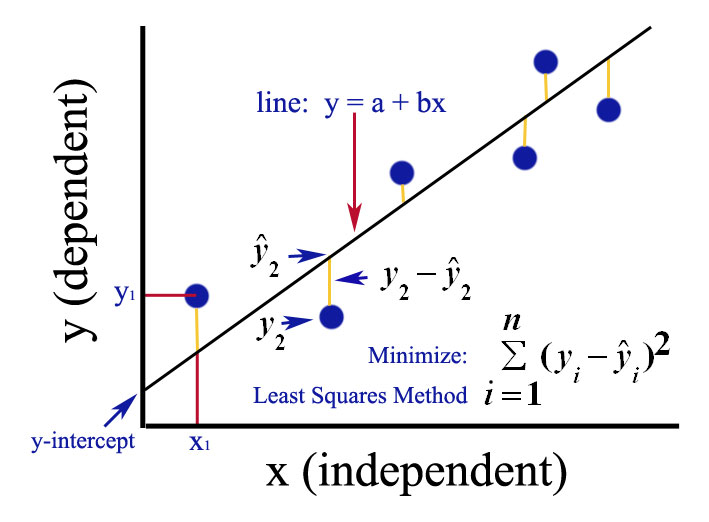
\includegraphics[width=\textwidth]{../img/regression_math.jpg}
    \end{frame}
  }

  {
    \setbeamertemplate{frame footer}{\url{https://kevinbinz.files.wordpress.com/2014/08/ml-svm-after-comparison.png}}
    \begin{frame}{Classification}
      \includegraphics[width=\textwidth]{../img/classification.png}
    \end{frame}
  }

  {
    \setbeamertemplate{frame footer}{\url{https://www.researchgate.net/post/How_to_Avoid_Overfitting}}
    \begin{frame}{Underfitting and Overfitting}
      \begin{center}
        \includegraphics[width=.75\textwidth]{../img/underfitting_and_overfitting.jpg}
        \pause
      \end{center}

      Beware of~overfitting!
      \pause

      It is like learning for~a~mathematical exam by~memorizing proofs.
    \end{frame}
  }

  {
    \setbeamertemplate{frame footer}{\url{https://youtu.be/0X-NdPtFKq0?t=16m57s}}
    \setbeamercolor{background canvas}{bg=gray!12}
    \begin{frame}{Reinforcement Learning (RL)}
      \begin{center}
        \includegraphics[width=\textwidth]{../img/RL_framework.png}
      \end{center}
      \pause
      
      Specially: games of \textbf{self-play}
    \end{frame}
  }

%%%%%%%%%%%%%%%%%%%%%%%%%%%%%%%%%%%%%%%%%%%%%%%%%%%%%%%%%%%%%%%%%%%%%%%%%%%%%%%%

  \section{Monte Carlo Tree Search}
  {
    \setbeamertemplate{frame footer}{\cite{Silver2016mastering}}
    \begin{frame}{Tree Search}
      Optimal value~$v^*(s)$ determines the~outcome of~the game:
      \pause
      \begin{itemize}[<+- | alert@+>]
          \tiny
        \item from every board position or state $s$
        \item under perfect play by~all players.
      \end{itemize}
      \pause

      It is computed by~\textbf{recursively traversing a~search tree} containing approximately $b^d$ possible sequences of moves, where
      \pause
      \begin{itemize}[<+- | alert@+>]
          \tiny
        \item $b$ is the game’s breadth (number of legal moves per position)
        \item $d$ is its depth (game length)
      \end{itemize}
    \end{frame}
  }

  {
    \setbeamertemplate{frame footer}{\cite{Allis1994searching}}
    \begin{frame}{Game tree of~Go}
      Sizes of~trees for~various games:
      \begin{itemize}
        \item chess: $b \approx 35, d \approx 80$
        \item Go: $b \approx 250, d \approx 150$
          \pause
          $\Rightarrow$ more positions than atoms in the universe!
      \end{itemize}
      \pause

      \epigraph{
        That makes Go a \textbf{googol} [$10^{100}$] times more complex than chess.
      }{\tiny\url{https://deepmind.com/alpha-go.html}}
      \pause

      \vskip -2em
      How to handle the size~of the game tree?
      \pause
      \begin{itemize}[<+- | alert@+>]
        \item for the breadth: a~neural network to~select moves 
        \item for the depth: a~neural network to~evaluate the current position
        \item for the tree traverse: Monte Carlo tree search (MCTS)
      \end{itemize}
    \end{frame}
  }

  \begin{frame}{Monte Carlo tree search}
    \includegraphics[width=\textwidth]{../img/MCTS.png}
  \end{frame}

%%%%%%%%%%%%%%%%%%%%%%%%%%%%%%%%%%%%%%%%%%%%%%%%%%%%%%%%%%%%%%%%%%%%%%%%%%%%%%%%

  \section{Neural networks}
  {
    \setbeamertemplate{frame footer}{\url{http://pages.cs.wisc.edu/~bolo/shipyard/neural/local.html}}
    \begin{frame}{Neural Networks (NN): Inspiration}
      \vskip -2em
      \begin{center}
        \includegraphics[height=.5\textheight]{../img/colored_neural_network.png}
      \end{center}

      \pause
      \begin{itemize}[<+- | alert@+>]
        \item inspired by~the neuronal structure of~the mammalian cerebral cortex
        \item but on~much smaller scales
        \item suitable to model systems with a~high tolerance to~error 
          \begin{itemize}
            \item e.g.~audio or~image recognition
          \end{itemize}
      \end{itemize}
    \end{frame}
  }

  {
    \setbeamertemplate{frame footer}{\cite{Dieterle2003multianalyte}}
    \begin{frame}{Neural Networks: Modes}
      \begin{center}
        \includegraphics[height=.6\textheight]{../img/neural_network_forward_and_backprop.png}
      \end{center}

      \pause
      Two modes
      \pause
      \begin{itemize}[<+- | alert@+>]
        \item \textbf{feedforward} for making predictions
        \item \textbf{backpropagation} for learning
      \end{itemize}
    \end{frame}
  }

  {
    \setbeamercolor{background canvas}{bg=gray!10}
    \setbeamertemplate{frame footer}{\url{http://stevenmiller888.github.io/mind-how-to-build-a-neural-network/}}
    \begin{frame}{Neural Networks: an~Example of~Feedforward}
      \begin{center}
        \includegraphics[width=\textwidth]{../img/feed_forward_example.png}
      \end{center}
    \end{frame}
  }

  {
    \setbeamertemplate{frame footer}{\url{http://pages.cs.wisc.edu/~bolo/shipyard/neural/local.html}}
    \begin{frame}{Gradient Descent in~Neural Networks}
      \pause
      Motto: "Learn by mistakes!"
      \begin{center}
        \includegraphics[height=.7\textheight]{../img/optimization_for_neural_networks.png}
      \end{center}
      \pause

      \vskip -1em
      However, error functions are not necessarily convex or~so ``smooth''.
    \end{frame}
  }

  {
    \setbeamertemplate{frame footer}{\color{gray}\url{http://xkcd.com/1425/}}
    \begin{frame}[standout]
      \includegraphics[height=\paperheight]{../img/tasks_bird_detection.png}
    \end{frame}
  }

  {
    \setbeamertemplate{frame footer}{\url{http://code.flickr.net/2014/10/20/introducing-flickr-park-or-bird/}}
    \begin{frame}{Convolutional Neural Networks (CNN or ConvNet)}
      \includegraphics[width=\linewidth,height=\textheight,keepaspectratio]{../img/CNN_bird_detection.png}
    \end{frame}
  }

  {
    \setbeamertemplate{frame footer}{\url{http://pages.cs.wisc.edu/~bolo/shipyard/neural/local.html}}
    \begin{frame}{(Deep) Convolutional Neural Networks}
      \begin{center}
        \tiny
        The hierarchy of~concepts is captured in~the~number of~layers: the~\textbf{deep} in~``\textbf{Deep} Learning''.
        \pause

        \includegraphics[width=\textwidth]{../img/ConvNet_hierarchy.png}
      \end{center}
    \end{frame}
  }

%%%%%%%%%%%%%%%%%%%%%%%%%%%%%%%%%%%%%%%%%%%%%%%%%%%%%%%%%%%%%%%%%%%%%%%%%%%%%%%%

  \section{Rules of Go}
  {
    \begin{frame}[standout]
      \begin{center}
        Backgammon: Man vs. Fate

        \includegraphics[height=.4\textheight]{../img/backgammon.jpg}
        \pause

        Chess: Man vs. Man

        \includegraphics[height=.4\textheight]{../img/chess.jpg}
      \end{center}
    \end{frame}
  }

  {
    \setbeamertemplate{frame footer}{\color{gray} Robert \v{S}\'{a}mal (White) versus Karel Kr\'{a}l (Black), Spring School of Combinatorics 2016}
    \begin{frame}[standout]
      \begin{center}
        Go: Man vs. Self

        \includegraphics[width=\textwidth]{../img/Go_Samal_vs_Kral.jpg}
      \end{center}
    \end{frame}
  }

  \begin{frame}{Rules of Go}
    \pause
    \textbf{Black} versus \textbf{White}.
    Black starts the game.
    \pause

    \pause
    \begin{center}
      \tiny
      \includegraphics[width=.5\textwidth]{../img/Go_rule_of_liberty.png}

      the rule of liberty
      \pause


      \includegraphics[width=.5\textwidth]{../img/Go_ko_rule.png}

      the ``ko'' rule
    \end{center}

    \pause
    \vskip -1em
    \textbf{Handicap} for difference in ranks:
    Black can place 1 or more stones in advance (compensation for White's greater strength).
  \end{frame}

  {
    \setbeamertemplate{frame footer}{\url{https://en.wikipedia.org/wiki/Go_(game)}}
    \begin{frame}{Scoring Rules: Area Scoring}
      \pause
      A player's score is:
      \begin{itemize}[<+- | alert@+>]
        \item the number of stones that the player has on the board
        \item plus the number of~empty intersections surrounded by that player's stones
        \item plus \textbf{komi(dashi)} points for the White player \\
          {\tiny which is a~compensation for the first move advantage of~the Black player}
      \end{itemize}
    \end{frame}

    \begin{frame}{Ranks of~Players}
      \begin{center}
        \tiny
        \includegraphics[width=\textwidth]{../img/Go_kyu_dan.png}

        \textbf{Kyu and Dan ranks}
      \end{center}
      \pause
      
      or alternatively, \textbf{Elo ratings}
    \end{frame}
  }

%%%%%%%%%%%%%%%%%%%%%%%%%%%%%%%%%%%%%%%%%%%%%%%%%%%%%%%%%%%%%%%%%%%%%%%%%%%%%%%%

  \section{AlphaGo: Inside Out}
  {
    \setbeamertemplate{frame footer}{\cite{Silver2016mastering}}
    \begin{frame}{Policy and Value Networks}
      \begin{center}
        \includegraphics[height=.85\textheight]{../img/policy_and_value_network.png}
      \end{center}
    \end{frame}

    \begin{frame}{Training the (Deep Convolutional) Neural Networks}
      \begin{center}
        \includegraphics[width=\textwidth]{../img/neural_nets_pipeline.png}
      \end{center}
    \end{frame}

    \begin{frame}{SL Policy Network (1/2)}
      \begin{itemize}[<+- | alert@+>]
        \item 13-layer deep convolutional neural network
        \item goal: to~predict expert human moves
        \item task of \textbf{classification}
        \item trained from 30 millions positions from the KGS Go Server
        \item stochastic gradient ascent:
          \[
            \Delta \sigma \propto \frac{\partial \log p_\sigma (a|s)}{\partial \sigma}
          \]
          {\tiny (to~maximize the likelihood of~the human move~$a$ selected in~state~$s$)}
      \end{itemize}
      \pause

      Results:
      \pause
      \begin{itemize}[<+- | alert@+>]
        \item $44.4\%$ accuracy (the state-of-the-art from other groups)
        \item $55.7\%$ accuracy (raw board position + move history as~input)
        \item $57.0\%$ accuracy (all input features)
      \end{itemize}
    \end{frame}

    \begin{frame}{SL Policy Network (2/2)}
      Small improvements in~accuracy led to~large improvements in~playing strength
      \begin{center}
        \includegraphics[width=\textwidth]{../img/SL_policy_accuracy_vs_win_rate.png}
      \end{center}
    \end{frame}

    \begin{frame}{Training the (Deep Convolutional) Neural Networks}
      \begin{center}
        \includegraphics[width=\textwidth]{../img/neural_nets_pipeline.png}
      \end{center}
    \end{frame}

    \begin{frame}{Rollout Policy}
      \begin{itemize}[<+- | alert@+>]
        \item Rollout policy~$p_\pi(a|s)$ is \textbf{faster} but \textbf{less accurate} than SL policy network.
        \item accuracy of~$24.2\%$
        \item It takes $2 \mu$s to~select an~action, compared to $3$~ms in~case of~SL policy network.
      \end{itemize}
    \end{frame}

    \begin{frame}{Training the (Deep Convolutional) Neural Networks}
      \begin{center}
        \includegraphics[width=\textwidth]{../img/neural_nets_pipeline.png}
      \end{center}
    \end{frame}

    \begin{frame}{RL Policy Network (1/2)}
      \begin{itemize}[<+- | alert@+>]
        \item identical in~structure to the SL policy network
        \item goal: to~win in~the games of~self-play
        \item task of \textbf{classification}
        \item weights $\rho$ initialized to the same values, $\rho := \sigma$
        \item games of self-play
          \begin{itemize}[<+- | alert@+>]
            \item between the current RL policy network and a~randomly selected previous iteration
            \item to prevent overfitting to~the current policy
          \end{itemize}
        \item stochastic gradient ascent:
          \[
            \Delta \rho \propto \frac{\partial \log p_\rho (a_t|s_t)}{\partial \rho} z_t
          \]
          {\tiny at~time step~$t$, where reward function~$z_t$ is $+1$ for winning and $-1$ for losing.}
      \end{itemize}
      \pause
    \end{frame}

    \begin{frame}{RL Policy Network (2/2)}
      Results (by sampling each move $a_t \sim p_\rho(\cdot | s_t)$):
      \pause
      \begin{itemize}[<+- | alert@+>]
        \item $80\%$ of~win rate against the SL policy network
        \item $85\%$ of~win rate against the strongest open-source Go program, \textbf{Pachi} (\cite{Baudivs2011pachi})
          \begin{itemize}[<+- | alert@+>]
            \item The previous state-of-the-art, based only on~SL of~CNN: \\
              $11\%$ of~``win'' rate against Pachi
          \end{itemize}
      \end{itemize}
    \end{frame}

    \begin{frame}{Training the (Deep Convolutional) Neural Networks}
      \begin{center}
        \includegraphics[width=\textwidth]{../img/neural_nets_pipeline.png}
      \end{center}
    \end{frame}

    \begin{frame}{Value Network (1/2)}
      \begin{itemize}[<+- | alert@+>]
        \item similar architecture to the policy network, but outputs a~single prediction instead of~a~probability distribution
        \item goal: to estimate a~value function
          \[
            v^p(s) = \E [z_t | s_t = s, a_{t \dots T} \sim p]
          \]
          that predicts the outcome from position~$s$ (of~games played by~using policy $p$)
        \item Double approximation: $v_\theta(s) \approx v^{p_\rho}(s) \approx v^*(s)$.
        \item task of~\textbf{regression}
        \item stochastic gradient descent:
          \[
            \Delta \theta \propto \frac{\partial v_\theta (s)}{\partial \theta} (z - v_\theta(s))
          \]
          {\tiny (to~minimize the mean squared error (MSE) between the predicted $v_\theta(s)$ and the true $z$)}
      \end{itemize}
    \end{frame}

    \begin{frame}{Value Network (2/2)}
      Beware of~overfitting!
      \pause
      \begin{itemize}[<+- | alert@+>]
        \item Consecutive positions are strongly correlated.
        \item Value network memorized the game outcomes, rather than generalizing to new positions.
        \item Solution: generate 30 million (new) positions, each sampled from a~\textbf{seperate} game
        \item almost the accuracy of~Monte Carlo rollouts (using $p_\rho$), but $15000$ times less computation!
      \end{itemize}
    \end{frame}

    \begin{frame}{Evaluation Accuracy in~Various Stages of a~Game}
      \includegraphics[width=\textwidth]{../img/policies_move_numbers_vs_MSE.png}

      \vskip -2.4ex
      {\tiny
      \textbf{Move number} is the number of~moves that had been played in the given position.
      }

      \pause
      Each position evaluated by:
      \begin{itemize}[<+- | alert@+>]
        \item forward pass of the value network~$v_\theta$
        \item 100 rollouts, played out using the corresponding policy
      \end{itemize}
    \end{frame}

    \begin{frame}{Elo Ratings for~Various Combinations of~Networks}
      \begin{center}
        \includegraphics[height=.85\textheight]{../img/ELO_ratings_various_combinations_of_ANNs.png}
      \end{center}
    \end{frame}

    \begin{frame}[standout]
      The Main Algorithm
    \end{frame}

    \begin{frame}{MCTS Algorithm}
      The next action is selected by~lookahead search, using simulation:
      \pause
      \begin{enumerate}[<+- | alert@+>]
        \item selection phase
        \item expansion phase
        \item evaluation phase
        \item backup phase (at~end of~all simulations)
      \end{enumerate}
      \pause

      Each edge $(s, a)$ keeps:
      \begin{itemize}[<+- | alert@+>]
        \item action value~$Q(s, a)$
        \item visit count~$N(s, a)$
        \item prior probability~$P(s, a)$ (from SL policy network $p_\sigma$)
      \end{itemize}
      \pause

      The tree is traversed by simulation (descending the tree) from the root state.
    \end{frame}

    \begin{frame}{MCTS Algorithm: Selection}
      \begin{center}
        \includegraphics[height=.6\textheight]{../img/MCTS_selection.png}
      \end{center}
      \pause

      \tiny
      At each time step~$t$, an~action~$a_t$ is selected from state $s_t$
      \[
        a_t = \argmax _a ( Q(s_t, a) + u(s_t, a) )
      \]
      \pause
      where bonus
      \[
        u(s_t, a) \propto \frac{P(s,a)}{1 + N(s,a)}
      \]
    \end{frame}

    \begin{frame}{MCTS Algorithm: Expansion}
      \begin{center}
        \includegraphics[height=.6\textheight]{../img/MCTS_expansion.png}
      \end{center}
      \pause

      \tiny
      A~leaf position may be expanded (just once) by the SL policy network~$p_\sigma$.
      \pause

      The output probabilities are stored as priors $P(s,a) := p_\sigma (a|s)$.
    \end{frame}

    \begin{frame}{MCTS: Evaluation}
      \begin{center}
        \includegraphics[height=.6\textheight]{../img/MCTS_evaluation.png}
      \end{center}
      \pause

      \tiny
      \begin{itemize}[<+- | alert@+>]
        \item evaluation from the value network $v_\theta (s)$
        \item evaluation by the outcome~$z$ using the fast rollout policy $p_\pi$ until the~end of~game
      \end{itemize}
      \pause
      Using a~mixing parameter~$\lambda$, the final leaf evaluation $V(s)$ is
      \[
        V(s) = (1 - \lambda) v_\theta(s) + \lambda z
      \]
    \end{frame}

    \begin{frame}{MCTS: Backup}
      \begin{center}
        \includegraphics[height=.6\textheight]{../img/MCTS_backup.png}
      \end{center}
      
      \tiny
      At the end of~simulation, each traversed edge is \textbf{updated} by accumulating:
        \begin{itemize}[<+- | alert@+>]
          \item the action values $Q$
          \item visit counts $N$
        \end{itemize}
    \end{frame}

    \begin{frame}[standout]
      Once the search is complete, the algorithm chooses \alert{the most visited move} from the root position.
    \end{frame}

    \begin{frame}{Percentage of~Simulations}
      \begin{center}
        \includegraphics[height=.8\textheight]{../img/percentage_of_simulations.png}

        \tiny
        percentage frequency with which actions were selected from the root during simulations
      \end{center}
    \end{frame}

    \begin{frame}{Principal Variation (Path with Maximum Visit Count)}
      \begin{center}
        \includegraphics[height=.65\textheight]{../img/principal_variation.png}

        \tiny
        The moves are presented in a numbered sequence.
      \end{center}
      \pause

      \vskip -1ex
      \begin{tiny}
        \begin{itemize}[<+- | alert@+>]
          \item AlphaGo selected the move indicated by the red circle;
          \item Fan Hui responded with the move indicated by the white square;
          \item in his post-game commentary, he preferred the move (labelled 1) predicted by AlphaGo.
        \end{itemize}
      \end{tiny}
      \vskip 1.45em
    \end{frame}

    \begin{frame}{Scalability}
      \begin{itemize}[<+- | alert@+>]
        \item asynchronous multi-threaded search
        \item simulations on~CPUs
        \item computation of~neural networks on GPUs
      \end{itemize}
      \pause

      AlphaGo:
      \begin{itemize}[<+- | alert@+>]
        \item 40 search threads
        \item 40 CPUs
        \item 8 GPUs
      \end{itemize}
      \pause

      Distributed version of AlphaGo (on~multiple machines):
      \pause
      \begin{itemize}[<+- | alert@+>]
        \item 40 search threads
        \item 1202 CPUs
        \item 176 GPUs
      \end{itemize}
    \end{frame}

    \begin{frame}{Elo Ratings for~Various Combinations of~Threads}
      \begin{center}
        \vskip -1ex
        \includegraphics[height=.9\textheight]{../img/ELO_ratings_various_combinations_of_threads.png}
      \end{center}
    \end{frame}
  }

%%%%%%%%%%%%%%%%%%%%%%%%%%%%%%%%%%%%%%%%%%%%%%%%%%%%%%%%%%%%%%%%%%%%%%%%%%%%%%%%

  \section{Results: the strength of AlphaGo}

  {
    \setbeamertemplate{frame footer}{\cite{Silver2016mastering}}
    \begin{frame}{Tournament with Other Go Programs}
      \begin{center}
        \vskip -1ex
        \includegraphics[height=.95\textheight]{../img/results_of_tournament.png}
      \end{center}
    \end{frame}
  }

  {
    \setbeamertemplate{frame footer}{\url{https://en.wikipedia.org/wiki/Fan_Hui}}
    \begin{frame}{Fan Hui}
      \begin{center}
        \includegraphics[width=.55\textwidth]{../img/Fan_Hui_profile.jpg}
      \end{center}
      \pause
      \vskip -1.6em
      \begin{itemize}[<+- | alert@+>]
        \item professional 2 dan
        \item European Go Champion in 2013, 2014 and 2015
        \item European Professional Go Champion in 2016 
        \item biological neural network:
          \begin{itemize}[<+- | alert@+>]
            \item 100 billion neurons
            \item 100 up to 1,000 trillion neuronal connections
          \end{itemize}
      \end{itemize}
    \end{frame}
  }

  \begin{frame}{AlphaGo versus Fan Hui}
    \pause
    \begin{center}
      \includegraphics[width=.55\textwidth]{../img/Fan_Hui_loses.jpg}
    \end{center}
    \textbf{AlphaGo won 5:0} in a~formal match on~October 2015.
    \pause

    \vskip -1em
    \epigraph{
      \tiny
      [AlphaGo] is very strong and stable, it seems like a~wall.
      ...
      I know AlphaGo is a~computer, but if no one told me, maybe I would think the player was a~little strange, but a~very strong player, a~real person.
    }{Fan Hui}
  \end{frame}

  {
    \setbeamertemplate{frame footer}{\url{https://en.wikipedia.org/wiki/Lee_Sedol}}
    \begin{frame}{Lee Sedol ``The Strong Stone''}
      \begin{center}
        \includegraphics[width=.55\textwidth]{../img/Lee_Sedol_profile.jpg}
      \end{center}
      \pause
      \vskip -1.6em
      \begin{itemize}[<+- | alert@+>]
        \item professional 9 dan 
        \item the $2^{nd}$ in international titles
        \item the $5^{th}$ youngest (12 years 4 months) to become a~professional Go player in~South Korean history
        \item Lee Sedol would win 97 out of~100 games against Fan Hui.
        \item biological neural network comparable to Fan Hui's (in~number of~neurons and connections)
      \end{itemize}
    \end{frame}
  }

  {
    \usebackgroundtemplate{
      \includegraphics[height=\paperheight]{../img/Lee_Sedol_quotes.jpg}
    }
    \begin{frame}[standout]
      \epigraph{
        \tiny
        I heard Google DeepMind's AI is surprisingly strong and getting stronger, but I am confident that I can win, at least this time.
      }{Lee Sedol}
      \pause

      \epigraph{
        \tiny
        ...even beating AlphaGo by 4:1 may allow the Google DeepMind team to claim its de facto victory and the defeat of him [Lee~Sedol], or even humankind.
      }{interview in JTBC Newsroom}
      \pause
    \end{frame}
  }

  {
    \usebackgroundtemplate{
      \includegraphics[height=\paperheight]{../img/Lee_Sedol_after_match.jpg}
    }
    \setbeamertemplate{frame footer}{\color{white}\url{https://en.wikipedia.org/wiki/AlphaGo_versus_Lee_Sedol}}
    \begin{frame}{AlphaGo versus Lee Sedol}
      \pause

      \vskip 1em
      \color{white}
      In March 2016 \textbf{AlphaGo won 4:1} against the legendary Lee Sedol.
      \pause

      AlphaGo won all but the $4^{th}$ game; all games were won by~resignation.
      \pause

      The winner of~the match was slated to win \$1 million.
      \pause

      Since AlphaGo won, Google DeepMind stated that the prize will be donated to~charities, including~UNICEF, and Go organisations.
      \pause

      Lee received \$170,000 (\$150,000 for participating in all the five games, and an additional \$20,000 for each game won).
    \end{frame}
  }

  \begin{frame}[standout]
    Who's next?
  \end{frame}
  
  {
    \setbeamertemplate{frame footer}{\color{gray} \url{http://www.goratings.org/} (18\textsuperscript{th} April 2016)}
    \begin{frame}[standout]
      \includegraphics[width=\textwidth]{../img/Go_ratings.png}
    \end{frame}
  }

  {
    \setbeamertemplate{frame footer}{\url{https://en.wikipedia.org/wiki/Ke_Jie}}
    \begin{frame}{AlphaGo versus Ke Jie?}
      \begin{center}
        \includegraphics[width=.55\textwidth]{../img/Ke_Jie_profile.jpg}
      \end{center}
      \pause
      \vskip -1.6em
      \begin{itemize}[<+- | alert@+>]
        \item professional 9 dan 
        \item the $1^{st}$ in (unofficial) world ranking list
        \item the youngest player to win 3 major international tournaments
        \item head-to-head record against Lee Sedol \textbf{8:2}
        \item biological neural network comparable to Fan Hui's, and thus by~transitivity, also comparable to~Lee Sedol's
      \end{itemize}

    \end{frame}
  }

  {
    \usebackgroundtemplate{
      \includegraphics[height=\paperheight]{../img/Ke_Jie_quotes.jpg}
    }
    \begin{frame}[standout]
      \epigraph{
        \tiny
        I believe I can beat it.
        Machines can be very strong in many aspects but still have loopholes in certain calculations.
      }{Ke Jie}
      \pause

      \epigraph{
        \tiny
        Now facing AlphaGo, I do not feel the same strong instinct of victory when I play a human player, but I still believe I have the advantage against it.
        It's 60 percent in favor of me.
      }{Ke Jie}
      \pause

      \epigraph{
        \tiny
        Even though AlphaGo may have defeated Lee Sedol, it won't beat me.
      }{Ke Jie}
    \end{frame}
  }

%%%%%%%%%%%%%%%%%%%%%%%%%%%%%%%%%%%%%%%%%%%%%%%%%%%%%%%%%%%%%%%%%%%%%%%%%%%%%%%%

  \section{Conclusion}

  {
    \setbeamertemplate{frame footer}{\cite{Silver2016mastering}}
    \begin{frame}{Difficulties of~Go}
      \begin{itemize}[<+- | alert@+>]
        \item challenging decision-making
        \item intractable search space
        \item complex optimal solution

          {\tiny It appears infeasible to directly approximate using a~policy or value function!}
      \end{itemize}
    \end{frame}

    \begin{frame}{AlphaGo: summary}
      \begin{itemize}[<+- | alert@+>]
        \item Monte Carlo tree search
        \item effective move selection and position evaluation 
          \begin{itemize}[<+- | alert@+>]
            \item through deep convolutional neural networks
            \item trained by novel combination of~supervised and reinforcement learning
          \end{itemize}
        \item new search algorithm combining
          \begin{itemize}[<+- | alert@+>]
            \item neural network evaluation
            \item Monte Carlo rollouts
          \end{itemize}
        \item scalable implementation
          \begin{itemize}[<+- | alert@+>]
            \item multi-threaded simulations on CPUs
            \item parallel GPU computations
            \item distributed version over multiple machines
          \end{itemize}
      \end{itemize}
    \end{frame}

    \begin{frame}{Novel approach}
      \pause
      During the match against Fan Hui, AlphaGo evaluated \textbf{thousands of~times fewer} positions than Deep~Blue against Kasparov.
      \pause

      It compensated this by:
      \begin{itemize}[<+- | alert@+>]
        \item selecting those positions \textbf{more intelligently} (policy network)
        \item evaluating them \textbf{more precisely} (value network)
      \end{itemize}
      \pause

      Deep~Blue relied on a~handcrafted evaluation function.
      \pause

      AlphaGo was trained \textbf{directly and automatically} from gameplay.
      It used \textbf{general-purpose} learning.
      \pause

      This approach is not specific to the game of Go.
      The algorithm can be used \textbf{for much wider class} of~(so far seemingly) intractable problems in~AI!
    \end{frame}
  }
  
%%%%%%%%%%%%%%%%%%%%%%%%%%%%%%%%%%%%%%%%%%%%%%%%%%%%%%%%%%%%%%%%%%%%%%%%%%%%%%%%

  \appendix
  \begin{frame}[standout]
    Backup Slides
  \end{frame}

  {
    \setbeamertemplate{frame footer}{\cite{Silver2016mastering}}

    \begin{frame}{Input features for rollout and tree policy}
      \includegraphics[width=\textwidth]{../img/input_features_for_AlphaGo.png}
    \end{frame}

    \begin{frame}{Selection of~Moves by the SL Policy Network}
      \begin{center}
        \includegraphics[height=.8\textheight]{../img/eval_SL_policy_network.png}

        \tiny
        move probabilities taken directly from the SL policy network $p_\sigma$ (reported as a~percentage if above $0.1\%$).
      \end{center}
    \end{frame}

    \begin{frame}{Selection of~Moves by the Value Network}
      \begin{center}
        \includegraphics[height=.8\textheight]{../img/move_selection_by_value_network.png}

        \tiny
        evaluation of~all successors $s'$ of~the root position~$s$, using~$v_\theta(s′)$
      \end{center}
    \end{frame}

    \begin{frame}{Tree Evaluation from Value Network}
      \begin{center}
        \includegraphics[height=.82\textheight]{../img/tree_eval_from_value_network.png}

        \tiny
        action values~$Q(s, a)$ for~each tree-edge~$(s, a)$ from root position~$s$ (averaged over value network evaluations only)
      \end{center}
    \end{frame}

    \begin{frame}{Tree Evaluation from Rollouts}
      \begin{center}
        \includegraphics[height=.82\textheight]{../img/tree_eval_from_rollouts.png}

        \tiny
        action values $Q(s, a)$, averaged over rollout evaluations only
      \end{center}
    \end{frame}

    \begin{frame}{Results of a tournament between different Go programs}
      \includegraphics[width=\textwidth]{../img/results_of_the_tournament.png}
    \end{frame}

    \begin{frame}{Results of a tournament between AlphaGo and distributed AlphaGo, testing scalability with hardware}
      \includegraphics[width=\textwidth]{../img/results_of_scalability_tests.png}
    \end{frame}

    \begin{frame}{{\color{white}\underline{AlphaGo}} versus {\color{black}Fan Hui}: Game 1}
      \begin{center}
        \includegraphics[height=.9\textheight]{../img/AlphaGo_vs_Fan_Hui_Game_1.png}
      \end{center}
    \end{frame}

    \begin{frame}{{\color{black}\underline{AlphaGo}} versus {\color{white}Fan Hui}: Game 2}
      \begin{center}
        \includegraphics[height=.9\textheight]{../img/AlphaGo_vs_Fan_Hui_Game_2.png}
      \end{center}
    \end{frame}

    \begin{frame}{{\color{white}\underline{AlphaGo}} versus {\color{black}Fan Hui}: Game 3}
      \begin{center}
        \includegraphics[height=.9\textheight]{../img/AlphaGo_vs_Fan_Hui_Game_3.png}
      \end{center}
    \end{frame}

    \begin{frame}{{\color{black}\underline{AlphaGo}} versus {\color{white}Fan Hui}: Game 4}
      \begin{center}
        \includegraphics[height=.9\textheight]{../img/AlphaGo_vs_Fan_Hui_Game_4.png}
      \end{center}
    \end{frame}

    \begin{frame}{{\color{white}\underline{AlphaGo}} versus {\color{black}Fan Hui}: Game 5}
      \begin{center}
        \includegraphics[height=.9\textheight]{../img/AlphaGo_vs_Fan_Hui_Game_5.png}
      \end{center}
    \end{frame}
  }

  {
    \setbeamertemplate{frame footer}{\url{https://en.wikipedia.org/wiki/AlphaGo_versus_Lee_Sedol}}

    \begin{frame}{{\color{white}\underline{AlphaGo}} versus {\color{black}Lee Sedol}: Game 1}
      \begin{center}
        \includegraphics[width=\textwidth]{../img/AlphaGo_vs_Lee_Sedol_Game_1.png}

        \url{https://youtu.be/vFr3K2DORc8}
      \end{center}
    \end{frame}

    \begin{frame}{{\color{black}\underline{AlphaGo}} versus {\color{white}Lee Sedol}: Game 2 (1/2)}
      \begin{center}
        \includegraphics[width=\textwidth]{../img/AlphaGo_vs_Lee_Sedol_Game_2a.png}

        \url{https://youtu.be/l-GsfyVCBu0}
      \end{center}
    \end{frame}

    \begin{frame}{{\color{black}\underline{AlphaGo}} versus {\color{white}Lee Sedol}: Game 2 (2/2)}
      \begin{center}
        \includegraphics[height=.85\textheight]{../img/AlphaGo_vs_Lee_Sedol_Game_2b.png}
      \end{center}
    \end{frame}

    \begin{frame}{{\color{white}\underline{AlphaGo}} versus {\color{black}Lee Sedol}: Game 3}
      \begin{center}
        \includegraphics[width=\textwidth]{../img/AlphaGo_vs_Lee_Sedol_Game_3.png}

        \url{https://youtu.be/qUAmTYHEyM8}
      \end{center}
    \end{frame}

    \begin{frame}{{\color{black}AlphaGo} versus {\color{white}\underline{Lee Sedol}}: Game 4}
      \begin{center}
        \includegraphics[width=\textwidth]{../img/AlphaGo_vs_Lee_Sedol_Game_4.png}

        \url{https://youtu.be/yCALyQRN3hw}
      \end{center}
    \end{frame}

    \begin{frame}{{\color{white}\underline{AlphaGo}} versus {\color{black}Lee Sedol}: Game 5 (1/2)}
      \begin{center}
        \includegraphics[width=\textwidth]{../img/AlphaGo_vs_Lee_Sedol_Game_5a.png}

        \url{https://youtu.be/mzpW10DPHeQ}
      \end{center}
    \end{frame}

    \begin{frame}{{\color{white}\underline{AlphaGo}} versus {\color{black}Lee Sedol}: Game 5 (2/2)}
      \begin{center}
        \includegraphics[height=.85\textheight]{../img/AlphaGo_vs_Lee_Sedol_Game_5b.png}
      \end{center}
    \end{frame}
  }

  \begin{frame}[allowframebreaks]{Further Reading}
    \tiny
    AlphaGo:
    \begin{itemize}
      \item \textbf{Google Research Blog} \url{http://googleresearch.blogspot.cz/2016/01/alphago-mastering-ancient-game-of-go.html}
      \item an article in \textbf{Nature} \url{http://www.nature.com/news/google-ai-algorithm-masters-ancient-game-of-go-1.19234}
      \item a \textbf{reddit} article claiming that AlphaGo is even stronger than it appears to be: \\
        ``AlphaGo would rather win by less points, but with higher probability.'' \\
        \url{https://www.reddit.com/r/baduk/comments/49y17z/the_true_strength_of_alphago/}
      \item a~video of~how AlphaGo works (put in layman's terms) \url{https://youtu.be/qWcfiPi9gUU}
    \end{itemize}

    Articles by Google DeepMind:
    \begin{itemize}
      \item \textbf{Atari player}: a DeepRL system which combines Deep Neural Networks with Reinforcement Learning (\cite{Mnih2015human})
      \item \textbf{Neural Turing Machines} (\cite{Graves2014neural})
    \end{itemize}

    Artificial Intelligence:
    \begin{itemize}
      \item \textbf{Artificial Intelligence course at MIT} \url{http://ocw.mit.edu/courses/electrical-engineering-and-computer-science/6-034-artificial-intelligence-fall-2010/index.htm}
      \item \textbf{Introduction to Artificial Intelligence at Udacity} \url{https://www.udacity.com/course/intro-to-artificial-intelligence--cs271}
      \item \textbf{General Game Playing course} \url{https://www.coursera.org/course/ggp}
      \item \textbf{Singularity} \url{http://waitbutwhy.com/2015/01/artificial-intelligence-revolution-1.html} + Part 2
      \item \textbf{The Singularity Is Near} (\cite{Kurzweil2005singularity})
    \end{itemize}

    Combinatorial Game Theory (founded by John H. Conway to study endgames in Go):
    \begin{itemize}
      \item \textbf{Combinatorial Game Theory course} \url{https://www.coursera.org/learn/combinatorial-game-theory}
      \item On Numbers and Games (\cite{Conway1976number})
      \item Computer Go as a sum of local games: an application of combinatorial game theory (\cite{Muller1995computer})
    \end{itemize}

    Chess:
    \begin{itemize}
      \item \textbf{Deep Blue beats G. Kasparov in 1997} \url{https://youtu.be/NJarxpYyoFI}
    \end{itemize}

    Machine Learning:
    \begin{itemize}
      \item \textbf{Machine Learning course} \url{https://youtu.be/hPKJBXkyTK://www.coursera.org/learn/machine-learning/}
      \item \textbf{Reinforcement Learning} \url{http://reinforcementlearning.ai-depot.com/}
      \item \textbf{Deep Learning} (\cite{Lecun2015deep})
      \item \textbf{Deep Learning course} \url{https://www.udacity.com/course/deep-learning--ud730}
      \item \textbf{Two Minute Papers} \url{https://www.youtube.com/user/keeroyz}
      \item \textbf{Applications of Deep Learning} \url{https://youtu.be/hPKJBXkyTKM}
    \end{itemize}

    Neuroscience:
    \begin{itemize}
      \item \url{http://www.brainfacts.org/}
    \end{itemize}
  \end{frame}

  \begin{frame}[allowframebreaks]{References}
    \tiny
    \printbibliography[heading=none]
  \end{frame}

\end{document}
